\documentclass[a4paper, 10pt, colorlinks=true, linkcolor=black, urlcolor=blue, citecolor=blue, hidelinks]{article}
\usepackage{xcolor}
\definecolor{verdeBitless}{HTML}{2E8B57}
\usepackage[italian]{babel} 
\usepackage{comment}      
\setcounter{secnumdepth}{4}
\setcounter{tocdepth}{4}
\usepackage{graphicx} 
\usepackage{multirow}
\usepackage{tikz}
\usepackage{geometry}
\renewcommand{\arraystretch}{1.2}
\newcommand{\ucref}[1]{UC \ref{#1}}
\usepackage[table]{xcolor}
\usepackage[utf8]{inputenc}
\usepackage{textcomp}
\newcommand{\euro}{\texteuro}
\usepackage{float} 
\usepackage{setspace}
\definecolor{bluBitless}{HTML}{3A75C4}
\usepackage{tabularx}
\newcolumntype{L}{>{\raggedright\arraybackslash}X}
\usepackage{fancyhdr}

\pagestyle{fancy}
\fancyhf{}
\fancyhead[L]{The Bitless}
\fancyhead[R]{Piano di Progetto}
\fancyfoot[C]{\thepage}

\usepackage{hyperref}
\hypersetup{
    colorlinks=true,
    linkcolor=black, 
    urlcolor=black,     
    citecolor=0 0 0 0,  
    filecolor=0 0 0 0,
    breaklinks=true,
    pdfpagemode=UseNone    
}

% Link dei riferimenti: sottolineati, monospace e leggermente ridotti così da stare su una riga (come nel Piano di Qualifica).
\newcommand{\reflink}[1]{{\footnotesize\underline{\url{#1}}}}

\begin{document}
\setlength{\emergencystretch}{3em}

\newcommand{\titolo}{Piano di Progetto}
\newcommand{\dataverbale}{}
\newcommand{\dataversione}{2026-07-10}
\newcommand{\versione}{1.1.0}
\newcommand{\stato}{Stesura}
\newcommand{\destinatari}{The Bitless, prof. Tullio Vardanega, prof. Riccardo Cardin}
\def\templatedir{../../../templates}

\begin{titlepage}
\pagenumbering{gobble}
\begin{titlepage} 
      \begin{center}
            \thispagestyle{empty}
            \providecommand{\templatedir}{../../../../templates}
            
\includegraphics[width=15cm]{\templatedir/logo_gruppo.png}
            \begin{spacing}{1.2}
                \Huge{\textbf{\titolo \ \dataverbale}}
            \end{spacing}

            \vspace{2cm}


            \begin{center}
            \textbf{The Bitless} (Gruppo 18): \\
            Lorenzo Battistella (2103116), Edoardo De Piccoli (2101055), Davide Facco (2087852), \\ Anna Marini (2110986), Andrea Menegaldo (2116426), Samuele Vendramin (2111934),\\ Simone Zecchinato (2113189)
            \end{center}

            \vspace{1cm}

            \begin{center}
                \begin{tabular}{|c|c|c|c|}
                    \hline
                    \multicolumn{4}{|c|}{\textbf{Informazioni documento}} \\
                    \hline
                    \textbf{Versione} & \textbf{Data} & \textbf{Stato}  & \textbf{Destinatari} \\
                    \hline
                    \versione & \dataversione & \stato & \destinatari \\
                    \hline
                \end{tabular}
            \end{center}

            \vfill
            
            \begin{center}
                Contatti: thebitless.swe@gmail.com
            \end{center}
            
        \end{center}
    \end{titlepage}
\end{titlepage}

\newpage
\begin{center}
    \small
    \renewcommand{\arraystretch}{1.25}
    \begin{tabularx}{\textwidth}{|c|c|c|c|c|X|}
        \hline
        \multicolumn{6}{|c|}{\textbf{Registro delle modifiche}} \\
        \hline
        \textbf{Versione} & \textbf{Data} & \textbf{Autore} & \textbf{Verificatore} & \textbf{Approvatore} & \textbf{Descrizione} \\
        \hline
        1.0.0 & 2026-07-07 & S. Vendramin & A. Marini & D. Facco & Approvazione del documento per RTB \\
        \hline
        0.15.0 & 2026-07-06 & S. Vendramin & A. Marini & - & Revisione stima dei costi (riallocazione ore Amministratore/Progettista) e stima temporale \\
        \hline
        0.14.0 & 2026-07-02 & A. Marini & E. De Piccoli & - & Rettifica consuntivo Sprint \#6, stesura preventivoSprint \#7 \\
        \hline
        0.13.0 & 2026-06-24 & A. Menegaldo & S. Vendramin & - & Stesura consuntivo Sprint \#6 \\
        \hline
        0.12.0 & 2026-06-19 & A. Marini & S. Vendramin & - & Pianificazione e preventivo Sprint \#6 \\
        \hline
        0.11.1 & 2026-06-17 & S. Zecchinato & S. Vendramin & - & Sistemazione errori ortografici \\
        \hline
        0.11.0 & 2026-06-16 & A. Marini & S. Vendramin & - & Stesura preventivo e consuntivo Sprint \#5 \\
        \hline
        0.10.0 & 2026-06-11 & A. Marini & L. Battistella & - & Pianificazione Sprint \#5 e rettifica consuntivo Sprint \#1 \\
        \hline
        0.9.0 & 2026-05-22 & D. Facco & A. Marini & - & Miglioramento consuntivo \\
        \hline
        0.8.0 & 2026-05-19 & A. Menegaldo & A. Marini & - & Aggiornamento sezione Analisi dei rischi\\
        \hline
        0.7.0 & 2026-05-14 & D. Facco & A. Marini & - & Pianificazione e preventivo Sprint \#4 \\
        \hline
        0.6.0 & 2026-05-11 & L. Battistella & S. Vendramin & - & Stesura Consuntivo Sprint \#3 \\
        \hline
        0.5.0 & 2026-05-02 & S. Zecchinato & S. Vendramin & - & Pianificazione e preventivo Sprint \#3 \\
        \hline
        0.4.0 & 2026-04-27 & A. Marini & D. Facco & - & Consuntivo Sprint \#2 e aggiunta sezioni \S3, \S4, \S5 \\
        \hline
        0.3.0 & 2026-04-18 & S. Vendramin & E. De Piccoli & - & Pianificazione e preventivo Sprint \#2 e stesura Analisi dei rischi \\
        \hline
        0.2.0 & 2026-04-13 & E. De Piccoli & A. Menegaldo & - & Stesura Consuntivo Sprint \#1 e inizio Analisi dei rischi \\
        \hline
        0.1.0 & 2026-04-03 & E. De Piccoli & A. Menegaldo & - & Struttura del documento, introduzione e pianificazione Sprint \#1 \\
        \hline
    \end{tabularx}
\end{center}
\newpage

\newpage
\pagenumbering{roman} % Numerazione romana per le pagine iniziali (opzionale)
\tableofcontents
\newpage
\newpage

\pagenumbering{arabic}


\newpage

\section{Introduzione}

\subsection{Scopo del documento}

Il Piano di Progetto rappresenta il documento di riferimento per la gestione organizzativa, temporale ed economica del progetto. 
Esso ha lo scopo di descrivere le modalità con cui il gruppo intende pianificare, coordinare e controllare le attività necessarie alla realizzazione del prodotto software.

Il documento permette di definire una visione d'insieme del lavoro da svolgere, individuando le attività principali, le risorse coinvolte, le responsabilità assegnate e le tempistiche previste. 
Inoltre, consente di monitorare l'avanzamento del progetto e di confrontare le stime iniziali con i dati effettivamente rilevati durante lo svolgimento delle attività.

Al fine di garantire un controllo efficace del progetto, il Piano di Progetto include:

\begin{itemize}
    \item l'identificazione e l'analisi dei principali rischi$_G$ di progetto; la definizione delle strategie di mitigazione dei rischi individuati;
    \item la descrizione del modello di sviluppo adottato;
    \item la pianificazione temporale delle attività;
    \item la stima dei costi e delle risorse necessarie;
    \item la definizione del preventivo e del preventivo a finire;
    \item la revisione periodica delle attività svolte e la relativa retrospettiva$_G$.
\end{itemize}

\subsection{Scopo del prodotto}

Il prodotto \textbf{Second Brain} ha lo scopo di realizzare un'applicazione web per la scrittura e la gestione di note in formato Markdown$_G$, integrando funzionalità basate su Large Language Models$_G$ per supportare l'utente nella creazione, revisione e rielaborazione dei testi.

L'applicazione si propone di offrire un editor semplice e accessibile, composto da un'area di scrittura e da una vista di anteprima renderizzata, permettendo all'utente di concentrarsi sia sulla stesura del contenuto sia sulla valutazione del risultato finale.

Attraverso l'integrazione con un LLM$_G$, il sistema deve supportare operazioni come il riassunto, la riscrittura, la traduzione, la correzione e la critica del testo secondo la metodologia dei Sei Cappelli per Pensare. Inoltre, il prodotto deve permettere la generazione automatica di un testo completo a partire da un prompt fornito dall'utente.

Lo scopo finale è verificare la potenzialità degli LLM$_G$ nell'assistere una persona nei compiti legati alla scrittura, allo sviluppo di idee e al brainstorming$_G$, realizzando uno strumento organico, semplice da utilizzare e utile anche per utenti non esperti.


\subsection{Riferimenti}

\subsubsection{Riferimenti Normativi}
\begin{itemize}
    \item \textbf{Capitolato C6 -- Second Brain}: \\
    \reflink{https://www.math.unipd.it/~tullio/IS-1/2025/Progetto/C6.pdf} \\
    Ultimo accesso: 3 giugno 2026

    \item \textbf{Regolamento del Progetto Didattico}: \\
    \reflink{https://www.math.unipd.it/~tullio/IS-1/2025/Dispense/PD1.pdf} \\
    Ultimo accesso: 14 maggio 2026

    \item \textbf{Norme di Progetto v1.0.0}: \\
    \reflink{https://thebitless.github.io/RTB/doc_interna/norme-di-progetto/norme-di-progetto.pdf} \\
    Ultimo accesso: 23 giugno 2026
\end{itemize}

\subsubsection{Riferimenti Informativi}
\begin{itemize}
    \item \textbf{Corso di Ingegneria del Software -- I processi di ciclo di vita del software}: \\
    \reflink{https://www.math.unipd.it/~tullio/IS-1/2025/Dispense/T02.pdf} \\
    Ultimo accesso: 11 giugno 2026

    \item \textbf{Corso di Ingegneria del Software -- Modelli di sviluppo del Software}: \\
    \reflink{https://www.math.unipd.it/~tullio/IS-1/2025/Dispense/T03.pdf} \\
    Ultimo accesso: 23 maggio 2026

    \item \textbf{Corso di Ingegneria del Software -- Gestione di Progetto}: \\
    \reflink{https://www.math.unipd.it/~tullio/IS-1/2025/Dispense/T04.pdf} \\
    Ultimo accesso: 6 giugno 2026

    \item \textbf{Glossario v1.0.0}: \\
    \reflink{https://thebitless.github.io/RTB/doc_interna/glossario/glossario.pdf} \\
    Ultimo accesso: 23 giugno 2026
\end{itemize}

\subsection{Glossario}

Per garantire una comprensione uniforme dei termini utilizzati nella documentazione, il gruppo mette a disposizione un \textbf{Glossario}. Questo documento raccoglie le definizioni dei termini tecnici, degli acronimi e delle espressioni che potrebbero risultare ambigue o assumere un significato specifico nel contesto del progetto.

All'interno dei documenti, i termini presenti nel Glossario vengono indicati mediante una formattazione dedicata, ovvero con la lettera \textit{G} posta in pedice. Tale convenzione permette al lettore di riconoscere facilmente i concetti definiti formalmente e favorisce l'uso coerente del linguaggio in tutta la documentazione prodotta.

\subsection{Note organizzative}

Il presente documento è soggetto ad aggiornamenti periodici, in modo da rispecchiare l'evoluzione del progetto e le decisioni assunte dal gruppo nel corso delle diverse attività. La sua revisione continua consente di mantenere allineata la pianificazione con lo stato effettivo dei lavori e di controllare con maggiore precisione l'avanzamento complessivo.

Ogni modifica rilevante viene riportata nel Registro delle modifiche, così da conservare una traccia chiara delle revisioni effettuate, dei responsabili coinvolti e dello stato di maturazione del documento.

\newpage

\section{Analisi e Gestione dei Rischi}
\label{tab:gestione-rischi}

\subsection{Introduzione}

L'attività di analisi dei rischi\textsubscript{G} ha l'obiettivo di identificare, valutare e gestire preventivamente quegli eventi che potrebbero compromettere il corretto svolgimento dei task\textsubscript{G} e il raggiungimento degli obiettivi prestabiliti. 
Per ogni rischio individuato, il gruppo ne valuta la \textbf{probabilità} di occorrenza e la \textbf{gravità} dell'impatto, definendo specifiche contromisure per mitigarli.

I rischi sono identificati tramite una sigla univoca così composta: \\
\centerline{\textbf{R[Tipo]-[Numero]}}
\begin{itemize}
    \item \textbf{R}: indica che si tratta di un Rischio\textsubscript{G};
    \item \textbf{Tipo}: rappresenta la categoria del rischio:
    \begin{itemize}
        \item \textbf{T}: Tecnologico;
        \item \textbf{O}: Organizzativo;
        \item \textbf{P}: Relativo al Prodotto.
    \end{itemize}
    \item \textbf{Numero}: identificativo numerico progressivo all'interno della categoria.
\end{itemize}


\subsection{Rischi tecnologici}

\subsubsection{RT-1: Scarsa esperienza con le tecnologie utilizzate}

\begin{itemize}
    \item \textbf{Codice:} RT-1

    \item \textbf{Nome:} Scarsa esperienza con le tecnologie utilizzate

    \item \textbf{Descrizione:} Il gruppo potrebbe incontrare difficoltà nell'utilizzo di alcune tecnologie fondamentali per lo sviluppo del prodotto \textit{Second Brain}. In particolare, il rischio riguarda Python\textsubscript{G} per la componente back-end, React\textsubscript{G} per la realizzazione dell'interfaccia utente, le API\textsubscript{G} per l'interazione con gli LLM\textsubscript{G} e la gestione del rendering Markdown\textsubscript{G}. La limitata familiarità iniziale con tali tecnologie potrebbe causare rallentamenti nelle attività di progettazione, sviluppo e integrazione, soprattutto nelle prime fasi del progetto.

    \item \textbf{Strategie di rilevamento:} Il Responsabile monitora periodicamente l'avanzamento dei task\textsubscript{G} assegnati, verificando eventuali ritardi riconducibili a difficoltà tecniche. Durante gli sprint\textsubscript{G}, il gruppo raccoglie feedback dai singoli membri per individuare tempestivamente eventuali lacune. L'utilizzo di GitHub\textsubscript{G} e dell'integrazione continua permette inoltre di rilevare errori ricorrenti nell'uso delle tecnologie adottate, specialmente durante le fasi di integrazione tra front-end, back-end e servizi LLM\textsubscript{G}.

    \item \textbf{Contromisure:} Il gruppo prevede attività di studio e momenti di condivisione interna sulle tecnologie meno note. I membri con maggiore esperienza supportano chi incontra difficoltà, in particolare nelle attività più delicate, come la configurazione dell'ambiente di sviluppo, l'integrazione con le API\textsubscript{G} degli LLM\textsubscript{G} e la gestione del rendering Markdown\textsubscript{G}. In caso di dubbi sulle tecnologie proposte o sulle modalità di integrazione, il team potrà richiedere chiarimenti alla Proponente\textsubscript{G}. Qualora una tecnologia risultasse poco adatta o troppo onerosa, potranno essere valutate soluzioni alternative compatibili con il capitolato C6.

    \item \textbf{Probabilità:} Alta

    \item \textbf{Pericolosità:} Alta
\end{itemize}


\subsubsection{RT-2: Scarsa esperienza nell'utilizzo degli strumenti di sviluppo}

\begin{itemize}
    \item \textbf{Codice:} RT-2

    \item \textbf{Nome:} Scarsa esperienza nell'utilizzo degli strumenti di sviluppo

    \item \textbf{Descrizione:} Il gruppo potrebbe incontrare difficoltà nell'utilizzo corretto degli strumenti a supporto dello sviluppo, della documentazione e della gestione del progetto. In particolare, il rischio riguarda l'uso di GitHub\textsubscript{G} per il versionamento del codice e della documentazione, la gestione di branch\textsubscript{G}, pull request\textsubscript{G}, issue\textsubscript{G} e milestone\textsubscript{G}, oltre alla produzione della documentazione in LaTeX\textsubscript{G}. Una gestione non uniforme di tali strumenti potrebbe causare conflitti tra versioni, errori di integrazione, rallentamenti nella revisione del lavoro e difficoltà nel mantenere allineati prodotto software e documentazione.

    \item \textbf{Strategie di rilevamento:} Il Responsabile controlla periodicamente l'utilizzo degli strumenti condivisi, verificando la corretta apertura e chiusura delle issue\textsubscript{G}, l'aggiornamento delle attività assegnate e la coerenza tra branch\textsubscript{G}, pull request\textsubscript{G} e versioni dei documenti. Durante gli sprint\textsubscript{G}, il gruppo monitora eventuali errori ricorrenti nei commit\textsubscript{G}, nei merge\textsubscript{G} e nella compilazione della documentazione. Le difficoltà vengono inoltre rilevate attraverso il confronto interno durante le riunioni di coordinamento.

    \item \textbf{Contromisure:} Il gruppo definisce procedure operative comuni all'interno delle Norme di Progetto\textsubscript{G}, così da uniformare l'uso degli strumenti e ridurre ambiguità nel modo di lavorare. Vengono predisposti template\textsubscript{G} per documenti, issue\textsubscript{G}, pull request\textsubscript{G} e verbali, in modo da rendere più semplice e controllabile il lavoro dei singoli membri. I membri con maggiore esperienza affiancano chi incontra difficoltà, specialmente nelle attività più delicate come merge\textsubscript{G}, rilascio delle versioni e aggiornamento del sito pubblico.

    \item \textbf{Probabilità:} Media

    \item \textbf{Pericolosità:} Media
\end{itemize}


\subsubsection{RT-3: Presenza di errori nel codice}

\begin{itemize}
    \item \textbf{Codice:} RT-3

    \item \textbf{Nome:} Presenza di errori nel codice

    \item \textbf{Descrizione:} Durante lo sviluppo del prodotto \textit{Second Brain} potrebbero essere introdotti errori nel codice, dovuti alla complessità dell'integrazione tra le diverse componenti del sistema. Il rischio riguarda in particolare la comunicazione tra front-end React\textsubscript{G} e back-end Python\textsubscript{G}, l'interazione con le API\textsubscript{G} degli LLM\textsubscript{G}, la gestione del testo Markdown\textsubscript{G}, il salvataggio delle note e l'eventuale persistenza server-side. Alcuni difetti potrebbero non emergere immediatamente durante la scrittura del codice, ma solo in fase di test\textsubscript{G}, integrazione o utilizzo del prodotto, causando ritardi nelle attività pianificate.

    \item \textbf{Strategie di rilevamento:} Il gruppo rileva questo rischio attraverso l'esecuzione periodica di test\textsubscript{G}, la revisione del codice e il controllo delle funzionalità implementate rispetto ai casi d'uso\textsubscript{G} e ai requisiti individuati. Le pull request\textsubscript{G} vengono verificate prima dell'integrazione nel branch\textsubscript{G} principale, così da individuare errori logici, problemi di compatibilità o regressioni. Particolare attenzione viene posta alle funzionalità più critiche, come l'invio di richieste agli LLM\textsubscript{G}, la gestione degli errori di risposta, il salvataggio dei dati e il corretto aggiornamento dell'interfaccia utente.

    \item \textbf{Contromisure:} Per ridurre l'impatto del rischio, il gruppo adotta una strategia di sviluppo incrementale, evitando di integrare grandi quantità di codice non verificato. Ogni funzionalità viene testata prima dell'integrazione definitiva e, in caso di errore, il componente responsabile procede inizialmente con l'analisi e la correzione del problema. Se l'anomalia risulta complessa, viene richiesto il supporto dei membri più esperti del team. In presenza di errori critici, il gruppo dà priorità al debugging\textsubscript{G} e può riorganizzare la pianificazione, posticipando attività secondarie per preservare la stabilità del prodotto.

    \item \textbf{Probabilità:} Alta

    \item \textbf{Pericolosità:} Media
\end{itemize}

\subsection{Rischi organizzativi}

\subsubsection{RO-1: Periodi di rallentamento}

\begin{itemize}
    \item \textbf{Codice:} RO-1

    \item \textbf{Nome:} Periodi di rallentamento

    \item \textbf{Descrizione:} Il gruppo potrebbe subire rallentamenti nello svolgimento delle attività a causa di periodi dell'anno caratterizzati da minore disponibilità dei membri, come festività, sessioni d'esame e vacanze estive. Tale rischio può incidere sull'avanzamento del progetto \textit{Second Brain}, soprattutto nelle fasi in cui sono richieste attività coordinate tra più componenti del team. Se non gestito correttamente, il rallentamento potrebbe compromettere il rispetto delle scadenze pianificate e ridurre il margine disponibile per correzioni o attività di verifica.

    \item \textbf{Strategie di rilevamento:} Il Responsabile monitora periodicamente le ore rendicontate dai membri del gruppo e confronta l'avanzamento effettivo dei task\textsubscript{G} con quanto previsto dalla pianificazione dello sprint\textsubscript{G}. Particolare attenzione viene posta ai periodi in cui è prevedibile una minore disponibilità, come festività, sessioni d'esame e vacanze. Durante le riunioni interne, il team verifica eventuali ritardi, attività bloccate o carichi di lavoro non sostenibili, così da individuare tempestivamente situazioni che potrebbero influire sulla consegna degli incrementi previsti.

    \item \textbf{Contromisure:} La pianificazione del progetto tiene conto dei periodi di minore disponibilità, distribuendo le attività più critiche nei momenti in cui il gruppo può garantire maggiore continuità di lavoro. In caso di rallentamenti, il Responsabile può riassegnare i task\textsubscript{G}, anticipare attività meno dipendenti da altri membri oppure posticipare attività secondarie, dando priorità agli elementi necessari per rispettare gli obiettivi del capitolato C6 e mantenere stabile l'avanzamento del prodotto.
    \item \textbf{Periodi critici previsti:}
    \begin{center}
        \renewcommand{\arraystretch}{1.3}
        \begin{tabularx}{0.9\textwidth}{|l|X|}
            \hline
            \textbf{Periodo} & \textbf{Motivazione} \\
            \hline
            Periodo pasquale & Possibile riduzione della disponibilità dovuta a festività e spostamenti personali. \\
            \hline
            Sessione estiva & Possibile sovrapposizione tra attività di progetto, studio individuale ed esami universitari. \\
            \hline
            Agosto & Possibile rallentamento generale dovuto a vacanze e minore reperibilità dei membri del gruppo. \\
            \hline
        \end{tabularx}
    \end{center}

    \item \textbf{Probabilità:} Media

    \item \textbf{Pericolosità:} Alta
\end{itemize}

\subsubsection{RO-2: Incomprensioni comunicative}

\begin{itemize}
    \item \textbf{Codice:} RO-2

    \item \textbf{Nome:} Incomprensioni comunicative

    \item \textbf{Descrizione:} Il gruppo potrebbe incontrare difficoltà nella comunicazione interna, con il rischio che alcune informazioni vengano trasmesse in modo incompleto, poco chiaro o non uniforme tra i membri del team. Questo potrebbe portare a interpretazioni diverse degli obiettivi del progetto, dei requisiti del capitolato C6 o delle attività assegnate durante gli sprint\textsubscript{G}. 

    \item \textbf{Strategie di rilevamento:} Tutti i componenti del gruppo sono tenuti a collaborare attivamente nel rilevare eventuali dubbi, ambiguità o disallineamenti informativi. Durante gli incontri interni, ciascun membro può segnalare difficoltà nella comprensione dei task\textsubscript{G}, delle decisioni prese o delle responsabilità assegnate. Il gruppo monitora inoltre lo stato delle issue\textsubscript{G}, dei verbali, delle attività pianificate e dell'avanzamento dei lavori, così da individuare tempestivamente eventuali incoerenze tra quanto deciso e quanto effettivamente svolto. Il Responsabile mantiene una funzione di coordinamento, ma il controllo della chiarezza comunicativa è condiviso da tutto il team.

    \item \textbf{Contromisure:} Il gruppo utilizza canali di comunicazione ufficiali e condivisi, evitando che decisioni importanti rimangano disperse in conversazioni informali o private. Ogni riunione viene accompagnata da un verbale in cui vengono riportate decisioni, responsabilità assegnate, scadenze e problemi emersi. I membri del team sono invitati a chiedere chiarimenti appena rilevano dubbi, senza attendere fasi successive dello sprint\textsubscript{G}. Le decisioni tecniche e organizzative rilevanti vengono documentate nelle Norme di Progetto\textsubscript{G} o nei documenti opportuni, così da mantenere una fonte comune e consultabile.

    \item \textbf{Probabilità:} Alta

    \item \textbf{Pericolosità:} Media
\end{itemize}

\subsubsection{RO-3: Contrasti interni al gruppo}
\begin{itemize}
    \item \textbf{Codice:} RO-3 
    \item \textbf{Nome:} Contrasti interni al gruppo

    \item \textbf{Descrizione:} Durante il ciclo di vita del progetto potrebbero sorgere divergenze di opinione tra i membri del team riguardo a scelte tecniche (es. architettura del sistema), metodologiche (es. gestione dei task) o organizzative. Tali contrasti, se non gestiti tempestivamente, possono deteriorare il clima lavorativo, ridurre la motivazione e causare situazioni di stallo operativo.

    \item \textbf{Strategie di rilevamento:} Il Responsabile ha il compito di monitorare il clima durante le riunioni e le interazioni sui canali di comunicazione. Eventuali segnali di tensione, scarsa partecipazione o disaccordo persistente vengono discussi apertamente durante i momenti di retrospettiva\textsubscript{G}.

    \item \textbf{Contromisure:} Il gruppo adotta un approccio democratico: ogni decisione rilevante viene discussa collettivamente. In caso di mancato accordo, la decisione finale spetta al Responsabile di progetto in carica o, se necessario, tramite votazione a maggioranza semplice. Si promuove una cultura del riscontro costruttivo per risolvere i problemi sul nascere.

    \item \textbf{Probabilità:} Bassa

    \item \textbf{Pericolosità:} Bassa
\end{itemize}

\subsubsection{RO-4: Risorse disponibili ma non impiegate}
\begin{itemize}
    \item \textbf{Codice:} RO-4
    \item \textbf{Nome:} Risorse disponibili ma non impiegate

    \item \textbf{Descrizione:} Durante lo svolgimento degli sprint\textsubscript{G}, potrebbe verificarsi una situazione in cui uno o più membri del gruppo terminano i task\textsubscript{G} assegnati in anticipo rispetto alla pianificazione o si ritrovano impossibilitati a procedere a causa di dipendenze bloccanti da parte di altri componenti. Tale inefficienza porta a uno spreco di risorse orarie che, se non riallocate, riducono la produttività globale e rischiano di sovraccaricare il team nelle fasi finali del progetto.

    \item \textbf{Strategie di rilevamento:} Il Responsabile monitora costantemente lo stato delle issue\textsubscript{G} sul repository\textsubscript{G} GitHub. Durante i brevi incontri di allineamento interni, ogni membro segnala la propria disponibilità residua o eventuali blocchi operativi che impediscono l'avanzamento dei compiti.

    \item \textbf{Contromisure:} Il gruppo mantiene un backlog\textsubscript{G} di attività secondarie o task\textsubscript{G} di miglioramento (es. perfezionamento della documentazione, incremento della copertura dei test, ricerca tecnologica) a cui i membri "scarichi" possono dedicarsi. In alternativa, si promuove il supporto collaborativo tramite pair programming\textsubscript{G} o attività di verifica incrociata su task particolarmente complessi o critici.

    \item \textbf{Probabilità:} Media

    \item \textbf{Pericolosità:} Bassa
\end{itemize}

\subsubsection{RO-5: Scarsa esperienza nel lavoro di gruppo}

\begin{itemize}
    \item \textbf{Codice:} RO-5

    \item \textbf{Nome:} Scarsa esperienza nel lavoro di gruppo

    \item \textbf{Descrizione:} Il gruppo potrebbe incontrare difficoltà nella gestione collaborativa di un progetto software complesso come \textit{Second Brain}, che richiede coordinamento tra attività di analisi, progettazione, sviluppo, verifica e documentazione. La presenza di componenti diverse, come interfaccia React\textsubscript{G}, back-end Python\textsubscript{G}, integrazione con API\textsubscript{G} di LLM\textsubscript{G}, gestione delle note e produzione della documentazione, rende necessario un lavoro organizzato e coerente tra tutti i membri. Una scarsa esperienza nel lavoro di gruppo potrebbe causare sovrapposizioni nei task\textsubscript{G}, distribuzione non equilibrata delle attività, difficoltà nell'integrazione del codice o ritardi nella consegna degli incrementi previsti.

    \item \textbf{Strategie di rilevamento:} Il gruppo monitora periodicamente l'avanzamento delle attività assegnate, verificando che ogni membro abbia compreso il proprio compito e che non vi siano sovrapposizioni o attività lasciate scoperte. Durante le riunioni interne vengono discussi lo stato dei task\textsubscript{G}, eventuali blocchi, problemi di coordinamento e difficoltà nell'integrazione del lavoro svolto. L'utilizzo di issue\textsubscript{G}, milestone\textsubscript{G}, branch\textsubscript{G} e pull request\textsubscript{G} consente inoltre di individuare tempestivamente disallineamenti tra le attività pianificate e quelle realmente completate.

    \item \textbf{Contromisure:} Il gruppo definisce nelle Norme di Progetto\textsubscript{G} un workflow\textsubscript{G} condiviso, così da stabilire regole comuni per assegnazione dei task\textsubscript{G}, gestione dei branch\textsubscript{G}, apertura delle pull request\textsubscript{G}, revisione del lavoro e integrazione degli incrementi. Le attività vengono suddivise in modo chiaro e tracciabile, evitando che più persone lavorino inconsapevolmente sulla stessa parte o che alcune sezioni del progetto rimangano prive di responsabili operativi. Tutti i membri sono tenuti a comunicare difficoltà, ritardi o dubbi appena emergono, collaborando attivamente alla risoluzione dei problemi. In caso di attività particolarmente critiche, il gruppo può prevedere lavoro a coppie, revisioni incrociate o supporto da parte dei componenti con maggiore familiarità rispetto all'area interessata.

    \item \textbf{Probabilità:} Alta

    \item \textbf{Pericolosità:} Media
\end{itemize}

\subsubsection{RO-6: Errori di pianificazione}

\begin{itemize}
    \item \textbf{Codice:} RO-6

    \item \textbf{Nome:} Errori di pianificazione

    \item \textbf{Descrizione:} Il gruppo potrebbe pianificare in modo non adeguato le attività necessarie allo sviluppo di \textit{Second Brain}, sottostimando la complessità di alcuni task\textsubscript{G} o non considerando correttamente le dipendenze tra le diverse parti del progetto. Questo rischio può riguardare, ad esempio, l'integrazione tra front-end React\textsubscript{G}, back-end Python\textsubscript{G}, API\textsubscript{G} degli LLM\textsubscript{G}, gestione della persistenza, rendering Markdown\textsubscript{G}, test e documentazione. Una pianificazione poco precisa potrebbe causare ritardi, sovraccarico di alcuni membri, attività svolte in ordine non ottimale o difficoltà nel rispettare le scadenze previste.

    \item \textbf{Strategie di rilevamento:} Il gruppo controlla periodicamente l'avanzamento delle attività confrontando quanto pianificato con quanto effettivamente completato. Durante le riunioni interne vengono analizzati eventuali scostamenti rispetto alle stime iniziali, task\textsubscript{G} bloccati, dipendenze non considerate o attività che richiedono più tempo del previsto. L'utilizzo di issue\textsubscript{G}, milestone\textsubscript{G} e strumenti di tracciamento permette di individuare tempestivamente ritardi o squilibri nella distribuzione del lavoro.

    \item \textbf{Contromisure:} La pianificazione viene riesaminata a ogni sprint\textsubscript{G}, così da correggere eventuali stime troppo ottimistiche e adattare il piano allo stato reale del progetto. Il gruppo mantiene margini di flessibilità nella suddivisione delle attività, dando priorità ai requisiti obbligatori e alle componenti più critiche del capitolato C6. Tutti i membri collaborano alla revisione delle stime, segnalando tempestivamente difficoltà, dipendenze non previste o carichi di lavoro eccessivi. In caso di ritardi, il gruppo può riassegnare alcune attività, ridurre temporaneamente il lavoro su funzionalità opzionali o riorganizzare le priorità per garantire il completamento degli obiettivi principali.

    \item \textbf{Probabilità:} Bassa

    \item \textbf{Pericolosità:} Alta
\end{itemize}

\subsubsection{RO-7: Rotazione dei ruoli}

\begin{itemize}
    \item \textbf{Codice:} RO-7

    \item \textbf{Nome:} Rotazione dei ruoli

    \item \textbf{Descrizione:} Ogni componente del gruppo deve ricoprire, a rotazione, i diversi ruoli previsti dal regolamento del progetto. Questa modalità di lavoro può generare difficoltà organizzative, soprattutto all'inizio di ogni sprint\textsubscript{G}, quando un membro assume un ruolo con cui ha poca esperienza o deve proseguire attività precedentemente gestite da altri. Nel caso del progetto \textit{Second Brain}, questo rischio può incidere sia sulle attività tecniche, come sviluppo front-end React\textsubscript{G}, back-end Python\textsubscript{G} e integrazione con API\textsubscript{G} LLM\textsubscript{G}, sia sulle attività documentali e di verifica. L'impatto può aumentare nel tempo, poiché il materiale prodotto diventa progressivamente più ampio e complesso da comprendere, controllare e aggiornare.

    \item \textbf{Strategie di rilevamento:} Il gruppo verifica periodicamente se il cambio di ruolo sta causando rallentamenti, dubbi operativi o difficoltà nella presa in carico delle attività. Durante le riunioni di pianificazione e retrospettiva vengono raccolti feedback dai membri che hanno cambiato ruolo, così da individuare eventuali problemi ricorrenti. La rendicontazione delle ore, l'avanzamento dei task\textsubscript{G} e lo stato delle issue\textsubscript{G} permettono inoltre di riconoscere tempestivamente eventuali squilibri o ritardi legati alla rotazione.

    \item \textbf{Contromisure:} Le Norme di Progetto\textsubscript{G} definiscono in modo chiaro le responsabilità associate a ciascun ruolo, così da ridurre ambiguità durante il passaggio da uno sprint\textsubscript{G} al successivo. Prima di ogni rotazione, il membro uscente deve lasciare indicazioni comprensibili sul lavoro svolto, sui problemi aperti e sulle attività ancora da completare. Durante le riunioni interne, il gruppo dedica tempo al passaggio di consegne e alla chiarificazione dei compiti assegnati. In caso di difficoltà, i membri con maggiore familiarità con un ruolo o con una specifica attività supportano chi subentra, evitando che la rotazione comprometta la continuità del lavoro.

    \item \textbf{Probabilità:} Alta

    \item \textbf{Pericolosità:} Alta
\end{itemize}

\subsubsection{RO-8: Errata stima delle attività}

\begin{itemize}
    \item \textbf{Codice:} RO-8

    \item \textbf{Nome:} Errata stima delle attività

    \item \textbf{Descrizione:} Il gruppo potrebbe sottostimare o sovrastimare il tempo, le risorse o la complessità necessari per completare alcune attività del progetto. Nel caso del prodotto \textit{Second Brain}, questo rischio può riguardare sia attività di sviluppo, come l'integrazione con gli LLM\textsubscript{G}, la gestione del rendering Markdown\textsubscript{G} o la persistenza delle note, sia attività documentali e di verifica. Una sottostima può causare ritardi e sovraccarico di lavoro, mentre una sovrastima può portare a una pianificazione poco efficiente delle risorse disponibili.

    \item \textbf{Strategie di rilevamento:} Il gruppo confronta periodicamente le ore preventivate con quelle effettivamente impiegate per ciascun task\textsubscript{G}. Durante le riunioni di avanzamento e retrospettiva vengono analizzati eventuali scostamenti significativi rispetto alla pianificazione iniziale, così da individuare attività più complesse o più semplici del previsto.

    \item \textbf{Contromisure:} Il gruppo aggiorna la pianificazione in modo incrementale, correggendo le stime sulla base dei dati raccolti durante gli sprint\textsubscript{G}. Le attività più incerte vengono suddivise in task\textsubscript{G} più piccoli e controllabili. In caso di sottostima, il gruppo può ridefinire le priorità, riallocare le risorse o posticipare attività meno urgenti. In caso di sovrastima, il tempo disponibile può essere destinato al miglioramento della qualità, alla verifica o alla documentazione.

    \item \textbf{Probabilità:} Media

    \item \textbf{Pericolosità:} Alta
\end{itemize}

\subsection{Rischi relativi al prodotto}

\subsubsection{RP-1: Errata comprensione del capitolato}

\begin{itemize}
    \item \textbf{Codice:} RP-1

    \item \textbf{Nome:} Errata comprensione del capitolato

    \item \textbf{Descrizione:} Il gruppo potrebbe interpretare in modo non corretto alcuni requisiti\textsubscript{G} presenti nel capitolato\textsubscript{G} C6 - \textit{Second Brain}, oppure non individuare correttamente alcune funzionalità richieste dalla Proponente\textsubscript{G}. Questo rischio potrebbe portare alla realizzazione di un prodotto non pienamente conforme alle aspettative, soprattutto per quanto riguarda l'integrazione con gli LLM\textsubscript{G}, il supporto a Markdown\textsubscript{G}, la gestione delle note e le funzionalità opzionali come persistenza server-side, collegamento tra note e RAG\textsubscript{G}.

    \item \textbf{Strategie di rilevamento:} Il gruppo verifica periodicamente la coerenza tra requisiti\textsubscript{G}, casi d'uso\textsubscript{G} e contenuto del capitolato\textsubscript{G}. Durante le riunioni interne vengono discussi eventuali punti ambigui e confrontate le interpretazioni dei membri del team. Inoltre, il documento di Analisi dei Requisiti viene aggiornato in modo incrementale per correggere eventuali imprecisioni emerse durante l'avanzamento del progetto.

    \item \textbf{Contromisure:} In presenza di dubbi o ambiguità, il gruppo si impegna a contattare la Proponente\textsubscript{G} per ottenere chiarimenti ufficiali. Viene inoltre mantenuta una tracciabilità esplicita tra requisiti\textsubscript{G}, fonti e casi d'uso\textsubscript{G}, così da ridurre il rischio di introdurre funzionalità non richieste o di trascurare elementi obbligatori. Le dispense del corso e il regolamento del progetto vengono utilizzati come supporto metodologico per svolgere correttamente l'analisi.

    \item \textbf{Probabilità:} Bassa

    \item \textbf{Pericolosità:} Media
\end{itemize}

\subsubsection{RP-2: Mancanza di supporto o variazione della disponibilità della Proponente}
\begin{itemize}
    \item \textbf{Codice:} RP-2
    \item \textbf{Nome:} Mancanza di supporto o variazione della disponibilità della Proponente

    \item \textbf{Descrizione:} Il successo del progetto \textit{Second Brain} dipende in parte dalla possibilità di confrontarsi con la Proponente per validare scelte progettuali, chiarire requisiti ambigui o risolvere dubbi tecnici specifici (es. limiti delle API\textsubscript{G} o criteri di valutazione delle risposte degli LLM\textsubscript{G}). Una ridotta disponibilità o tempi di risposta prolungati da parte dei referenti aziendali potrebbero causare stalli decisionali, costringendo il gruppo ad assumere decisioni basate su interpretazioni autonome che potrebbero non essere conformi alle aspettative finali.

    \item \textbf{Strategie di rilevamento:} Il Responsabile monitora la frequenza e l'esito dei contatti con la Proponente. Segnali di allerta sono rappresentati da mancate risposte alle email di chiarimento entro i tempi previsti dalle Norme di Progetto\textsubscript{G} o dall'impossibilità di fissare gli incontri di allineamento periodici necessari per la verifica degli incrementi.

    \item \textbf{Contromisure:} Il gruppo si impegna a raggruppare i dubbi e le richieste di chiarimento in liste strutturate, inviandole con congruo anticipo rispetto alle scadenze interne. In caso di prolungata assenza di supporto, il team documenta formalmente nei verbali le decisioni assunte in autonomia e le relative motivazioni, in modo da poterle discutere rapidamente al primo incontro utile. Si cercherà inoltre di mantenere una pianificazione flessibile che permetta di spostare l'effort su task\textsubscript{G} meno dipendenti dal feedback esterno.

    \item \textbf{Probabilità:} Bassa

    \item \textbf{Pericolosità:} Media
\end{itemize}

\subsection{Tabella riassuntiva dei rischi}
\begin{table}[H]
    \centering
    \renewcommand{\arraystretch}{1.5}
    \begin{tabularx}{\textwidth}{|c|L|c|c|}
        \hline
        \rowcolor{bluBitless!15}
        \textbf{Codice} & \textbf{Nome del Rischio} & \textbf{Probabilità} & \textbf{Pericolosità} \\
        \hline
        \multicolumn{4}{|l|}{\cellcolor{gray!10}\textbf{Rischi Tecnologici}} \\
        \hline
        \textbf{RT-1} & Scarsa esperienza con le tecnologie & Alta & Alta \\
        \hline
        \textbf{RT-2} & Scarsa esperienza strumenti di sviluppo & Media & Media \\
        \hline
        \textbf{RT-3} & Presenza di errori nel codice & Alta & Media \\
        \hline
        \multicolumn{4}{|l|}{\cellcolor{gray!10}\textbf{Rischi Organizzativi}} \\
        \hline
        \textbf{RO-1} & Periodi di rallentamento & Media & Alta \\
        \hline
        \textbf{RO-2} & Incomprensioni comunicative & Alta & Media \\
        \hline
        \textbf{RO-3} & Contrasti interni al gruppo & Bassa & Bassa \\
        \hline
        \textbf{RO-4} & Risorse disponibili ma non impiegate & Media & Bassa \\
        \hline
        \textbf{RO-5} & Scarsa esperienza nel lavoro di gruppo & Alta & Media \\
        \hline
        \textbf{RO-6} & Errori di pianificazione & Bassa & Alta \\
        \hline
        \textbf{RO-7} & Rotazione dei ruoli & Alta & Alta \\
        \hline
        \textbf{RO-8} & Errata stima delle attività & Media & Alta \\
        \hline
        \multicolumn{4}{|l|}{\cellcolor{gray!10}\textbf{Rischi di Prodotto}} \\
        \hline
        \textbf{RP-1} & Errata comprensione del capitolato & Bassa & Media \\
        \hline
        \textbf{RP-2} & Mancanza di supporto della Proponente & Bassa & Media \\
        \hline
    \end{tabularx}
    \caption{Tabella riassuntiva dell'analisi dei rischi}
\end{table}

\subsubsection{Legenda dei valori}
Per la valutazione dei rischi sono stati adottati i seguenti criteri:

\begin{itemize}
    \item \textbf{Probabilità:}
    \begin{itemize}
        \item \textbf{Bassa:} l'evento è improbabile o legato a circostanze eccezionali;
        \item \textbf{Media:} l'evento è possibile e si è verificato saltuariamente in contesti simili;
        \item \textbf{Alta:} l'evento è molto probabile o quasi certo a causa della natura del progetto.
    \end{itemize}
    \item \textbf{Pericolosità:}
    \begin{itemize}
        \item \textbf{Bassa:} impatto minimo, risolvibile con azioni correttive immediate;
        \item \textbf{Media:} impatto moderato, può causare lievi ritardi o richiedere riallocazione di risorse;
        \item \textbf{Alta:} impatto critico, può compromettere milestone o la stabilità del prodotto finale.
    \end{itemize}
\end{itemize}

\section{Modello di sviluppo}

Per lo sviluppo del prodotto \textit{Second Brain}, il gruppo ha scelto di adottare un modello di sviluppo di tipo Agile\textsubscript{G}. Tale scelta è motivata dalla necessità di mantenere un'elevata flessibilità durante l'intero ciclo di vita del progetto, permettendo al team di adattarsi progressivamente a nuove esigenze, chiarimenti della Proponente\textsubscript{G} e possibili modifiche nella comprensione del capitolato\textsubscript{G}.

Il gruppo ha deciso di organizzare il lavoro in sprint\textsubscript{G}, ovvero periodi di durata prestabilita, generalmente pari a due settimane. Ogni sprint\textsubscript{G} prevede la selezione di un insieme di attività da completare, in modo da produrre un incremento verificabile del prodotto o della documentazione.

Nello specifico, il gruppo si ispira ad alcuni eventi del framework Scrum\textsubscript{G}, adattandoli al contesto del progetto didattico:

\begin{itemize}
    \item \textbf{Sprint Planning:} all'inizio di ogni sprint\textsubscript{G}, il gruppo analizza le attività presenti nel backlog\textsubscript{G} e seleziona quelle da svolgere durante l'iterazione. I task\textsubscript{G} vengono assegnati ai membri del team tenendo conto delle priorità, delle dipendenze tra attività e della disponibilità oraria di ciascun componente;

    \item \textbf{Sprint Review:} al termine dello sprint\textsubscript{G}, il gruppo valuta il lavoro completato e verifica se gli obiettivi stabiliti siano stati raggiunti. In questa fase vengono discussi gli incrementi prodotti, eventuali difficoltà incontrate e possibili dubbi da sottoporre alla Proponente\textsubscript{G};

    \item \textbf{Sprint Retrospective:} dopo la revisione dello sprint\textsubscript{G}, il gruppo analizza l'andamento dell'iterazione dal punto di vista organizzativo. Vengono individuati gli aspetti positivi, le criticità emerse e le azioni correttive da applicare negli sprint\textsubscript{G} successivi.
\end{itemize}

A ogni nuova iterazione viene inoltre pianificata la rotazione dei ruoli prevista dal regolamento del progetto, così da permettere a ciascun membro del gruppo di assumere responsabilità diverse nel corso dello sviluppo. Tale rotazione viene organizzata considerando sia le necessità del progetto sia il carico di lavoro individuale.
L'adozione di questo modello consente al gruppo di procedere in modo controllato e progressivo, mantenendo una visione aggiornata dello stato del progetto. Inoltre, permette di integrare in modo più efficace i riscontri ricevuti, riducendo il rischio di sviluppare funzionalità non coerenti con le aspettative della Proponente\textsubscript{G} o con i requisiti\textsubscript{G} individuati nell'Analisi dei Requisiti.

\section{Stima temporale del progetto}
La pianificazione temporale del progetto è organizzata attorno alle principali revisioni di avanzamento previste dal percorso didattico: la \textbf{RTB\textsubscript{G}} (\textit{Requirements and Technology Baseline}) e la \textbf{PB\textsubscript{G}} (\textit{Product Baseline}). Tali revisioni rappresentano due momenti fondamentali per verificare lo stato del lavoro svolto, la qualità della documentazione prodotta e l'avanzamento del prodotto software.
Il calendario iniziale è stato definito sulla base delle attività individuate, delle disponibilità dei membri del gruppo e dell'analisi preliminare dei rischi. Tuttavia, trattandosi di una stima formulata nelle prime fasi del progetto, le date previste possono subire variazioni durante lo sviluppo.

Per questo motivo, ogni sprint\textsubscript{G} comprende una fase di pianificazione e una fase di consuntivo. La sezione di consuntivo permette di confrontare le stime iniziali con il tempo effettivamente impiegato, individuando eventuali scostamenti e aggiornando di conseguenza la pianificazione futura.
Questo approccio consente di mantenere il Piano di Progetto coerente con l'andamento reale delle attività, riducendo il rischio di basarsi su previsioni non più attuali e permettendo una gestione più controllata delle risorse disponibili.
\textbf{Ultimo aggiornamento: 2026-07-07}
\begin{figure}[H]
    \centering
    
\includegraphics[width=\textwidth]{assets/stime_temporali.png}
    \caption{Stima temporale delle revisioni di progetto}
    \label{fig:stime-temporali}
\end{figure}

\section{Stima dei costi}
Alla luce dell'analisi del capitolato \textit{Second Brain}, dei rischi individuati e delle attività previste per lo sviluppo del prodotto, il gruppo ha elaborato una stima preliminare delle ore necessarie alla realizzazione del progetto.
La stima considera le attività associate ai diversi ruoli previsti dal progetto: Responsabile\textsubscript{G}, Amministratore\textsubscript{G}, Analista\textsubscript{G}, Progettista\textsubscript{G}, Programmatore\textsubscript{G} e Verificatore\textsubscript{G}. La distribuzione delle ore è stata definita in modo da garantire una ripartizione equilibrata del carico di lavoro tra i membri del gruppo e una copertura adeguata di tutte le fasi del ciclo di vita del software\textsubscript{G}.
Il gruppo stima un impegno complessivo pari a \textbf{644 ore}. Inoltre, viene adottato un modello di rotazione dei ruoli ogni due settimane, così da permettere a ciascun componente di acquisire esperienza trasversale nelle diverse attività progettuali. Il preventivo viene rivalutato e, se necessario, aggiornato migliorativamente al termine di ogni sprint\textsubscript{G}.

\textbf{Ultimo aggiornamento: 2026-07-07}

La tabella seguente riassume, per ciascun ruolo, il monte ore complessivo, il costo orario e il costo totale stimato:

\begin{table}[H]
    \centering
    \renewcommand{\arraystretch}{1.3}
    \begin{tabular}{|l|c|c|c|}
        \hline
        \rowcolor[HTML]{EFEFEF}
        \textbf{Ruolo} & \textbf{Ore per ruolo} & \textbf{\shortstack{Costo orario\\(in €)}} & \textbf{\shortstack{Costo totale\\(in €)}} \\
        \hline
        Responsabile di progetto & 48 & 30,00 & 1.440,00 \\ \hline
        Amministratore & 76 & 20,00 & 1.520,00 \\ \hline
        Analista & 62 & 25,00 & 1.550,00 \\ \hline
        Progettista & 140 & 25,00 & 3.500,00 \\ \hline
        Programmatore & 158 & 15,00 & 2.370,00 \\ \hline
        Verificatore & 160 & 15,00 & 2.400,00 \\ \hline
        \rowcolor[HTML]{EFEFEF}
        \textbf{Totale} & \textbf{644} & \textbf{--} & \textbf{12.780,00} \\ \hline
    \end{tabular}
    \caption{Stima dei costi per ruolo}
\end{table}

\subsection{Distribuzione delle ore per ruolo}
\label{tab:preventivo-finire}
\textbf{Ultimo aggiornamento: 2026-07-07}

Di seguito è riportato il preventivo ``a finire'', ovvero la stima delle ore e dei costi ancora necessari al completamento del progetto, soggetto a miglioramento continuo in base alle considerazioni del consuntivo di periodo. Al termine dello Sprint\textsubscript{G} \#7 risultano consuntivate complessivamente 322 ore delle 644 preventivate, con 322 ore residue.

\begin{table}[H]
    \centering
    \renewcommand{\arraystretch}{1.3}
    \begin{tabularx}{\textwidth}{|L|c|c|c|c|c|c|c|}
        \hline
        \rowcolor[HTML]{EFEFEF}
        \textbf{Membro} & \textbf{RE} & \textbf{AM} & \textbf{AN} & \textbf{PT} & \textbf{PR} & \textbf{VE} & \textbf{Totale} \\
        \hline
        L. Battistella & 2 & 4 & 3 & 14 & 15 & 12 & 50 \\
        \hline
        E. De Piccoli & 4 & 6 & 1 & 11 & 15 & 11 & 48 \\
        \hline
        D. Facco & 4 & 3 & 7 & 13 & 4 & 18 & 49 \\
        \hline
        A. Marini & 3 & 3 & -2 & 10 & 11 & 15 & 40 \\
        \hline
        A. Menegaldo & 5 & 6 & 1 & 13 & 13 & 15 & 53 \\
        \hline
        S. Vendramin & 1 & 3 & -4 & 19 & 14 & 7 & 40 \\
        \hline
        S. Zecchinato & 2 & 3 & 2 & 14 & 12 & 9 & 42 \\
        \hline
        \rowcolor[HTML]{EFEFEF}
        \textbf{Totale per ruolo} & \textbf{21} & \textbf{28} & \textbf{8} & \textbf{94} & \textbf{84} & \textbf{87} & \textbf{322} \\
        \hline
        \rowcolor[HTML]{EFEFEF}
        \textbf{Costo totale (in €)} & \textbf{630,00} & \textbf{560,00} & \textbf{200,00} & \textbf{2.350,00} & \textbf{1.260,00} & \textbf{1.305,00} & \textbf{6.305,00} \\
        \hline
    \end{tabularx}
    \caption{Preventivo a finire al termine dello Sprint \#7}
\end{table}

\noindent
Legenda dei ruoli:
\begin{itemize}
    \item \textbf{RE}: Responsabile\textsubscript{G};
    \item \textbf{AM}: Amministratore\textsubscript{G};
    \item \textbf{AN}: Analista\textsubscript{G};
    \item \textbf{PT}: Progettista\textsubscript{G};
    \item \textbf{PR}: Programmatore\textsubscript{G};
    \item \textbf{VE}: Verificatore\textsubscript{G}.
\end{itemize}

\section{Pianificazione}

\subsection{Sprint \#1: da 2026-03-31 a 2026-04-13}
\subsubsection{Obiettivi}
Durante questo primo sprint, è prevista l'attivazione delle fondamenta documentali e dell'infrastruttura di progetto. Un'attenzione particolare viene dedicata all'avvio dell'\textit{Analisi dei Requisiti}, con l'obiettivo di individuare gli attori principali del sistema e definire una prima struttura dei casi d'uso\textsubscript{G}, fondamentale per comprendere le funzionalità richieste dal capitolato C6 - \textit{Second Brain}.

Nello specifico, il team si impegnerà a:
\begin{itemize}
    \item migliorare progressivamente il Way of Working\textsubscript{G}, così da rendere più chiara l'organizzazione interna del gruppo;
    \item iniziare la stesura dell'\textit{Analisi dei Requisiti}, concentrandosi sull'individuazione degli attori, dei loro obiettivi e dei principali casi d'uso\textsubscript{G} del sistema;
    \item definire una prima classificazione delle funzionalità richieste, distinguendo tra operazioni di editing, funzionalità basate su LLM\textsubscript{G} e gestione delle note;
    \item avviare la redazione delle \textit{Norme di Progetto} e del \textit{Piano di Progetto};
    \item predisporre la prima bozza del \textit{Glossario}, al fine di uniformare la terminologia tecnica utilizzata nella documentazione;
    \item redigere i verbali interni ed esterni relativi agli incontri svolti;
    \item tenere un incontro di allineamento con l'azienda proponente \textit{Zucchetti S.p.A.}, a seguito dell'aggiudicazione dell'appalto, per chiarire i dettagli operativi e verificare la corretta interpretazione iniziale del capitolato.
\end{itemize}

\begin{figure}[H]
    \centering
    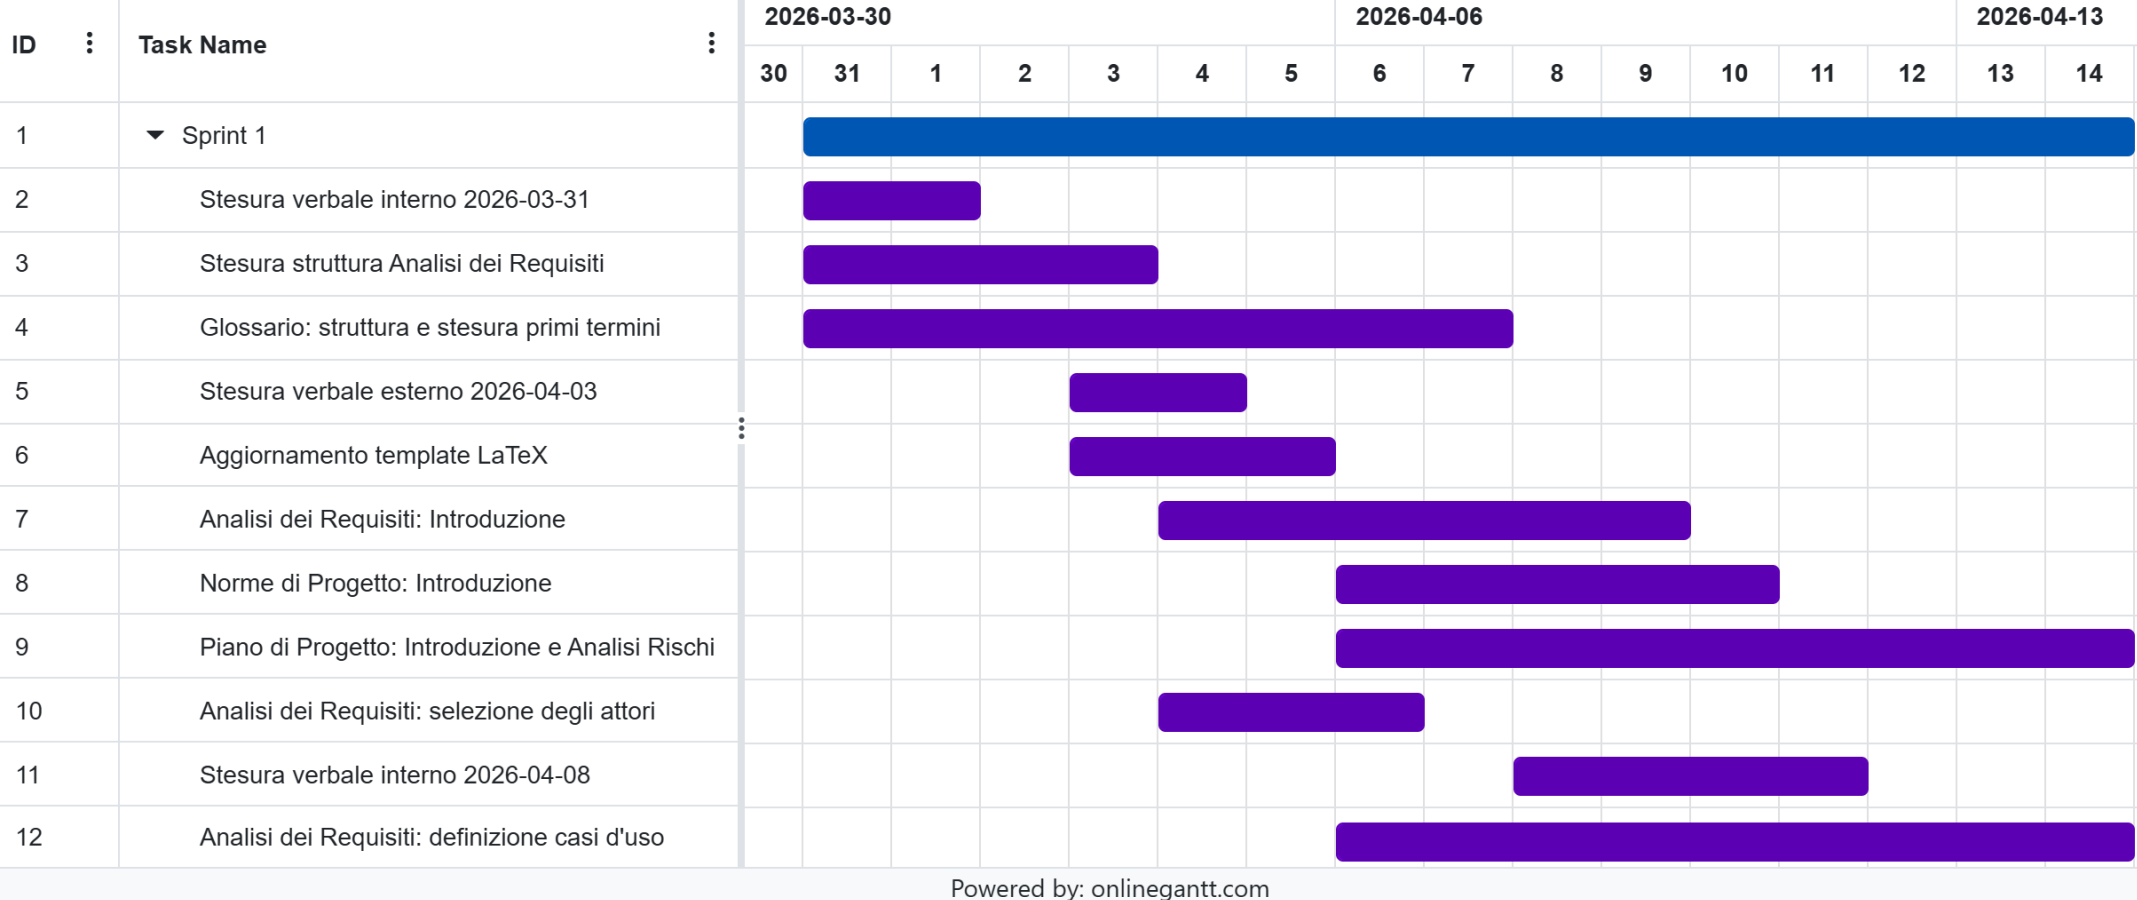
\includegraphics[width=\textwidth]{assets/gantt-sprint-1.png}
    \caption{Diagramma di Gantt dello Sprint 1}
    \label{fig:gantt-sprint1}
\end{figure}

\subsection{Sprint \#2: da 2026-04-14 a 2026-04-27}

\subsubsection{Obiettivi}
Durante il secondo sprint, il team prevede di consolidare e aggiornare la documentazione prodotta nello sprint\textsubscript{G} precedente, con particolare attenzione all'avanzamento dell'\textit{Analisi dei Requisiti}. L'obiettivo principale è passare dalla fase preliminare di studio e modellazione alla stesura più formale dei casi d'uso\textsubscript{G}, mantenendo allineati il \textit{Piano di Progetto}, le \textit{Norme di Progetto}, il \textit{Glossario} e l'\textit{Analisi dei Requisiti}.
Nello specifico, il team si impegnerà a:
\begin{itemize}
    \item proseguire la stesura del documento \textit{Analisi dei Requisiti}, avviando la descrizione formale dei casi d'uso\textsubscript{G} precedentemente studiati e modellati;

    \item completare la prima versione delle \textit{Norme di Progetto}, così da fornire al gruppo una base normativa condivisa per la gestione del lavoro, della documentazione e degli strumenti utilizzati;

    \item completare, all'interno del \textit{Piano di Progetto}, la sezione relativa all'analisi e alla gestione dei rischi e redigere il consuntivo e la retrospettiva dello Sprint\textsubscript{G} \#1, analizzando gli scostamenti rispetto al preventivo e individuando eventuali azioni correttive;

    \item aggiornare il \textit{Glossario} con i termini tecnici emersi durante la stesura della documentazione e durante le attività di analisi;

    \item avviare un'attività di brainstorming per il design preliminare UX/UI\textsubscript{G}, in vista della preparazione del mock-up\textsubscript{G} previsto per lo Sprint\textsubscript{G} \#3;

    \item redigere i verbali interni ed esterni relativi agli incontri svolti durante lo sprint\textsubscript{G}.
\end{itemize}

\begin{figure}[H]
    \centering
    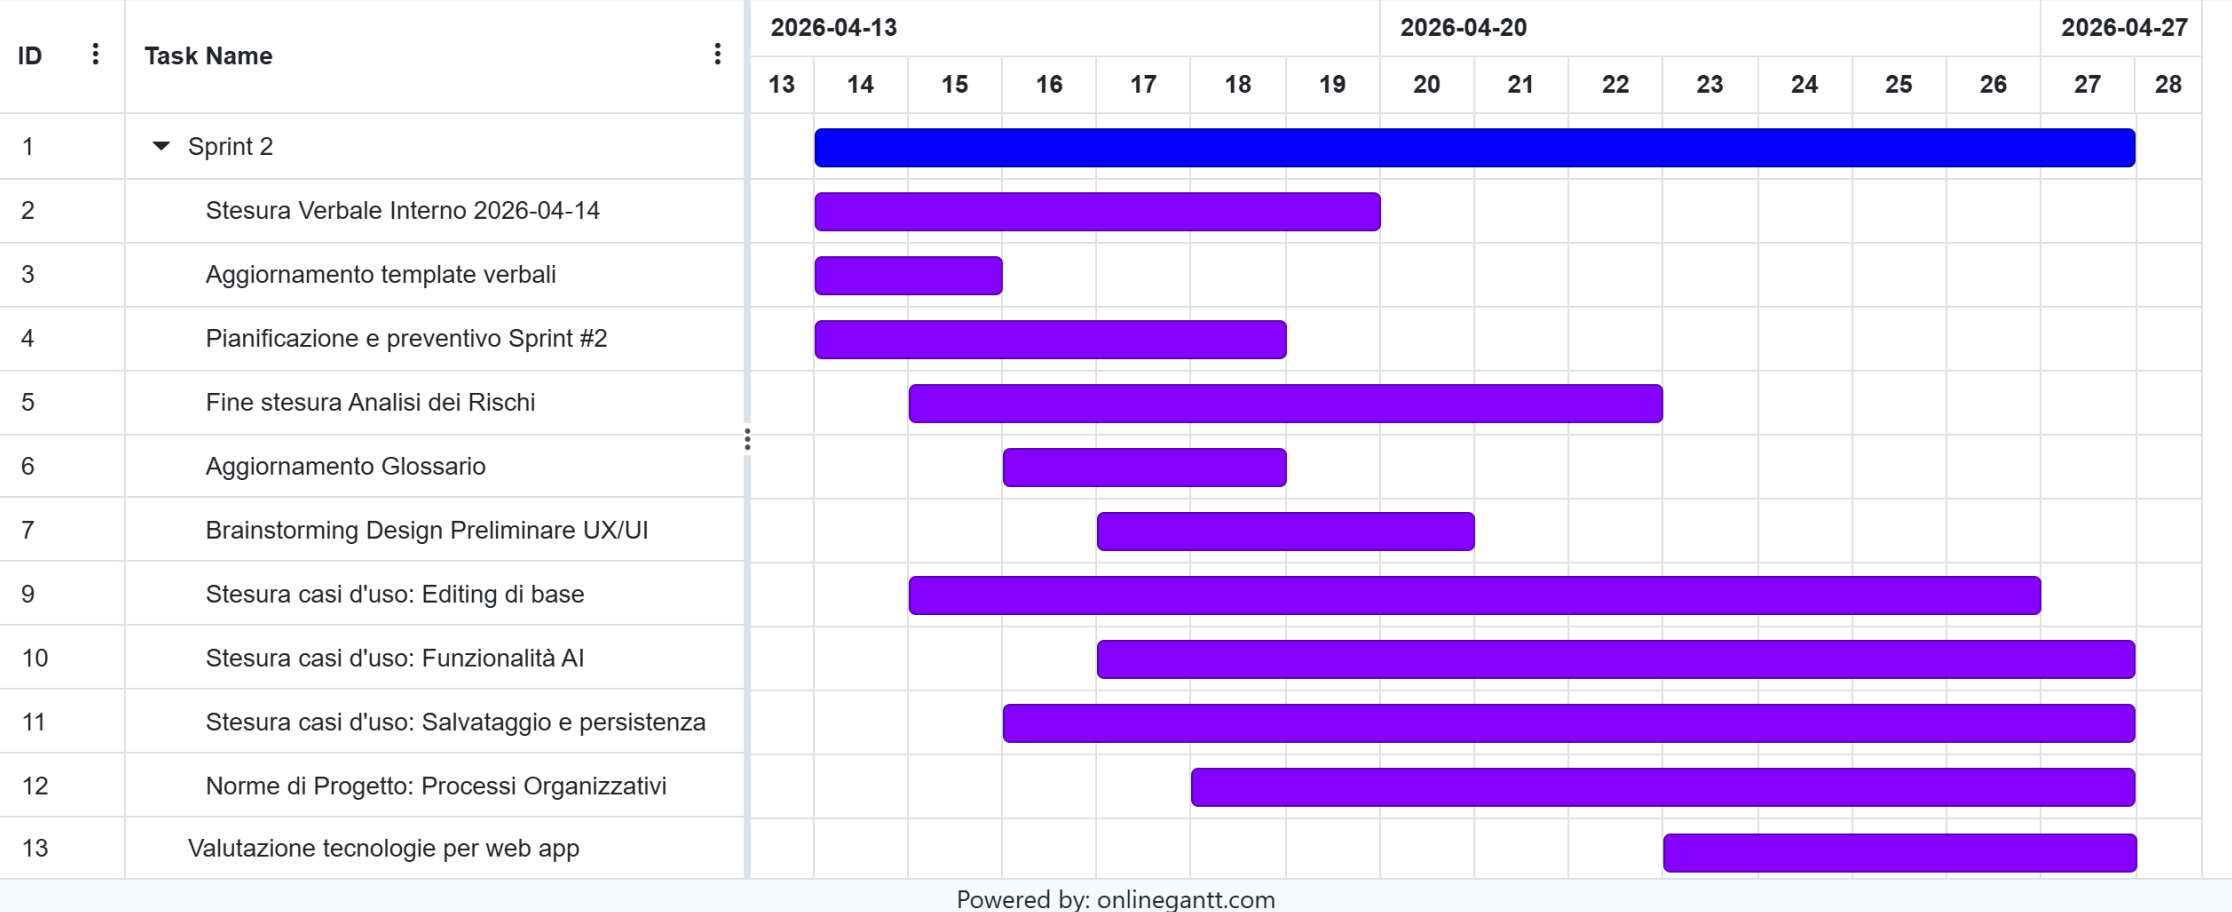
\includegraphics[width=\textwidth]{assets/gantt-sprint-2.png}
    \caption{Diagramma di Gantt dello Sprint 2}
    \label{fig:gantt-sprint2}
\end{figure}

\subsection{Sprint \#3: da 2026-04-28 a 2026-05-11}
\subsubsection{Obiettivi}
Durante il terzo sprint\textsubscript{G}, il team prevede di concentrare le attività sul completamento dell'\textit{Analisi dei Requisiti} e sull'avvio delle prime attività progettuali legate al prodotto software. 
In questo sprint\textsubscript{G} viene inoltre introdotto il ruolo di Progettista, principalmente per la realizzazione del mock-up\textsubscript{G} dell'interfaccia utente e per le prime attività di raccordo tra requisiti, esperienza utente e futura implementazione del prodotto.
Nello specifico, il team si impegnerà a:
\begin{itemize}
    \item completare l'\textit{Analisi dei Requisiti}, realizzando i diagrammi UML\textsubscript{G} relativi ai casi d'uso\textsubscript{G};

    \item organizzare un incontro con la Proponente\textsubscript{G} per discutere i casi d'uso individuati, chiarire eventuali ambiguità e ottenere un riscontro prima di procedere con le fasi successive del progetto;

    \item avviare la realizzazione del mock-up\textsubscript{G} dell'interfaccia utente, definendo una prima rappresentazione grafica delle principali schermate e dei flussi di interazione dell'applicazione;

    \item svolgere uno studio iniziale delle tecnologie da adottare nello sviluppo del prodotto software, valutando quali strumenti risultino più adeguati per la realizzazione della web app\textsubscript{G};

    \item proseguire l'aggiornamento dei documenti di progetto, in particolare \textit{Piano di Progetto}, \textit{Norme di Progetto}, \textit{Glossario} e \textit{Analisi dei Requisiti};

    \item sviluppare uno script\textsubscript{G} per automatizzare la gestione dei termini del \textit{Glossario}, riducendo il lavoro manuale necessario per inserire nei documenti il riferimento ai termini glossarizzati;
    \item redigere i verbali interni ed esterni relativi agli incontri svolti durante lo sprint\textsubscript{G}.
\end{itemize}

\begin{figure}[H]
    \centering
    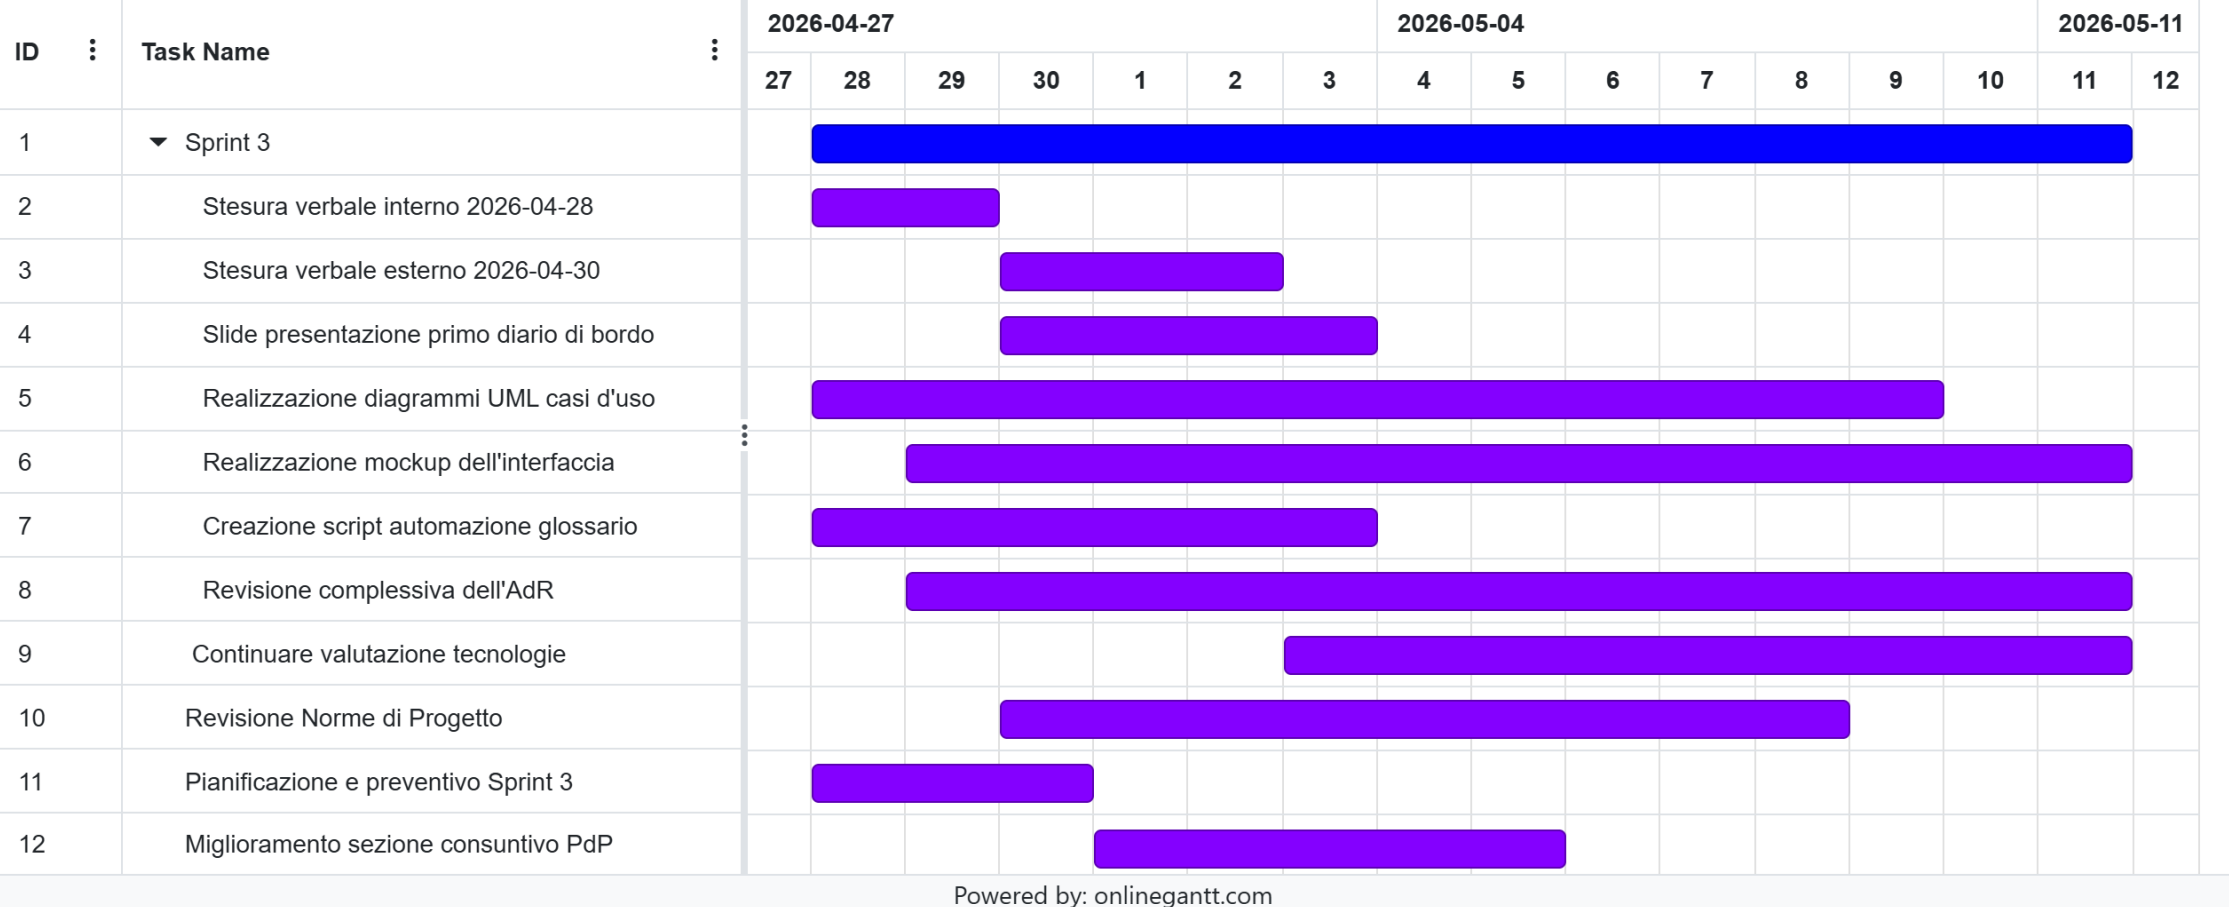
\includegraphics[width=\textwidth]{assets/gantt-sprint-3.png}
    \caption{Diagramma di Gantt dello Sprint 3}
    \label{fig:gantt-sprint3}
\end{figure}


\subsection{Sprint \#4: da 2026-05-12 a 2026-05-25}

\subsubsection{Obiettivi}

Durante il quarto sprint\textsubscript{G}, il team prevede di concentrarsi principalmente sulla realizzazione del \textit{Proof of Concept} e sulla definizione dell'architettura logica necessaria a supportare le funzionalità richieste dal capitolato C6 - \textit{Second Brain}.
\begin{itemize}
    \item consolidare definitivamente il documento di Analisi dei Requisiti in ogni sua sezione;
    \item prendere le decisioni formali e definitive sullo stack tecnologico e sui framework da adottare per lo sviluppo del \textit{Proof of Concept} e del prodotto software finale;
    \item avviare uno studio iniziale per definire l'architettura logica del PoC e comprendere i requisiti minimi necessari alla sua progettazione;
    \item introdurre formalmente il ruolo di Programmatore, che lavorerà in sinergia con il Progettista per l'avvio delle attività tecniche legate al \textit{Proof of Concept};
    \item iniziare lo sviluppo e la codifica effettiva del PoC verso la conclusione dello sprint;
    \item avviare un percorso di formazione per allineare tutti i componenti del gruppo sulle tecnologie scelte;
    \item proseguire con l'aggiornamento e la stesura della documentazione di supporto.
\end{itemize}

\begin{figure}[H]
    \centering
    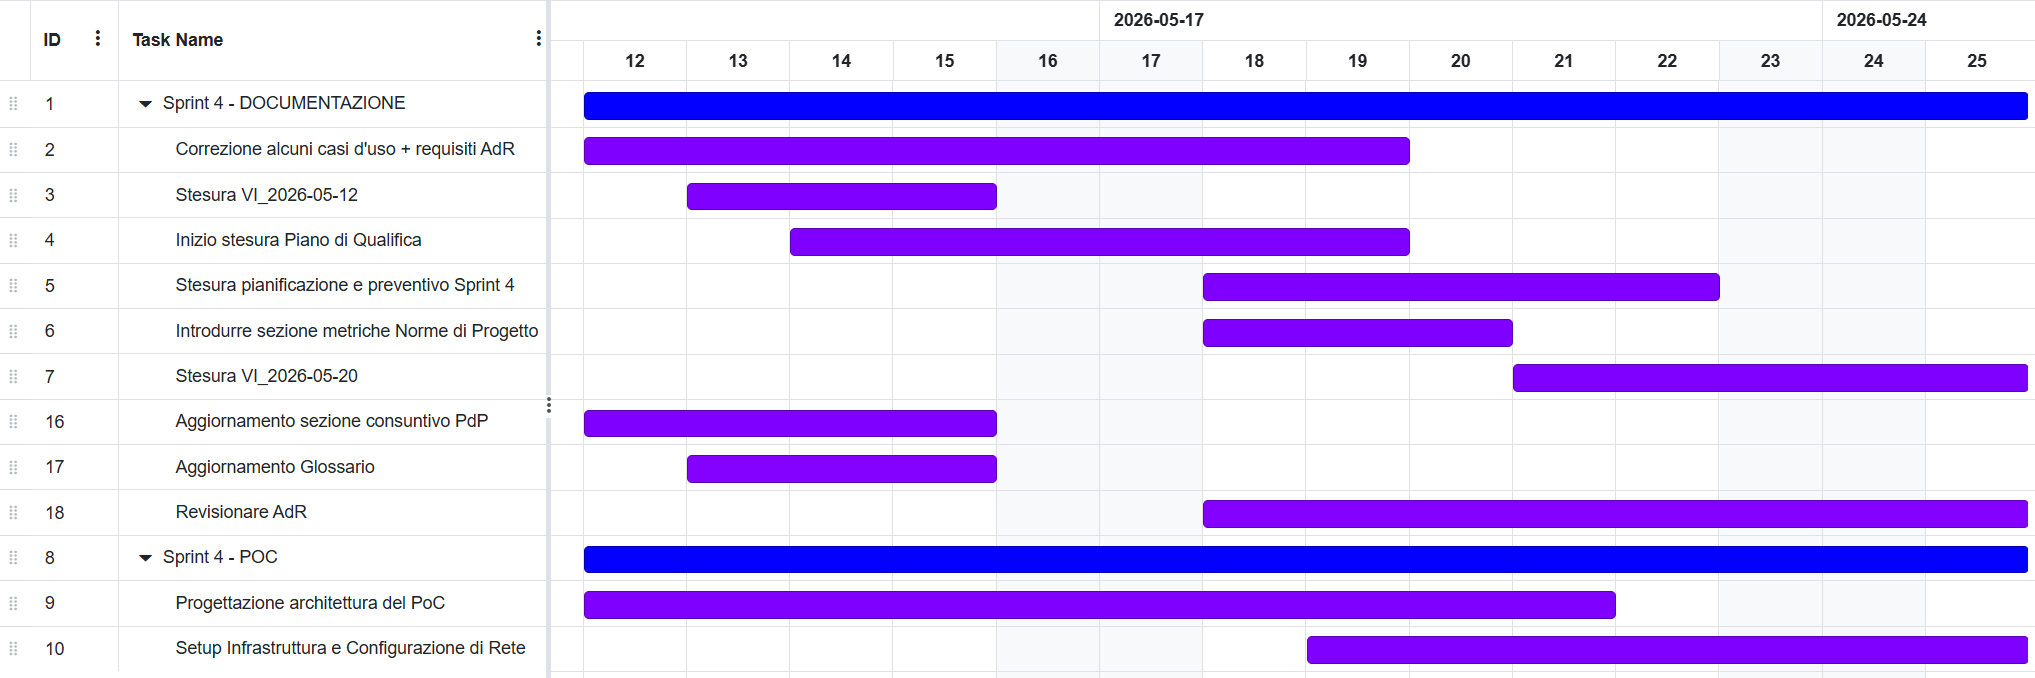
\includegraphics[width=\textwidth]{assets/gantt-sprint-4.png}
    \caption{Diagramma di Gantt dello Sprint 4}
    \label{fig:gantt-sprint4}
\end{figure}

\subsection{Sprint \#5: da 2026-05-26 a 2026-06-08}

\subsubsection{Obiettivi}
Gli obiettivi dello Sprint\textsubscript{G} \#5 sono stati definiti a partire dalle evidenze emerse nella retrospettiva precedente e in coerenza con l'avanzamento complessivo del progetto. L'attività centrale dell'iterazione è il completamento del \textit{Proof of Concept}, affiancata dalla stesura del \textit{Piano di Qualifica} e dalla revisione di correttezza dei documenti già prodotti.

Per concentrare l'impegno sullo sviluppo, il team ha previsto l'impiego di tre Programmatori\textsubscript{G}, dedicati in parallelo al front-end e al back-end del PoC, e di un Verificatore\textsubscript{G} incaricato di controllare in modo continuativo quanto via via implementato.

Nello specifico, il team si impegnerà a:
\begin{itemize}
    \item completare lo sviluppo del \textit{Proof of Concept}, portando a termine entro la finestra dello sprint\textsubscript{G} l'implementazione del front-end e del back-end e la verifica delle componenti realizzate;

    \item proseguire la stesura del \textit{Piano di Qualifica}, con particolare attenzione alla sezione dedicata alle metriche di prodotto, che saranno popolate a partire dai test\textsubscript{G} effettivamente eseguiti sul PoC: la disponibilità di codice funzionante consentirà di passare da definizioni astratte a misurazioni concrete;

    \item revisionare la correttezza dei documenti già prodotti, correggendo eventuali refusi, aggiornando i riferimenti incrociati e allineando i contenuti allo stato corrente del progetto, con particolare riguardo alle \textit{Norme di Progetto};

    \item aggiornare il \textit{Piano di Progetto} per riflettere i consuntivi dello Sprint\textsubscript{G} \#4 e la pianificazione rivista per gli sprint\textsubscript{G} successivi;

    \item avanzare il \textit{Glossario} con i nuovi termini emersi durante lo sviluppo e la progettazione, integrandolo nel sito pubblico del gruppo affinché risulti direttamente consultabile online;

    \item migliorare la veste grafica e l'organizzazione del sito pubblico del progetto;

    \item proseguire l'attività di studio e approfondimento delle tecnologie adottate per lo sviluppo del PoC;

    \item redigere i verbali interni ed esterni relativi agli incontri svolti durante lo sprint\textsubscript{G}.
\end{itemize}

\begin{figure}[H]
    \centering
    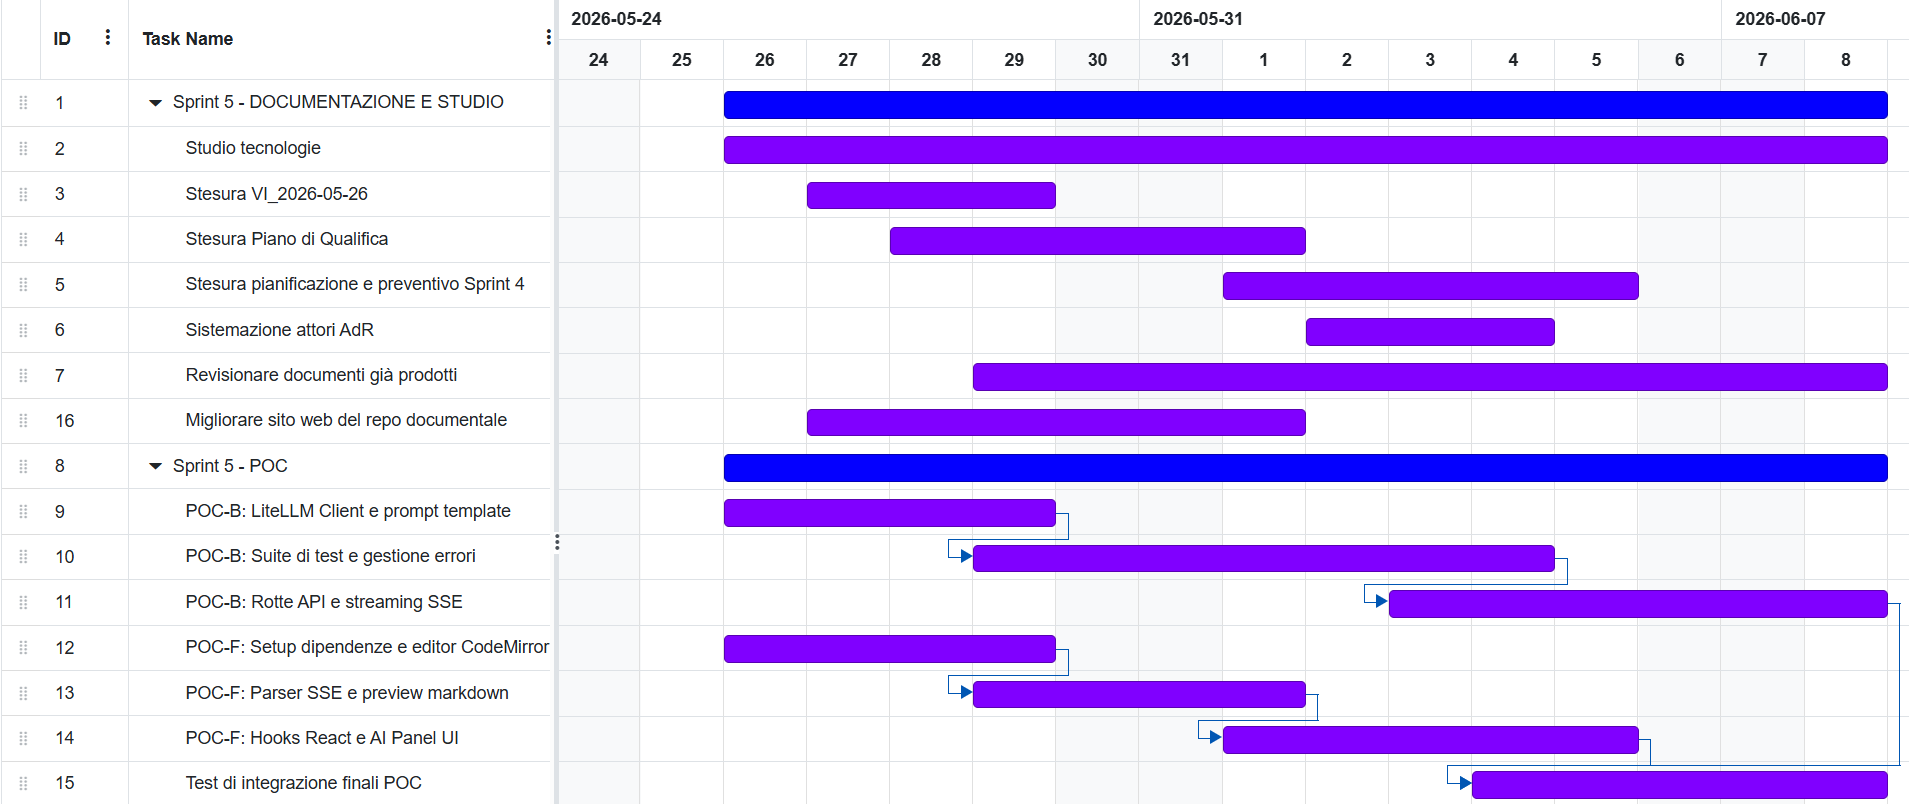
\includegraphics[width=\textwidth]{assets/gantt-sprint-5.png}
    \caption{Diagramma di Gantt dello Sprint 5}
    \label{fig:gantt-sprint5}
\end{figure}

\subsection{Sprint \#6: da 2026-06-09 a 2026-06-22}

\subsubsection{Obiettivi}
Lo Sprint\textsubscript{G} \#6 è dedicato principalmente ad attività di programmazione e di verifica\textsubscript{G}, in vista della presentazione della RTB\textsubscript{G}. L'obiettivo centrale è il completamento del \textit{Proof of Concept} e il controllo accurato di tutta la documentazione prodotta finora.

Nello specifico, il team si impegnerà a:
\begin{itemize}
    \item completare lo sviluppo del \textit{Proof of Concept};
    \item verificare accuratamente tutti i documenti in vista della presentazione della RTB\textsubscript{G}, con particolare attenzione all'\textit{Analisi dei Requisiti}, alle \textit{Norme di Progetto} e al \textit{Piano di Progetto};
    \item completare il \textit{Piano di Qualifica} e sottoporlo a un'accurata verifica\textsubscript{G};
    \item organizzare un incontro con la Proponente\textsubscript{G} per mostrare il \textit{Proof of Concept} e raccoglierne il riscontro;
    \item preparare le diapositive per la presentazione RTB\textsubscript{G} delle tecnologie;
    \item redigere la lettera di presentazione destinata al prof. Cardin;
    \item richiedere al prof. Cardin il colloquio per la presentazione delle tecnologie della RTB\textsubscript{G};
    \item redigere i verbali interni ed esterni relativi agli incontri svolti durante lo sprint\textsubscript{G}.
\end{itemize}

\begin{figure}[H]
    \centering
    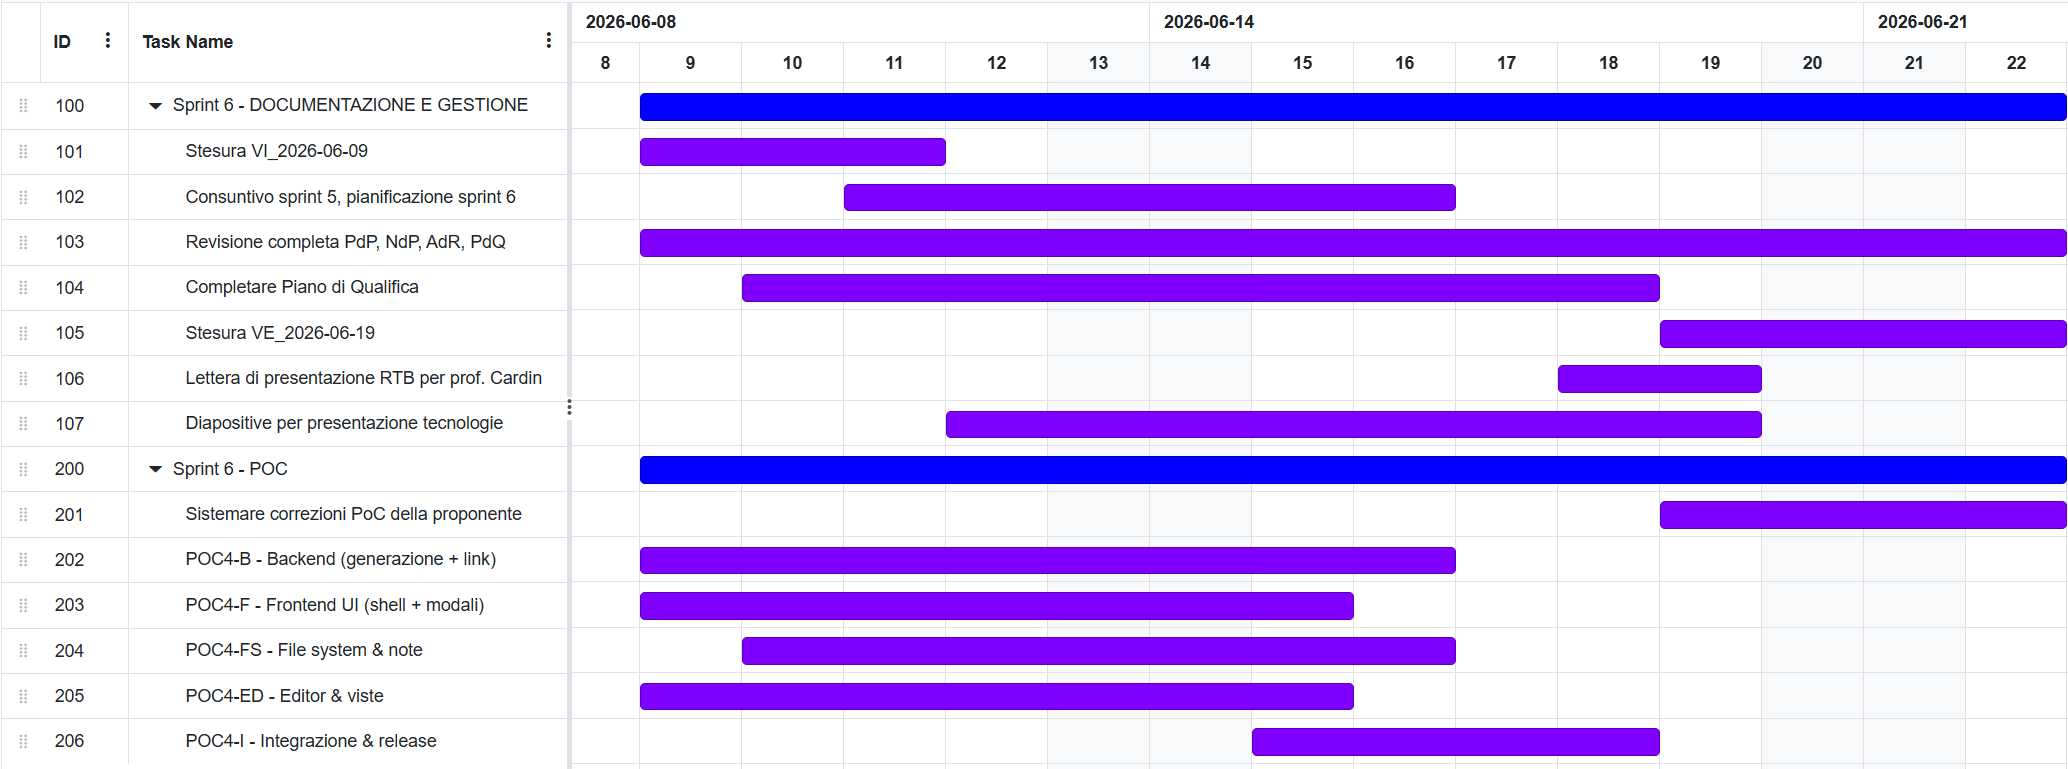
\includegraphics[width=\textwidth]{assets/gantt-sprint-6.png}
    \caption{Diagramma di Gantt dello Sprint 6}
    \label{fig:gantt-sprint6}
\end{figure}

\subsection{Sprint \#7: da 2026-06-23 a 2026-07-06}

\subsubsection{Obiettivi}
Lo Sprint\textsubscript{G} \#7 comprende la consegna della RTB\textsubscript{G}, avvenuta il 25 giugno 2026 con circa cinque giorni di ritardo rispetto a quanto pianificato per lo Sprint\textsubscript{G} \#6, ed è dedicato alla formalizzazione della candidatura per la presentazione delle tecnologie, all'attesa del riscontro da parte del prof. Cardin e al consolidamento della documentazione, oltre a un'intensa attività di palestra in preparazione della fase successiva di Progettazione e Codifica.

Nello specifico, il team si impegnerà a:
\begin{itemize}
    \item inoltrare al prof. Cardin la candidatura per il colloquio di presentazione delle tecnologie della RTB\textsubscript{G}, svolgere la relativa presentazione e attenderne il riscontro;
    \item redigere la lettera di presentazione della RTB\textsubscript{G} destinata al prof. Vardanega;
    \item aggiornare i documenti soggetti a modifica, in particolare il \textit{Piano di Progetto} (con l'aggiunta del consuntivo dello Sprint\textsubscript{G} \#6 e della pianificazione e del preventivo dello Sprint\textsubscript{G} \#7) e il \textit{Piano di Qualifica} (con l'aggiunta degli Sprint\textsubscript{G} \#6 e \#7);
    \item approvare tutti i documenti per l'ingresso nella baseline\textsubscript{G} della RTB\textsubscript{G};
    \item avviare la progettazione dell'MVP\textsubscript{G}, limitatamente alla progettazione e senza attività di codifica;
    \item analizzare i documenti da produrre nella fase di Product Baseline\textsubscript{G}, in particolare il \textit{Manuale Utente} e la \textit{Specifica Tecnica};
    \item dedicare ore di palestra all'approfondimento delle tecnologie e alla preparazione delle attività iniziali della Product Baseline\textsubscript{G}.
\end{itemize}

Il gruppo attribuisce particolare importanza alle ore di palestra: prima di avviare concretamente le attività di sviluppo è infatti fondamentale comprendere \textit{come} realizzarle. Si tratta di ore che non vengono rendicontate come effettivamente produttive, ma che risultano essenziali per costruire una base solida su cui impostare il lavoro della fase successiva.

\begin{figure}[H]
    \centering
    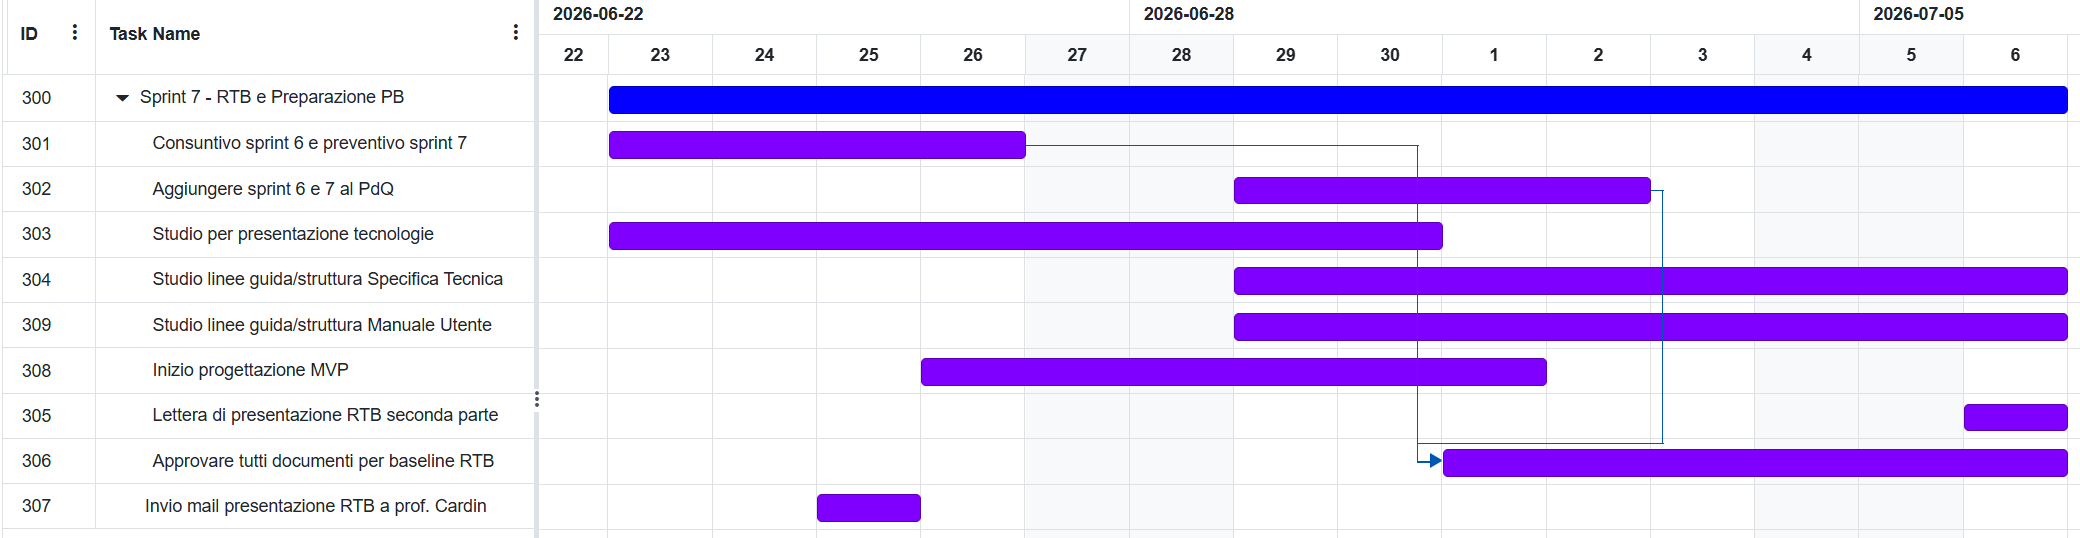
\includegraphics[width=\textwidth]{assets/gantt-sprint-7.png}
    \caption{Diagramma di Gantt dello Sprint 7}
    \label{fig:gantt-sprint7}
\end{figure}

\section{Preventivo}
Il preventivo viene elaborato considerando il costo orario associato a ciascun ruolo, il budget complessivo previsto e le attività pianificate per il periodo di riferimento. Per ogni sprint\textsubscript{G} vengono quindi riportati:

\begin{itemize}
    \item un preventivo delle ore previste, organizzato in forma tabellare;
    \item un preventivo dei costi stimati, anch'esso presentato in forma tabellare;
    \item un areogramma che rappresenta la distribuzione delle ore tra i diversi ruoli di progetto.
\end{itemize}

Il carico di lavoro complessivo previsto per ciascun componente del gruppo è pari a 92 ore, distribuite tra i diversi ruoli di progetto, per un totale di 644 ore produttive. La ripartizione delle mansioni viene gestita tramite un meccanismo di rotazione, con l'obiettivo di garantire a ogni membro del team la possibilità di ricoprire ruoli differenti e acquisire una visione più completa del processo di sviluppo.

Per rendere le tabelle più leggibili e compatte, i ruoli di progetto vengono indicati mediante le seguenti abbreviazioni\textsubscript{G}:

\begin{itemize}
    \item \textbf{Re}: Responsabile di progetto;
    \item \textbf{Am}: Amministratore;
    \item \textbf{An}: Analista;
    \item \textbf{Pt}: Progettista;
    \item \textbf{Pr}: Programmatore;
    \item \textbf{Ve}: Verificatore.
\end{itemize}

\subsection{Sprint \#1: da 2026-03-31 a 2026-04-13}
Di seguito è riportata la distribuzione delle ore per ciascun membro del team,
accumulate in totali per persona e per ruolo:

\begin{table}[H]
    \centering
    \renewcommand{\arraystretch}{1.4}
    \begin{tabular}{|l|c|c|c|c|c|c|c|}
        \hline
        \rowcolor{bluBitless!15}
        \textbf{Membro} & \textbf{Re} & \textbf{Am} & \textbf{An} & \textbf{Pt} & \textbf{Pr} & \textbf{Ve} & \textbf{Totale per persona} \\
        \hline
        L. Battistella & - & - & 6 & - & - & - & 6 \\ \hline
        E. De Piccoli & - & 5 & - & - & - & - & 5 \\ \hline
        D. Facco & - & - & 6 & - & - & - & 6 \\ \hline
        A. Marini & - & - & 6 & - & - & - & 6 \\ \hline
        A. Menegaldo & - & - & - & - & - & 8 & 8 \\ \hline
        S. Vendramin & 4 & - & - & - & - & - & 4 \\ \hline
        S. Zecchinato & - & - & 6 & - & - & - & 6 \\ \hline
        \rowcolor{bluBitless!8}
        \textbf{Totale per ruolo} & \textbf{4} & \textbf{5} & \textbf{24} & \textbf{-} & \textbf{-} & \textbf{8} & \textbf{41} \\
        \hline
    \end{tabular}
    \caption{\textit{Preventivo orario Sprint \#1}}
\end{table}

\begin{figure}[H]
\centering

\begin{tikzpicture}[scale=0.85]

% Colori pastello
\definecolor{colResp}{HTML}{BFE8DD}
\definecolor{colAmm}{HTML}{FFD0B5}
\definecolor{colAn}{HTML}{E4C9F5}
\definecolor{colVe}{HTML}{CDEBFF}
\definecolor{lineGray}{HTML}{8A8A8A}

% Raggio dell'areogramma
\def\r{3.2}

% Titolo
\node[font=\Large\bfseries] at (0,4.25) {Distribuzione ore per ruolo};

% Settori
% Totale = 41
% Re = 4 -> 9,8%
% Am = 5 -> 12,2%
% An = 24 -> 58,5%
% Ve = 8 -> 19,5%

\path[fill=colResp, draw=white, line width=1.5pt]
(0,0) -- (90:\r) arc[start angle=90,end angle=54.9,radius=\r] -- cycle;

\path[fill=colAmm, draw=white, line width=1.5pt]
(0,0) -- (54.9:\r) arc[start angle=54.9,end angle=11.0,radius=\r] -- cycle;

\path[fill=colAn, draw=white, line width=1.5pt]
(0,0) -- (11.0:\r) arc[start angle=11.0,end angle=-199.7,radius=\r] -- cycle;

\path[fill=colVe, draw=white, line width=1.5pt]
(0,0) -- (-199.7:\r) arc[start angle=-199.7,end angle=-270,radius=\r] -- cycle;

% Percentuali interne più piccole
\node[font=\normalsize\bfseries] at (70:1.75) {9,8\%};
\node[font=\normalsize\bfseries] at (31:1.85) {12,2\%};
\node[font=\normalsize\bfseries] at (-98:1.55) {58,5\%};
\node[font=\normalsize\bfseries] at (131:1.85) {19,5\%};

% Linee ed etichette esterne - Responsabile
\fill[lineGray] (1.25,2.75) circle (1.7pt);
\draw[lineGray, line width=0.7pt] (1.25,2.75) -- (3.65,2.75) -- (5.5,2.75);
\node[anchor=south east, font=\normalsize\bfseries] at (5.5,2.82) {Responsabile};
\node[anchor=north east, font=\small\bfseries, text=lineGray] at (5.5,2.60) {4 ore};

% Linee ed etichette esterne - Amministratore
\fill[lineGray] (2.85,1.05) circle (1.7pt);
\draw[lineGray, line width=0.7pt] (2.85,1.05) -- (4.0,1.05) -- (5.55,1.05);
\node[anchor=south east, font=\normalsize\bfseries] at (5.55,1.12) {Amministratore};
\node[anchor=north east, font=\small\bfseries, text=lineGray] at (5.55,0.90) {5 ore};

% Linee ed etichette esterne - Analista
\fill[lineGray] (-1.35,-2.65) circle (1.7pt);
\draw[lineGray, line width=0.7pt] (-1.35,-2.65) -- (-3.65,-2.65) -- (-5.45,-2.65);
\node[anchor=south west, font=\normalsize\bfseries] at (-5.45,-2.58) {Analista};
\node[anchor=north west, font=\small\bfseries, text=lineGray] at (-5.45,-2.80) {24 ore};

% Linee ed etichette esterne - Verificatore
\fill[lineGray] (-2.15,2.35) circle (1.7pt);
\draw[lineGray, line width=0.7pt] (-2.15,2.35) -- (-3.9,2.35) -- (-5.45,2.35);
\node[anchor=south west, font=\normalsize\bfseries] at (-5.45,2.42) {Verificatore};
\node[anchor=north west, font=\small\bfseries, text=lineGray] at (-5.45,2.20) {8 ore};

\end{tikzpicture}

\caption{Areogramma del preventivo orario nello Sprint \#1}
\label{fig:preventivo-sprint1}
\end{figure}

Di seguito è riportato il preventivo economico del primo sprint\textsubscript{G}:

\begin{table}[H]
    \centering
    \renewcommand{\arraystretch}{1.4}
    \begin{tabular}{|l|c|c|}
        \hline
        \rowcolor{bluBitless!15}
        \textbf{Ruolo} & \textbf{Ore per ruolo} & \textbf{Costo (in €)} \\
        \hline
        Responsabile di progetto & 4 & 120,00 \\ \hline
        Amministratore & 5 & 100,00 \\ \hline
        Analista & 24 & 600,00 \\ \hline
        Progettista & 0 & 0,00 \\ \hline
        Programmatore & 0 & 0,00 \\ \hline
        Verificatore & 8 & 120,00 \\ \hline
        \rowcolor{bluBitless!8}
        \textbf{Totale} & \textbf{41} & \textbf{940,00} \\ \hline
    \end{tabular}
    \caption{\textit{Preventivo economico dello Sprint \#1}}
\end{table}

\subsection{Sprint \#2: da 2026-04-14 a 2026-04-27}
Di seguito è riportata la distribuzione delle ore per ciascun membro del team,
accumulate in totali per persona e per ruolo:
\begin{table}[H]
    \centering
    \renewcommand{\arraystretch}{1.4}
    \begin{tabular}{|l|c|c|c|c|c|c|c|}
        \hline
        \rowcolor{bluBitless!15}
        \textbf{Membro} & \textbf{Re} & \textbf{Am} & \textbf{An} & \textbf{Pt} & \textbf{Pr} & \textbf{Ve} & \textbf{Totale per persona} \\
        \hline
        L. Battistella & 7 & - & - & - & - & - & 7 \\ \hline
        E. De Piccoli & - & - & - & - & - & 6 & 6 \\ \hline
        D. Facco & - & - & - & - & - & 6 & 6 \\ \hline
        A. Marini & - & 7 & - & - & - & - & 7 \\ \hline
        A. Menegaldo & - & - & 6 & - & - & - & 6 \\ \hline
        S. Vendramin & - & - & 6 & - & - & - & 6 \\ \hline
        S. Zecchinato & - & - & 6 & - & - & - & 6 \\ \hline
        \rowcolor{bluBitless!8}
        \textbf{Totale per ruolo} & \textbf{7} & \textbf{7} & \textbf{18} & \textbf{-} & \textbf{-} & \textbf{12} & \textbf{44} \\
        \hline
    \end{tabular}
    \caption{\textit{Preventivo orario Sprint \#2}}
\end{table}

\begin{figure}[H]
\centering

\begin{tikzpicture}[scale=0.85]

% Colori pastello
\definecolor{colResp}{HTML}{BFE8DD}
\definecolor{colAmm}{HTML}{FFD0B5}
\definecolor{colAn}{HTML}{E4C9F5}
\definecolor{colVe}{HTML}{CDEBFF}
\definecolor{lineGray}{HTML}{8A8A8A}

% Raggio dell'areogramma
\def\r{3.2}

% Titolo
\node[font=\Large\bfseries] at (0,4.25) {Distribuzione ore per ruolo};

% Totale = 44
% Re = 7 -> 15,9%
% Am = 7 -> 15,9%
% An = 18 -> 40,9%
% Ve = 12 -> 27,3%

% Settori
\path[fill=colResp, draw=white, line width=1.5pt]
(0,0) -- (90:\r) arc[start angle=90,end angle=32.7,radius=\r] -- cycle;

\path[fill=colAmm, draw=white, line width=1.5pt]
(0,0) -- (32.7:\r) arc[start angle=32.7,end angle=-24.5,radius=\r] -- cycle;

\path[fill=colAn, draw=white, line width=1.5pt]
(0,0) -- (-24.5:\r) arc[start angle=-24.5,end angle=-171.8,radius=\r] -- cycle;

\path[fill=colVe, draw=white, line width=1.5pt]
(0,0) -- (-171.8:\r) arc[start angle=-171.8,end angle=-270,radius=\r] -- cycle;

% Percentuali interne
\node[font=\normalsize\bfseries] at (65:1.75) {15,9\%};
\node[font=\normalsize\bfseries] at (10:1.85) {15,9\%};
\node[font=\normalsize\bfseries] at (-95:1.55) {40,9\%};
\node[font=\normalsize\bfseries] at (140:1.85) {27,3\%};

% Linee ed etichette esterne - Responsabile
\fill[lineGray] (1.60,2.50) circle (1.7pt);
\draw[lineGray, line width=0.7pt] (1.60,2.50) -- (3.65,2.50) -- (5.5,2.50);
\node[anchor=south east, font=\normalsize\bfseries] at (5.5,2.57) {Responsabile};
\node[anchor=north east, font=\small\bfseries, text=lineGray] at (5.5,2.35) {7 ore};

% Linee ed etichette esterne - Amministratore
\fill[lineGray] (3.00,0.35) circle (1.7pt);
\draw[lineGray, line width=0.7pt] (3.00,0.35) -- (4.0,0.35) -- (5.55,0.35);
\node[anchor=south east, font=\normalsize\bfseries] at (5.55,0.42) {Amministratore};
\node[anchor=north east, font=\small\bfseries, text=lineGray] at (5.55,0.20) {7 ore};

% Linee ed etichette esterne - Analista
\fill[lineGray] (-0.70,-3.00) circle (1.7pt);
\draw[lineGray, line width=0.7pt] (-0.70,-3.00) -- (-3.65,-3.00) -- (-5.45,-3.00);
\node[anchor=south west, font=\normalsize\bfseries] at (-5.45,-2.93) {Analista};
\node[anchor=north west, font=\small\bfseries, text=lineGray] at (-5.45,-3.15) {18 ore};

% Linee ed etichette esterne - Verificatore
\fill[lineGray] (-2.20,2.30) circle (1.7pt);
\draw[lineGray, line width=0.7pt] (-2.20,2.30) -- (-3.9,2.30) -- (-5.45,2.30);
\node[anchor=south west, font=\normalsize\bfseries] at (-5.45,2.37) {Verificatore};
\node[anchor=north west, font=\small\bfseries, text=lineGray] at (-5.45,2.15) {12 ore};

\end{tikzpicture}

\caption{Areogramma della distribuzione delle ore per ruolo nello Sprint \#2}
\label{fig:preventivo-sprint2}
\end{figure}

Di seguito è riportato il preventivo economico del secondo sprint\textsubscript{G}:

\begin{table}[H]
    \centering
    \renewcommand{\arraystretch}{1.4}
    \begin{tabular}{|l|c|c|}
        \hline
        \rowcolor{bluBitless!15}
        \textbf{Ruolo} & \textbf{Ore per ruolo} & \textbf{Costo (in €)} \\
        \hline
        Responsabile di progetto & 7 & 210,00 \\ \hline
        Amministratore & 7 & 140,00 \\ \hline
        Analista & 18 & 450,00 \\ \hline
        Progettista & 0 & 0,00 \\ \hline
        Programmatore & 0 & 0,00 \\ \hline
        Verificatore & 12 & 180,00 \\ \hline
        \rowcolor{bluBitless!8}
        \textbf{Totale} & \textbf{44} & \textbf{980,00} \\ \hline
    \end{tabular}
    \caption{\textit{Preventivo economico dello Sprint \#2}}
\end{table}


\subsection{Sprint \#3: da 2026-04-28 a 2026-05-11}
Di seguito è riportata la distribuzione delle ore per ciascun membro del team,
accumulate in totali per persona e per ruolo:

\begin{table}[H]
    \centering
    \renewcommand{\arraystretch}{1.4}
    \begin{tabular}{|l|c|c|c|c|c|c|c|}
        \hline
        \rowcolor{bluBitless!15}
        \textbf{Membro} & \textbf{Re} & \textbf{Am} & \textbf{An} & \textbf{Pt} & \textbf{Pr} & \textbf{Ve} & \textbf{Totale per persona} \\
        \hline
        L. Battistella & - & 7 & - & - & - & - & 7 \\ \hline
        E. De Piccoli & - & - & 7 & - & - & - & 7 \\ \hline
        D. Facco & - & - & - & 5 & - & - & 5 \\ \hline
        A. Marini & 4 & - & 3 & - & - & - & 7 \\ \hline
        A. Menegaldo & - & - & - & 5 & - & - & 5 \\ \hline
        S. Vendramin & - & - & - & - & - & 6 & 6 \\ \hline
        S. Zecchinato & - & - & - & - & - & 7 & 7 \\ \hline
        \rowcolor{bluBitless!8}
        \textbf{Totale per ruolo} & \textbf{4} & \textbf{7} & \textbf{10} & \textbf{10} & \textbf{-} & \textbf{13} & \textbf{44} \\
        \hline
    \end{tabular}
    \caption{\textit{Preventivo orario Sprint \#3}}
\end{table}

\begin{figure}[H]
\centering

\begin{tikzpicture}[scale=0.85]

% Colori pastello
\definecolor{colResp}{HTML}{BFD7EA}
\definecolor{colAmm}{HTML}{F7C8C8}
\definecolor{colAn}{HTML}{D8C4F2}
\definecolor{colPt}{HTML}{FFE5B4}
\definecolor{colVe}{HTML}{CDECCF}
\definecolor{lineGray}{HTML}{8A8A8A}

% Raggio dell'areogramma
\def\r{3.2}

% Titolo
\node[font=\Large\bfseries] at (0,4.25) {Distribuzione ore per ruolo};

% Totale = 44
% Re = 4  -> 9,1%
% Am = 7  -> 15,9%
% An = 10 -> 22,7%
% Pt = 10 -> 22,7%
% Ve = 13 -> 29,5%

% Settori
\path[fill=colResp, draw=white, line width=1.5pt]
(0,0) -- (90:\r) arc[start angle=90,end angle=57.3,radius=\r] -- cycle;

\path[fill=colAmm, draw=white, line width=1.5pt]
(0,0) -- (57.3:\r) arc[start angle=57.3,end angle=0.0,radius=\r] -- cycle;

\path[fill=colAn, draw=white, line width=1.5pt]
(0,0) -- (0.0:\r) arc[start angle=0.0,end angle=-81.8,radius=\r] -- cycle;

\path[fill=colPt, draw=white, line width=1.5pt]
(0,0) -- (-81.8:\r) arc[start angle=-81.8,end angle=-163.6,radius=\r] -- cycle;

\path[fill=colVe, draw=white, line width=1.5pt]
(0,0) -- (-163.6:\r) arc[start angle=-163.6,end angle=-270,radius=\r] -- cycle;

% Percentuali interne
\node[font=\small\bfseries] at (75:1.65) {9,1\%};
\node[font=\small\bfseries] at (36:1.75) {15,9\%};
\node[font=\small\bfseries] at (-25:1.75) {22,7\%};
\node[font=\small\bfseries] at (-118:1.75) {22,7\%};
\node[font=\small\bfseries] at (136:1.75) {29,5\%};

% Responsabile
\fill[lineGray] (0.95,2.90) circle (1.7pt);
\draw[lineGray, line width=0.7pt] (0.95,2.90) -- (3.65,2.90) -- (5.5,2.90);
\node[anchor=south east, font=\normalsize\bfseries] at (5.5,2.97) {Responsabile};
\node[anchor=north east, font=\small\bfseries, text=lineGray] at (5.5,2.75) {4 ore};

% Amministratore
\fill[lineGray] (2.75,1.25) circle (1.7pt);
\draw[lineGray, line width=0.7pt] (2.75,1.25) -- (4.0,1.25) -- (5.55,1.25);
\node[anchor=south east, font=\normalsize\bfseries] at (5.55,1.32) {Amministratore};
\node[anchor=north east, font=\small\bfseries, text=lineGray] at (5.55,1.10) {7 ore};

% Analista
\fill[lineGray] (2.65,-1.25) circle (1.7pt);
\draw[lineGray, line width=0.7pt] (2.65,-1.25) -- (4.0,-1.25) -- (5.55,-1.25);
\node[anchor=south east, font=\normalsize\bfseries] at (5.55,-1.18) {Analista};
\node[anchor=north east, font=\small\bfseries, text=lineGray] at (5.55,-1.40) {10 ore};

% Progettista
\fill[lineGray] (-1.85,-2.45) circle (1.7pt);
\draw[lineGray, line width=0.7pt] (-1.85,-2.45) -- (-3.75,-2.45) -- (-5.45,-2.45);
\node[anchor=south west, font=\normalsize\bfseries] at (-5.45,-2.38) {Progettista};
\node[anchor=north west, font=\small\bfseries, text=lineGray] at (-5.45,-2.60) {10 ore};

% Verificatore
\fill[lineGray] (-2.30,2.15) circle (1.7pt);
\draw[lineGray, line width=0.7pt] (-2.30,2.15) -- (-3.9,2.15) -- (-5.45,2.15);
\node[anchor=south west, font=\normalsize\bfseries] at (-5.45,2.22) {Verificatore};
\node[anchor=north west, font=\small\bfseries, text=lineGray] at (-5.45,2.00) {13 ore};

\end{tikzpicture}

\caption{Areogramma del preventivo orario nello Sprint \#3}
\label{fig:preventivo-sprint3}
\end{figure}

Di seguito è riportato il preventivo economico del terzo sprint\textsubscript{G}:

\begin{table}[H]
    \centering
    \renewcommand{\arraystretch}{1.4}
    \begin{tabular}{|l|c|c|}
        \hline
        \rowcolor{bluBitless!15}
        \textbf{Ruolo} & \textbf{Ore per ruolo} & \textbf{Costo (in €)} \\
        \hline
        Responsabile di progetto & 4 & 120,00 \\ \hline
        Amministratore & 7 & 140,00 \\ \hline
        Analista & 10 & 250,00 \\ \hline
        Progettista & 10 & 250,00 \\ \hline
        Programmatore & 0 & 0,00 \\ \hline
        Verificatore & 13 & 195,00 \\ \hline
        \rowcolor{bluBitless!8}
        \textbf{Totale} & \textbf{44} & \textbf{955,00} \\ \hline
    \end{tabular}
    \caption{\textit{Preventivo economico dello Sprint \#3}}
\end{table}

\subsection{Sprint \#4: da 2026-05-12 a 2026-05-25}
Di seguito è riportata la distribuzione delle ore per ciascun membro del team,
accumulate in totale per persona e per ruolo:
\begin{table}[H]
    \centering
    \renewcommand{\arraystretch}{1.4}
    \begin{tabular}{|l|c|c|c|c|c|c|c|}
        \hline
        \rowcolor{bluBitless!15}
        \textbf{Membro} & \textbf{Re} & \textbf{Am} & \textbf{An} & \textbf{Pt} & \textbf{Pr} & \textbf{Ve} & \textbf{Totale per persona} \\
        \hline
        L. Battistella & - & - & - & 7 & - & - & 7 \\ \hline
        E. De Piccoli & - & - & - & 8 & - & - & 8 \\ \hline
        D. Facco & - & 7 & - & - & - & - & 7 \\ \hline
        A. Marini & - & - & - & - & - & 8 & 8 \\ \hline
        A. Menegaldo & - & 3 & 3 & - & - & - & 6 \\ \hline
        S. Vendramin & - & - & - & - & 8 & - & 8 \\ \hline
        S. Zecchinato & 6 & - & - & - & - & - & 6 \\ \hline
        \rowcolor{bluBitless!8}
        \textbf{Totale per ruolo} & \textbf{6} & \textbf{10} & \textbf{3} & \textbf{15} & \textbf{8} & \textbf{8} & \textbf{50} \\
        \hline
    \end{tabular}
    \caption{\textit{Preventivo orario Sprint \#4}}
\end{table}

\begin{figure}[H]
\centering

\begin{tikzpicture}[scale=0.85]

% Colori pastello
\definecolor{colResp}{HTML}{BFD7EA}
\definecolor{colAmm}{HTML}{F7C8C8}
\definecolor{colAn}{HTML}{D8C4F2}
\definecolor{colPt}{HTML}{FFE5B4}
\definecolor{colPr}{HTML}{FFF2CC}
\definecolor{colVe}{HTML}{CDECCF}
\definecolor{lineGray}{HTML}{8A8A8A}

% Raggio dell'areogramma
\def\r{3.2}

% Titolo
\node[font=\Large\bfseries] at (0,4.25) {Distribuzione ore per ruolo};

% Settori (Totale = 50 ore)
% Re: 6 ore   -> 12%  -> 43.2°
% Am: 10 ore  -> 20%  -> 72.0°
% An: 3 ore   -> 6%   -> 21.6°
% Pt: 15 ore  -> 30%  -> 108.0°
% Pr: 8 ore   -> 16%  -> 57.6°
% Ve: 8 ore   -> 16%  -> 57.6°

\path[fill=colResp, draw=white, line width=1.5pt]
(0,0) -- (90:\r) arc[start angle=90,end angle=46.8,radius=\r] -- cycle;

\path[fill=colAmm, draw=white, line width=1.5pt]
(0,0) -- (46.8:\r) arc[start angle=46.8,end angle=-25.2,radius=\r] -- cycle;

\path[fill=colAn, draw=white, line width=1.5pt]
(0,0) -- (-25.2:\r) arc[start angle=-25.2,end angle=-46.8,radius=\r] -- cycle;

\path[fill=colPt, draw=white, line width=1.5pt]
(0,0) -- (-46.8:\r) arc[start angle=-46.8,end angle=-154.8,radius=\r] -- cycle;

\path[fill=colPr, draw=white, line width=1.5pt]
(0,0) -- (-154.8:\r) arc[start angle=-154.8,end angle=-212.4,radius=\r] -- cycle;

\path[fill=colVe, draw=white, line width=1.5pt]
(0,0) -- (-212.4:\r) arc[start angle=-212.4,end angle=-270,radius=\r] -- cycle;

% Percentuali interne
\node[font=\small\bfseries] at (68:1.75) {12,0\%};
\node[font=\small\bfseries] at (11:1.75) {20,0\%};
\node[font=\small\bfseries] at (-36:1.85) {6,0\%};
\node[font=\small\bfseries] at (-101:1.75) {30,0\%};
\node[font=\small\bfseries] at (-183:1.75) {16,0\%};
\node[font=\small\bfseries] at (-241:1.75) {16,0\%};

% Etichette esterne
% Responsabile
\fill[lineGray] (1.1,2.8) circle (1.7pt);
\draw[lineGray, line width=0.7pt] (1.1,2.8) -- (3.5,2.8) -- (5.5,2.8);
\node[anchor=south east, font=\normalsize\bfseries] at (5.5,2.87) {Responsabile};
\node[anchor=north east, font=\small\bfseries, text=lineGray] at (5.5,2.65) {6 ore};

% Amministratore
\fill[lineGray] (3.1,0.6) circle (1.7pt);
\draw[lineGray, line width=0.7pt] (3.1,0.6) -- (4.2,0.6) -- (5.5,0.6);
\node[anchor=south east, font=\normalsize\bfseries] at (5.5,0.67) {Amministratore};
\node[anchor=north east, font=\small\bfseries, text=lineGray] at (5.5,0.45) {10 ore};

% Analista
\fill[lineGray] (2.6,-1.8) circle (1.7pt);
\draw[lineGray, line width=0.7pt] (2.6,-1.8) -- (4.0,-1.8) -- (5.5,-1.8);
\node[anchor=south east, font=\normalsize\bfseries] at (5.5,-1.73) {Analista};
\node[anchor=north east, font=\small\bfseries, text=lineGray] at (5.5,-1.95) {3 ore};

% Progettista
\fill[lineGray] (-0.7,-3.1) circle (1.7pt);
\draw[lineGray, line width=0.7pt] (-0.7,-3.1) -- (-2.5,-3.1) -- (-5.5,-3.1);
\node[anchor=south west, font=\normalsize\bfseries] at (-5.5,-3.03) {Progettista};
\node[anchor=north west, font=\small\bfseries, text=lineGray] at (-5.5,-3.25) {15 ore};

% Programmatore
\fill[lineGray] (-3.0,-0.7) circle (1.7pt);
\draw[lineGray, line width=0.7pt] (-3.0,-0.7) -- (-4.2,-0.7) -- (-5.5,-0.7);
\node[anchor=south west, font=\normalsize\bfseries] at (-5.5,-0.63) {Programmatore};
\node[anchor=north west, font=\small\bfseries, text=lineGray] at (-5.5,-0.85) {8 ore};

% Verificatore
\fill[lineGray] (-2.0,2.4) circle (1.7pt);
\draw[lineGray, line width=0.7pt] (-2.0,2.4) -- (-3.8,2.4) -- (-5.5,2.4);
\node[anchor=south west, font=\normalsize\bfseries] at (-5.5,2.47) {Verificatore};
\node[anchor=north west, font=\small\bfseries, text=lineGray] at (-5.5,2.25) {8 ore};

\end{tikzpicture}

\caption{Areogramma del preventivo orario nello Sprint \#4}
\label{fig:preventivo-sprint4}
\end{figure}

Di seguito è riportato il preventivo economico del quarto sprint\textsubscript{G}:
\begin{table}[H]
    \centering
    \renewcommand{\arraystretch}{1.4}
    \begin{tabular}{|l|c|c|}
        \hline
        \rowcolor{bluBitless!15}
        \textbf{Ruolo} & \textbf{Ore per ruolo} & \textbf{Costo (in €)} \\
        \hline
        Responsabile di progetto & 6 & 180,00 \\ \hline
        Amministratore & 10 & 200,00 \\ \hline
        Analista & 3 & 75,00 \\ \hline
        Progettista & 15 & 375,00 \\ \hline
        Programmatore & 8 & 120,00 \\ \hline
        Verificatore & 8 & 120,00 \\ \hline
        \rowcolor{bluBitless!8}
        \textbf{Totale} & \textbf{50} & \textbf{1.070,00} \\ \hline
    \end{tabular}
    \caption{\textit{Preventivo economico dello Sprint \#4}}
\end{table}

\subsection{Sprint \#5: da 2026-05-26 a 2026-06-08}
Di seguito è riportata la distribuzione delle ore preventivate per ciascun membro del team:

\begin{table}[H]
    \centering
    \renewcommand{\arraystretch}{1.4}
    \begin{tabular}{|l|c|c|c|c|c|c|c|}
        \hline
        \rowcolor{bluBitless!15}
        \textbf{Membro} & \textbf{Re} & \textbf{Am} & \textbf{An} & \textbf{Pt} & \textbf{Pr} & \textbf{Ve} & \textbf{Totale per persona} \\
        \hline
        L. Battistella & - & - & - & - & - & 10 & 10 \\ \hline
        E. De Piccoli & - & - & - & - & 10 & - & 10 \\ \hline
        D. Facco & - & - & - & - & 10 & - & 10 \\ \hline
        A. Marini & - & - & - & - & 11 & - & 11 \\ \hline
        A. Menegaldo & 2 & - & - & - & 6 & - & 8 \\ \hline
        S. Vendramin & - & 8 & - & - & - & - & 8 \\ \hline
        S. Zecchinato & - & - & - & 6 & - & - & 6 \\ \hline
        \rowcolor{bluBitless!8}
        \textbf{Totale per ruolo} & \textbf{2} & \textbf{8} & \textbf{-} & \textbf{6} & \textbf{37} & \textbf{10} & \textbf{63} \\
        \hline
    \end{tabular}
    \caption{\textit{Preventivo orario Sprint \#5}}
\end{table}

\begin{figure}[H]
\centering

\begin{tikzpicture}[scale=0.85]

% Colori pastello
\definecolor{colResp}{HTML}{BFD7EA}
\definecolor{colAmm}{HTML}{F7C8C8}
\definecolor{colPt}{HTML}{FFE5B4}
\definecolor{colPr}{HTML}{FFF2CC}
\definecolor{colVe}{HTML}{CDECCF}
\definecolor{lineGray}{HTML}{8A8A8A}

% Raggio dell'areogramma
\def\r{3.2}

% Titolo
\node[font=\Large\bfseries] at (0,4.25) {Distribuzione ore per ruolo};

% Settori (Totale = 63 ore)
% Re: 2 ore   -> 3,2%   -> 11.4°
% Am: 8 ore   -> 12,7%  -> 45.7°
% Pt: 6 ore   -> 9,5%   -> 34.3°
% Pr: 37 ore  -> 58,7%  -> 211.4°
% Ve: 10 ore  -> 15,9%  -> 57.1°

\path[fill=colResp, draw=white, line width=1.5pt]
(0,0) -- (90:\r) arc[start angle=90,end angle=78.6,radius=\r] -- cycle;

\path[fill=colAmm, draw=white, line width=1.5pt]
(0,0) -- (78.6:\r) arc[start angle=78.6,end angle=32.9,radius=\r] -- cycle;

\path[fill=colPt, draw=white, line width=1.5pt]
(0,0) -- (32.9:\r) arc[start angle=32.9,end angle=-1.4,radius=\r] -- cycle;

\path[fill=colPr, draw=white, line width=1.5pt]
(0,0) -- (-1.4:\r) arc[start angle=-1.4,end angle=-212.9,radius=\r] -- cycle;

\path[fill=colVe, draw=white, line width=1.5pt]
(0,0) -- (-212.9:\r) arc[start angle=-212.9,end angle=-270,radius=\r] -- cycle;

% Percentuali interne
\node[font=\small\bfseries] at (84:1.95) {3,2\%};
\node[font=\small\bfseries] at (56:1.75) {12,7\%};
\node[font=\small\bfseries] at (16:1.85) {9,5\%};
\node[font=\small\bfseries] at (-107:1.55) {58,7\%};
\node[font=\small\bfseries] at (124:1.85) {15,9\%};

% Etichette esterne (dot interno al settore, leader orizzontale nello spazio tra nome e ore)
% Responsabile
\fill[lineGray] (0.4,2.9) circle (1.7pt);
\draw[lineGray, line width=0.7pt] (0.4,2.9) -- (5.5,2.9);
\node[anchor=south east, font=\normalsize\bfseries] at (5.5,2.97) {Responsabile};
\node[anchor=north east, font=\small\bfseries, text=lineGray] at (5.5,2.75) {2 ore};

% Amministratore
\fill[lineGray] (1.3,1.6) circle (1.7pt);
\draw[lineGray, line width=0.7pt] (1.3,1.6) -- (5.5,1.6);
\node[anchor=south east, font=\normalsize\bfseries] at (5.5,1.67) {Amministratore};
\node[anchor=north east, font=\small\bfseries, text=lineGray] at (5.5,1.45) {8 ore};

% Progettista
\fill[lineGray] (2.6,0.3) circle (1.7pt);
\draw[lineGray, line width=0.7pt] (2.6,0.3) -- (5.5,0.3);
\node[anchor=south east, font=\normalsize\bfseries] at (5.5,0.37) {Progettista};
\node[anchor=north east, font=\small\bfseries, text=lineGray] at (5.5,0.15) {6 ore};

% Programmatore
\fill[lineGray] (-0.8,-2.6) circle (1.7pt);
\draw[lineGray, line width=0.7pt] (-0.8,-2.6) -- (-5.5,-2.6);
\node[anchor=south west, font=\normalsize\bfseries] at (-5.5,-2.53) {Programmatore};
\node[anchor=north west, font=\small\bfseries, text=lineGray] at (-5.5,-2.75) {37 ore};

% Verificatore
\fill[lineGray] (-1.3,2.4) circle (1.7pt);
\draw[lineGray, line width=0.7pt] (-1.3,2.4) -- (-5.5,2.4);
\node[anchor=south west, font=\normalsize\bfseries] at (-5.5,2.47) {Verificatore};
\node[anchor=north west, font=\small\bfseries, text=lineGray] at (-5.5,2.25) {10 ore};

\end{tikzpicture}

\caption{Areogramma del preventivo orario nello Sprint \#5}
\label{fig:preventivo-sprint5}
\end{figure}

Di seguito è riportato il preventivo economico del quinto sprint\textsubscript{G}:

\begin{table}[H]
    \centering
    \renewcommand{\arraystretch}{1.4}
    \begin{tabular}{|l|c|c|}
        \hline
        \rowcolor{bluBitless!15}
        \textbf{Ruolo} & \textbf{Ore per ruolo} & \textbf{Costo (in €)} \\
        \hline
        Responsabile di progetto & 2 & 60,00 \\ \hline
        Amministratore & 8 & 160,00 \\ \hline
        Analista & 0 & 0,00 \\ \hline
        Progettista & 6 & 150,00 \\ \hline
        Programmatore & 37 & 555,00 \\ \hline
        Verificatore & 10 & 150,00 \\ \hline
        \rowcolor{bluBitless!8}
        \textbf{Totale} & \textbf{63} & \textbf{1.075,00} \\ \hline
    \end{tabular}
    \caption{\textit{Preventivo economico dello Sprint \#5}}
\end{table}

\subsection{Sprint \#6: da 2026-06-09 a 2026-06-22}
Di seguito è riportata la distribuzione delle ore preventivate per ciascun membro del team:

\begin{table}[H]
    \centering
    \renewcommand{\arraystretch}{1.4}
    \begin{tabular}{|l|c|c|c|c|c|c|c|}
        \hline
        \rowcolor{bluBitless!15}
        \textbf{Membro} & \textbf{Re} & \textbf{Am} & \textbf{An} & \textbf{Pt} & \textbf{Pr} & \textbf{Ve} & \textbf{Totale per persona} \\
        \hline
        L. Battistella & - & - & - & - & 8 & - & 8 \\ \hline
        E. De Piccoli & 3 & - & - & - & - & 6 & 9 \\ \hline
        D. Facco & - & - & - & - & 8 & - & 8 \\ \hline
        A. Marini & - & - & - & 8 & - & - & 8 \\ \hline
        A. Menegaldo & - & - & - & - & 8 & - & 8 \\ \hline
        S. Vendramin & - & - & - & - & - & 9 & 9 \\ \hline
        S. Zecchinato & - & 9 & - & - & - & - & 9 \\ \hline
        \rowcolor{bluBitless!8}
        \textbf{Totale per ruolo} & \textbf{3} & \textbf{9} & \textbf{-} & \textbf{8} & \textbf{24} & \textbf{15} & \textbf{59} \\
        \hline
    \end{tabular}
    \caption{\textit{Preventivo orario Sprint \#6}}
\end{table}

\begin{figure}[H]
\centering

\begin{tikzpicture}[scale=0.85]

% Colori pastello
\definecolor{colResp}{HTML}{BFD7EA}
\definecolor{colAmm}{HTML}{F7C8C8}
\definecolor{colPt}{HTML}{FFE5B4}
\definecolor{colPr}{HTML}{FFF2CC}
\definecolor{colVe}{HTML}{CDECCF}
\definecolor{lineGray}{HTML}{8A8A8A}

% Raggio dell'areogramma
\def\r{3.2}

% Titolo
\node[font=\Large\bfseries] at (0,4.25) {Distribuzione ore per ruolo};

% Settori (Totale = 59 ore)
% Re: 3 ore   -> 5,1%
% Am: 9 ore   -> 15,3%
% Pt: 8 ore   -> 13,6%
% Pr: 24 ore  -> 40,7%
% Ve: 15 ore  -> 25,4%

\path[fill=colResp, draw=white, line width=1.5pt]
(0,0) -- (90:\r) arc[start angle=90,end angle=71.7,radius=\r] -- cycle;

\path[fill=colAmm, draw=white, line width=1.5pt]
(0,0) -- (71.7:\r) arc[start angle=71.7,end angle=16.8,radius=\r] -- cycle;

\path[fill=colPt, draw=white, line width=1.5pt]
(0,0) -- (16.8:\r) arc[start angle=16.8,end angle=-32.0,radius=\r] -- cycle;

\path[fill=colPr, draw=white, line width=1.5pt]
(0,0) -- (-32.0:\r) arc[start angle=-32.0,end angle=-178.5,radius=\r] -- cycle;

\path[fill=colVe, draw=white, line width=1.5pt]
(0,0) -- (-178.5:\r) arc[start angle=-178.5,end angle=-270,radius=\r] -- cycle;

% Percentuali interne
\node[font=\small\bfseries] at (81:1.95) {5,1\%};
\node[font=\small\bfseries] at (44:1.75) {15,3\%};
\node[font=\small\bfseries] at (-8:1.85) {13,6\%};
\node[font=\small\bfseries] at (-105:1.55) {40,7\%};
\node[font=\small\bfseries] at (136:1.85) {25,4\%};

% Etichette esterne (dot interno al settore, leader orizzontale nello spazio tra nome e ore)
% Responsabile
\fill[lineGray] (0.4,2.9) circle (1.7pt);
\draw[lineGray, line width=0.7pt] (0.4,2.9) -- (5.5,2.9);
\node[anchor=south east, font=\normalsize\bfseries] at (5.5,2.97) {Responsabile};
\node[anchor=north east, font=\small\bfseries, text=lineGray] at (5.5,2.75) {3 ore};

% Amministratore
\fill[lineGray] (1.3,1.6) circle (1.7pt);
\draw[lineGray, line width=0.7pt] (1.3,1.6) -- (5.5,1.6);
\node[anchor=south east, font=\normalsize\bfseries] at (5.5,1.67) {Amministratore};
\node[anchor=north east, font=\small\bfseries, text=lineGray] at (5.5,1.45) {9 ore};

% Progettista
\fill[lineGray] (2.6,0.3) circle (1.7pt);
\draw[lineGray, line width=0.7pt] (2.6,0.3) -- (5.5,0.3);
\node[anchor=south east, font=\normalsize\bfseries] at (5.5,0.37) {Progettista};
\node[anchor=north east, font=\small\bfseries, text=lineGray] at (5.5,0.15) {8 ore};

% Programmatore
\fill[lineGray] (-0.8,-2.6) circle (1.7pt);
\draw[lineGray, line width=0.7pt] (-0.8,-2.6) -- (-5.5,-2.6);
\node[anchor=south west, font=\normalsize\bfseries] at (-5.5,-2.53) {Programmatore};
\node[anchor=north west, font=\small\bfseries, text=lineGray] at (-5.5,-2.75) {24 ore};

% Verificatore
\fill[lineGray] (-1.3,2.4) circle (1.7pt);
\draw[lineGray, line width=0.7pt] (-1.3,2.4) -- (-5.5,2.4);
\node[anchor=south west, font=\normalsize\bfseries] at (-5.5,2.47) {Verificatore};
\node[anchor=north west, font=\small\bfseries, text=lineGray] at (-5.5,2.25) {15 ore};

\end{tikzpicture}

\caption{Areogramma del preventivo orario nello Sprint \#6}
\label{fig:preventivo-sprint6}
\end{figure}

Di seguito è riportato il preventivo economico del sesto sprint\textsubscript{G}:

\begin{table}[H]
    \centering
    \renewcommand{\arraystretch}{1.4}
    \begin{tabular}{|l|c|c|}
        \hline
        \rowcolor{bluBitless!15}
        \textbf{Ruolo} & \textbf{Ore per ruolo} & \textbf{Costo (in €)} \\
        \hline
        Responsabile di progetto & 3 & 90,00 \\ \hline
        Amministratore & 9 & 180,00 \\ \hline
        Analista & 0 & 0,00 \\ \hline
        Progettista & 8 & 200,00 \\ \hline
        Programmatore & 24 & 360,00 \\ \hline
        Verificatore & 15 & 225,00 \\ \hline
        \rowcolor{bluBitless!8}
        \textbf{Totale} & \textbf{59} & \textbf{1.055,00} \\ \hline
    \end{tabular}
    \caption{\textit{Preventivo economico dello Sprint \#6}}
\end{table}

\subsection{Sprint \#7: da 2026-06-23 a 2026-07-06}
Di seguito è riportata la distribuzione delle ore preventivate per ciascun membro del team:

\begin{table}[H]
    \centering
    \renewcommand{\arraystretch}{1.4}
    \begin{tabular}{|l|c|c|c|c|c|c|c|}
        \hline
        \rowcolor{bluBitless!15}
        \textbf{Membro} & \textbf{Re} & \textbf{Am} & \textbf{An} & \textbf{Pt} & \textbf{Pr} & \textbf{Ve} & \textbf{Totale per persona} \\
        \hline
        L. Battistella & - & - & - & - & - & 1 & 1 \\ \hline
        E. De Piccoli & - & - & - & - & - & - & - \\ \hline
        D. Facco & 3 & - & - & - & - & - & 3 \\ \hline
        A. Marini & - & - & - & - & - & 1 & 1 \\ \hline
        A. Menegaldo & - & 2 & - & - & - & - & 2 \\ \hline
        S. Vendramin & - & - & - & 1 & - & - & 1 \\ \hline
        S. Zecchinato & - & - & - & - & - & - & - \\ \hline
        \rowcolor{bluBitless!8}
        \textbf{Totale per ruolo} & \textbf{3} & \textbf{2} & \textbf{-} & \textbf{1} & \textbf{-} & \textbf{2} & \textbf{8} \\
        \hline
    \end{tabular}
    \caption{\textit{Preventivo orario Sprint \#7}}
\end{table}

\begin{figure}[H]
\centering

\begin{tikzpicture}[scale=0.85]

% Colori pastello
\definecolor{colResp}{HTML}{BFD7EA}
\definecolor{colAmm}{HTML}{F7C8C8}
\definecolor{colPt}{HTML}{FFE5B4}
\definecolor{colVer}{HTML}{CDE7C8}
\definecolor{lineGray}{HTML}{8A8A8A}

% Raggio dell'areogramma
\def\r{3.2}

% Titolo
\node[font=\Large\bfseries] at (0,4.25) {Distribuzione ore per ruolo};

% Settori (Totale = 8 ore)
% Re: 3 ore -> 37,5%
% Am: 2 ore -> 25,0%
% Pt: 1 ora  -> 12,5%
% Ve: 2 ore -> 25,0%

\path[fill=colResp, draw=white, line width=1.5pt]
(0,0) -- (90:\r) arc[start angle=90,end angle=-45,radius=\r] -- cycle;

\path[fill=colAmm, draw=white, line width=1.5pt]
(0,0) -- (-45:\r) arc[start angle=-45,end angle=-135,radius=\r] -- cycle;

\path[fill=colPt, draw=white, line width=1.5pt]
(0,0) -- (-135:\r) arc[start angle=-135,end angle=-180,radius=\r] -- cycle;

\path[fill=colVer, draw=white, line width=1.5pt]
(0,0) -- (-180:\r) arc[start angle=-180,end angle=-270,radius=\r] -- cycle;

% Percentuali interne
\node[font=\small\bfseries] at (22.5:1.85) {37,5\%};
\node[font=\small\bfseries] at (-90:1.75) {25,0\%};
\node[font=\footnotesize\bfseries] at (-157.5:2.15) {12,5\%};
\node[font=\small\bfseries] at (135:1.75) {25,0\%};

% Etichette esterne
% Responsabile (destra)
\fill[lineGray] (1.6,0.7) circle (1.7pt);
\draw[lineGray, line width=0.7pt] (1.6,0.7) -- (5.5,0.7);
\node[anchor=south east, font=\normalsize\bfseries] at (5.5,0.77) {Responsabile};
\node[anchor=north east, font=\small\bfseries, text=lineGray] at (5.5,0.55) {3 ore};

% Amministratore (basso)
\fill[lineGray] (0.1,-1.6) circle (1.7pt);
\draw[lineGray, line width=0.7pt] (0.1,-1.6) -- (2.2,-3.4);
\node[anchor=north west, font=\normalsize\bfseries] at (2.2,-3.3) {Amministratore};
\node[anchor=north west, font=\small\bfseries, text=lineGray] at (2.2,-3.6) {2 ore};

% Progettista (basso sinistra)
\fill[lineGray] (-1.6,-0.6) circle (1.7pt);
\draw[lineGray, line width=0.7pt] (-1.6,-0.6) -- (-5.5,-1.4);
\node[anchor=south west, font=\normalsize\bfseries] at (-5.5,-1.33) {Progettista};
\node[anchor=north west, font=\small\bfseries, text=lineGray] at (-5.5,-1.55) {1 ora};

% Verificatore (sinistra alto)
\fill[lineGray] (-1.3,1.0) circle (1.7pt);
\draw[lineGray, line width=0.7pt] (-1.3,1.0) -- (-5.5,1.4);
\node[anchor=south west, font=\normalsize\bfseries] at (-5.5,1.47) {Verificatore};
\node[anchor=north west, font=\small\bfseries, text=lineGray] at (-5.5,1.25) {2 ore};

\end{tikzpicture}

\caption{Areogramma del preventivo orario nello Sprint \#7}
\label{fig:preventivo-sprint7}
\end{figure}

Le ore preventivate riguardano le attività produttive di coordinamento, amministrazione, progettazione e verifica\textsubscript{G} previste per il periodo, oltre all'aggiornamento documentale. I restanti membri del gruppo (E. De Piccoli e S. Zecchinato) interverranno all'occorrenza a supporto degli altri componenti e dedicheranno il resto del tempo alle attività di palestra, non rendicontate come ore produttive.

Di seguito è riportato il preventivo economico del settimo sprint\textsubscript{G}:

\begin{table}[H]
    \centering
    \renewcommand{\arraystretch}{1.4}
    \begin{tabular}{|l|c|c|}
        \hline
        \rowcolor{bluBitless!15}
        \textbf{Ruolo} & \textbf{Ore per ruolo} & \textbf{Costo (in €)} \\
        \hline
        Responsabile di progetto & 3 & 90,00 \\ \hline
        Amministratore & 2 & 40,00 \\ \hline
        Analista & 0 & 0,00 \\ \hline
        Progettista & 1 & 25,00 \\ \hline
        Programmatore & 0 & 0,00 \\ \hline
        Verificatore & 2 & 30,00 \\ \hline
        \rowcolor{bluBitless!8}
        \textbf{Totale} & \textbf{8} & \textbf{185,00} \\ \hline
    \end{tabular}
    \caption{\textit{Preventivo economico dello Sprint \#7}}
\end{table}

\section{Consuntivo}
Il consuntivo rappresenta la stima aggiornata delle ore e dei costi effettivamente impiegati durante lo sprint\textsubscript{G}, confrontati con le previsioni iniziali. Questa fase è fondamentale per valutare l'andamento del progetto, identificare eventuali scostamenti rispetto alla pianificazione e aggiornare il preventivo a finire.
Il consuntivo viene elaborato al termine di ogni sprint\textsubscript{G}, tenendo conto delle ore rendicontate dai membri del gruppo, delle attività completate e di eventuali difficoltà incontrate durante l'iterazione. Inoltre, vengono analizzati i motivi di eventuali scostamenti rispetto al preventivo iniziale, così da individuare azioni correttive da applicare negli sprint\textsubscript{G} successivi.

\subsection{Sprint \#1: da 2026-03-31 a 2026-04-13}

Di seguito è riportata la distribuzione delle ore per ciascun membro del team,
accumulate in totali per persona e per ruolo:
\begin{table}[H]
    \centering
    \renewcommand{\arraystretch}{1.4}
    \begin{tabular}{|l|c|c|c|c|c|c|c|}
        \hline
        \rowcolor{bluBitless!15}
        \textbf{Membro} & \textbf{Re} & \textbf{Am} & \textbf{An} & \textbf{Pt} & \textbf{Pr} & \textbf{Ve} & \textbf{Totale per persona} \\
        \hline
        L. Battistella & - & - & 4 & - & - & - & 4 \\ \hline
        E. De Piccoli & - & 5 & - & - & - & - & 5 \\ \hline
        D. Facco & - & - & 2 & - & - & - & 2 \\ \hline
        A. Marini & - & - & 5 & - & - & - & 5 \\ \hline
        A. Menegaldo & - & - & - & - & - & 8 & 8 \\ \hline
        S. Vendramin & 6 & - & 4 & - & - & - & 10 \\ \hline
        S. Zecchinato & - & - & 6 & - & - & - & 6 \\ \hline
        \rowcolor{bluBitless!8}
        \textbf{Totale per ruolo} & \textbf{6} & \textbf{5} & \textbf{21} & \textbf{-} & \textbf{-} & \textbf{8} & \textbf{40} \\
        \hline
    \end{tabular}
    \caption{\textit{Consuntivo orario Sprint \#1}}
\end{table}

\begin{figure}[H]
\centering

\begin{tikzpicture}[scale=0.85]

% Colori pastello
\definecolor{colResp}{HTML}{BFD7EA}
\definecolor{colAmm}{HTML}{F7C8C8}
\definecolor{colAn}{HTML}{D8C4F2}
\definecolor{colVe}{HTML}{CDECCF}
\definecolor{lineGray}{HTML}{8A8A8A}

% Raggio dell'areogramma
\def\r{3.2}

% Titolo
\node[font=\Large\bfseries] at (0,4.25) {Distribuzione ore per ruolo};

% Totale = 40
% Re = 6 -> 15,0%
% Am = 5 -> 12,5%
% An = 21 -> 52,5%
% Ve = 8 -> 20,0%

% Settori
\path[fill=colResp, draw=white, line width=1.5pt]
(0,0) -- (90:\r) arc[start angle=90,end angle=36.0,radius=\r] -- cycle;

\path[fill=colAmm, draw=white, line width=1.5pt]
(0,0) -- (36.0:\r) arc[start angle=36.0,end angle=-9.0,radius=\r] -- cycle;

\path[fill=colAn, draw=white, line width=1.5pt]
(0,0) -- (-9.0:\r) arc[start angle=-9.0,end angle=-198.0,radius=\r] -- cycle;

\path[fill=colVe, draw=white, line width=1.5pt]
(0,0) -- (-198.0:\r) arc[start angle=-198.0,end angle=-270,radius=\r] -- cycle;

% Percentuali interne
\node[font=\normalsize\bfseries] at (63:1.75) {15,0\%};
\node[font=\normalsize\bfseries] at (13:1.65) {12,5\%};
\node[font=\normalsize\bfseries] at (-103:1.55) {52,5\%};
\node[font=\normalsize\bfseries] at (126:1.85) {20,0\%};

% Linee ed etichette esterne - Responsabile
\fill[lineGray] (1.65,2.50) circle (1.7pt);
\draw[lineGray, line width=0.7pt] (1.65,2.50) -- (3.65,2.50) -- (5.5,2.50);
\node[anchor=south east, font=\normalsize\bfseries] at (5.5,2.57) {Responsabile};
\node[anchor=north east, font=\small\bfseries, text=lineGray] at (5.5,2.35) {6 ore};

% Linee ed etichette esterne - Amministratore
\fill[lineGray] (3.00,0.35) circle (1.7pt);
\draw[lineGray, line width=0.7pt] (3.00,0.35) -- (4.35,0.35) -- (5.95,0.35);
\node[anchor=south east, font=\normalsize\bfseries] at (5.95,0.42) {Amministratore};
\node[anchor=north east, font=\small\bfseries, text=lineGray] at (5.95,0.20) {5 ore};
% Linee ed etichette esterne - Analista
\fill[lineGray] (-1.10,-2.85) circle (1.7pt);
\draw[lineGray, line width=0.7pt] (-1.10,-2.85) -- (-3.65,-2.85) -- (-5.45,-2.85);
\node[anchor=south west, font=\normalsize\bfseries] at (-5.45,-2.78) {Analista};
\node[anchor=north west, font=\small\bfseries, text=lineGray] at (-5.45,-3.00) {21 ore};

% Linee ed etichette esterne - Verificatore
\fill[lineGray] (-2.15,2.35) circle (1.7pt);
\draw[lineGray, line width=0.7pt] (-2.15,2.35) -- (-3.9,2.35) -- (-5.45,2.35);
\node[anchor=south west, font=\normalsize\bfseries] at (-5.45,2.42) {Verificatore};
\node[anchor=north west, font=\small\bfseries, text=lineGray] at (-5.45,2.20) {8 ore};
\end{tikzpicture}
\caption{Areogramma della distribuzione delle ore consuntivate per ruolo nello Sprint \#1}
\label{fig:consuntivo-sprint1}
\end{figure}

Di seguito è riportato il consuntivo economico del primo sprint\textsubscript{G}: 
\begin{table}[H]
    \centering
    \renewcommand{\arraystretch}{1.4}
    \begin{tabular}{|l|c|c|c|c|}
        \hline
        \rowcolor{bluBitless!15}
        \textbf{Ruolo} & 
        \textbf{\shortstack{Ore per\\ruolo}} & 
        \textbf{\shortstack{Delta ore\\preventivo-\\consuntivo}} & 
        \textbf{Costo (in €)} & 
        \textbf{\shortstack{Delta costo\\preventivo-\\consuntivo(in €)}} \\
        \hline

        Responsabile di progetto & 6 & -2 & 180,00 & -60,00 \\ \hline
        Amministratore & 5 & 0 & 100,00 & 0,00 \\ \hline
        Analista & 21 & +3 & 525,00 & +75,00 \\ \hline
        Progettista & 0 & 0 & 0,00 & 0,00 \\ \hline
        Programmatore & 0 & 0 & 0,00 & 0,00 \\ \hline
        Verificatore & 8 & 0 & 120,00 & 0,00 \\ \hline

        \rowcolor{bluBitless!8}
        \textbf{Totale} & \textbf{40} & \textbf{+1} & \textbf{925,00} & \textbf{+15,00} \\ \hline

        Sprint pregressi & 0 & / & 0,00 & / \\ \hline
        Restante & 604 & / & 11.935,00 & / \\ \hline
    \end{tabular}
    \caption{\textit{Consuntivo economico Sprint \#1}}
\end{table}

Di seguito sono riportate le ore rimanenti per la coppia risorsa-ruolo:
\begin{table}[H]
    \centering
    \renewcommand{\arraystretch}{1.4}
    \begin{tabular}{|l|c|c|c|c|c|c|c|}
        \hline
        \rowcolor{bluBitless!15}
        \textbf{Membro del team} & \textbf{Re} & \textbf{Am} & \textbf{An} & \textbf{Pt} & \textbf{Pr} & \textbf{Ve} & \textbf{Totale per persona} \\
        \hline
        L. Battistella & 7 & 9 & 5 & 22 & 22 & 23 & 88 \\ \hline
        E. De Piccoli & 7 & 4 & 9 & 22 & 22 & 23 & 87 \\ \hline
        D. Facco & 7 & 8 & 7 & 22 & 23 & 23 & 90 \\ \hline
        A. Marini & 7 & 8 & 4 & 22 & 23 & 23 & 87 \\ \hline
        A. Menegaldo & 7 & 8 & 9 & 23 & 22 & 15 & 84 \\ \hline
        S. Vendramin & 1 & 9 & 4 & 22 & 24 & 22 & 82 \\ \hline
        S. Zecchinato & 6 & 9 & 3 & 23 & 22 & 23 & 86 \\ \hline
        \rowcolor{bluBitless!8}
        \textbf{Totale per ruolo} & \textbf{42} & \textbf{55} & \textbf{41} & \textbf{156} & \textbf{158} & \textbf{152} & \textbf{604} \\
        \hline
    \end{tabular}
    \caption{\textit{Ore rimanenti per coppia risorsa-ruolo dopo lo Sprint \#1}}
\end{table}

\subsubsection{Revisione delle attività} 
Durante lo Sprint\textsubscript{G} \#1 il team ha svolto attività principalmente orientate alla definizione delle basi documentali e organizzative del progetto.
Le attività principali svolte sono state:
\begin{itemize}
    \item inizio dell'\textit{Analisi dei Requisiti}, con particolare attenzione a:
    \begin{itemize}
        \item studio preliminare della struttura dei casi d'uso\textsubscript{G};
        \item individuazione degli attori principali del sistema;
        \item definizione dei primi casi d'uso\textsubscript{G}; 
    \end{itemize} 
    \item avvio della stesura del \textit{Piano di Progetto}, comprendendo l'avvio dell'analisi dei rischi tecnologici e organizzativi;
    \item avvio della stesura delle \textit{Norme di Progetto};
    \item miglioramento del Way of Working\textsubscript{G}, con l'obiettivo di definire modalità comuni per la gestione del lavoro;      
    \item pianificazione e preventivazione delle attività relative allo Sprint\textsubscript{G} \#2;
    \item inserimento nel \textit{Glossario} dei primi termini tecnici utilizzati durante la candidatura e nelle prime attività progettuali;
    \item redazione dei verbali interni ed esterni.
\end{itemize}

\subsubsection{Retrospettiva}
Dall'analisi dello Sprint\textsubscript{G} \#1 sono emersi alcuni scostamenti tra preventivo e consuntivo.

\begin{itemize}
    \item \textbf{Scostamento del ruolo Analista:}
    le ore consuntivate per il ruolo di Analista sono risultate inferiori
    rispetto a quelle preventivate (21 ore effettive contro le 24 previste,
    -3 ore). Il gruppo ha infatti impiegato più tempo effettivo nell'attività
    di ``palestra'' iniziale, ovvero nel familiarizzare con il contesto del
    progetto (comprendere l'analisi del capitolato, studiare cosa fossero i
    casi d'uso\textsubscript{G} e i requisiti\textsubscript{G}, assimilare le
    modalità corrette di documentazione), che nella produzione della
    documentazione effettiva. Di conseguenza, le ore dedicate alla stesura
    vera e propria dei contenuti di analisi sono risultate inferiori a quanto
    inizialmente preventivato.

    \item \textbf{Scostamento del ruolo Responsabile:}
    il ruolo di Responsabile ha consuntivato 6 ore contro le 4 preventivate
    (+2 ore). Essendo il primo sprint\textsubscript{G}, il gruppo ha avuto
    bisogno di maggiore coordinamento per chiarire le attività da svolgere,
    le priorità, l'utilizzo degli strumenti di tracciamento e la suddivisione
    dei compiti tra i membri.

    \item \textbf{Problemi principali rilevati:}
    sono stati individuati alcuni problemi organizzativi, tra cui task\textsubscript{G} inizialmente troppo generici, mancanza di una lista puntuale delle attività da svolgere, uso non ancora uniforme degli strumenti di project tracking\textsubscript{G} e comunicazione interna non sempre sufficiente.
\end{itemize}

\subsubsection{Aggiornamento della pianificazione e del preventivo}
A partire dalle criticità emerse durante lo Sprint\textsubscript{G} \#1, il gruppo ha individuato alcune azioni correttive da applicare negli sprint\textsubscript{G} successivi.

\begin{itemize}
    \item definire task\textsubscript{G} più dettagliati, meno generici e facilmente verificabili;
    \item assegnare le attività in modo più chiaro, specificando responsabilità e risultati attesi per ciascun membro;
    \item migliorare la comunicazione interna, favorendo un confronto più costante sull'avanzamento delle attività;
    \item utilizzare in modo più sistematico GitHub\textsubscript{G} per il tracciamento dei task\textsubscript{G}, delle issue\textsubscript{G} e delle milestone\textsubscript{G};
    \item completare e applicare in modo più rigoroso quanto definito nelle \textit{Norme di Progetto}, così da rendere più stabile e uniforme il Way of Working\textsubscript{G}.
\end{itemize}

\paragraph{Pianificazione futura}
In seguito alle inefficienze emerse durante questo primo sprint\textsubscript{G}, la pianificazione dei periodi successivi verrà rivista. Poiché la fase di apprendimento degli strumenti ha sottratto parte del tempo destinato alla formalizzazione dei requisiti, il team intende ridefinire l’assegnazione delle attività.
Per lo Sprint 2 sarà data priorità all'approfondimento dei casi d’uso\textsubscript{G}, con l’obiettivo di garantire una To-Do List più esplicita e priva di ambiguità, così da prevenire ulteriori blocchi. Inoltre, sarà necessario dedicare maggiore attenzione all’uso corretto degli strumenti di sviluppo, in modo da migliorare l’efficienza complessiva del team.
\paragraph{Preventivo a finire (\hyperref[tab:preventivo-finire]{Sezione \S5.1})}

Durante lo Sprint \#1 è emersa una lieve discrepanza
tra le ore preventivate e quelle effettivamente consuntivate.
In particolare, il ruolo di responsabile di progetto
ha richiesto un impegno maggiore rispetto alle attese,
principalmente a causa delle attività iniziali di coordinamento,
organizzazione e gestione del lavoro del team.
Tale incremento è inoltre attribuibile alla limitata esperienza
del gruppo nelle prime fasi operative del progetto.
Il ruolo di analista, invece, ha richiesto un numero di ore
inferiore rispetto a quanto preventivato.
Il team ritiene che l'aumento del carico di lavoro del responsabile
sia fisiologico nelle fasi iniziali del progetto e prevede,
nei prossimi sprint, di distribuire in modo più equilibrato
le attività, così da ridurre
l'impegno richiesto a tale ruolo.
Lo scostamento rilevato non compromette il budget complessivo
né la pianificazione temporale del progetto.
Di conseguenza, il team non ritiene necessaria
una revisione sostanziale del preventivo a finire.

\paragraph{Gestione dei rischi (\hyperref[tab:gestione-rischi]{Sezione \S2})}
Durante il primo sprint\textsubscript{G}, il team ha osservato l’emergere di criticità organizzative tipiche della fase iniziale del progetto. L’analisi pratica ha evidenziato una parziale inefficacia delle contromisure previste a livello teorico, rendendo necessario introdurre tempestivi miglioramenti metodologici per gli sprint successivi.

\begin{itemize}
    \item \textbf{Rischi occorsi e mitigati:}
    \begin{itemize}
        \item \textbf{RO-5 - Scarsa esperienza nel lavoro di gruppo}
        \begin{itemize}
            \item \textbf{Descrizione:} Il rischio si è manifestato in quanto il gruppo si trovava nella fase iniziale del progetto e non aveva ancora consolidato un metodo di lavoro comune. Le \textit{Norme di Progetto} erano ancora in fase di stesura, quindi non fornivano ancora una guida completa e stabile per la gestione operativa delle attività. Alcuni task\textsubscript{G} sono stati assegnati in modo troppo generale, senza una suddivisione sufficientemente precisa delle attività da svolgere. Questo ha generato qualche difficoltà nel comprendere con chiarezza chi dovesse occuparsi di determinate parti del lavoro e quale risultato fosse atteso da ciascun membro.
            \item \textbf{Esito della mitigazione:} Le misure di mitigazione previste si sono rivelate solo parzialmente efficaci durante il primo sprint\textsubscript{G}. Come azione correttiva, l'evento ha evidenziato la necessità di definire task\textsubscript{G} più specifici, responsabilità più chiare e momenti di confronto più frequenti tra i membri del gruppo.
            \item \textbf{Impatto:} Contenuto, poiché il rischio si è manifestato in una fase ancora iniziale del progetto, quando la quantità di documentazione da gestire era limitata.
        \end{itemize}
        \item \textbf{RT-2 - Scarsa esperienza nell'utilizzo degli strumenti di sviluppo}
        \begin{itemize}
            \item \textbf{Descrizione:} Il rischio si è manifestato principalmente nell'utilizzo non ancora uniforme degli strumenti di supporto allo sviluppo e alla gestione del progetto, in particolare GitHub\textsubscript{G}, issue\textsubscript{G}, milestone\textsubscript{G}, branch\textsubscript{G} e strumenti di project tracking\textsubscript{G}. La mancanza iniziale di una lista puntuale delle attività da svolgere ha reso meno immediata la gestione delle issue\textsubscript{G} e l'assegnazione dei compiti ai singoli membri.
            \item \textbf{Esito della mitigazione:} Parzialmente efficaci, poiché il team ha iniziato a prendere familiarità con tali strumenti durante lo sprint\textsubscript{G}, ma non disponeva ancora di procedure operative completamente definite.
            \item \textbf{Impatto:} Inefficienze organizzative che non hanno compromesso le scadenze dello sprint\textsubscript{G}. In particolare, è stato necessario dedicare tempo alla comprensione degli strumenti e al loro utilizzo corretto, riducendo parzialmente le ore di produzione effettiva.
        \end{itemize}
        \item \textbf{RO-8 - Errata stima delle attività}
        \begin{itemize}
            \item \textbf{Descrizione:} La stima iniziale delle ore di Analista si è
            rivelata leggermente sovrastimata. Sono state preventivate 24 ore, ma ne
            sono state consuntivate 21: il tempo effettivo dedicato alla produzione
            della documentazione di analisi è stato inferiore al previsto, poiché una
            parte rilevante dell'impegno è stata assorbita dall'attività di ``palestra''
            iniziale di familiarizzazione con il contesto (casi d'uso\textsubscript{G},
            requisiti\textsubscript{G}, modalità di documentazione), trattandosi della
            prima attività di analisi del progetto.
            \item \textbf{Esito della mitigazione:} Parzialmente efficace. Lo
            scostamento è stato assorbito senza impatti sulle scadenze, ma ha
            evidenziato la necessità di distinguere, nelle stime successive, le ore di
            apprendimento da quelle di produzione effettiva.
            \item \textbf{Impatto:} Contenuto. Le 3 ore in meno rientrano nel
            monte ore complessivo del ruolo e non hanno compromesso il budget né la
            pianificazione.
        \end{itemize}
    \end{itemize}
\end{itemize}

\subsection{Sprint \#2: da 2026-04-14 a 2026-04-27}
Di seguito è riportata la distribuzione delle ore per ciascun membro del team, accumulate in totali per persona e per ruolo:

\begin{table}[H]
    \centering
    \renewcommand{\arraystretch}{1.4}
    \begin{tabular}{|l|c|c|c|c|c|c|c|}
        \hline
        \rowcolor{bluBitless!15}
        \textbf{Membro} & \textbf{Re} & \textbf{Am} & \textbf{An} & \textbf{Pt} & \textbf{Pr} & \textbf{Ve} & \textbf{Totale per persona} \\
        \hline
        L. Battistella & 5 & - & 2 & - & - & - & 7 \\ \hline
        E. De Piccoli & - & - & - & - & - & 4 & 4 \\ \hline
        D. Facco & - & - & - & - & - & 5 & 5 \\ \hline
        A. Marini & - & 7 & 2 & - & - & - & 9 \\ \hline
        A. Menegaldo & - & - & 6 & - & - & - & 6 \\ \hline
        S. Vendramin & - & - & 7 & - & - & - & 7 \\ \hline
        S. Zecchinato & - & - & 1 & - & - & 7 & 8 \\ \hline
        \rowcolor{bluBitless!8}
        \textbf{Totale per ruolo} & \textbf{5} & \textbf{7} & \textbf{18} & \textbf{-} & \textbf{-} & \textbf{16} & \textbf{46} \\
        \hline
    \end{tabular}
    \caption{\textit{Consuntivo orario Sprint \#2}}
\end{table}

\begin{figure}[H]
\centering

\begin{tikzpicture}[scale=0.85]

% Colori pastello
\definecolor{colResp}{HTML}{BFE8DD}
\definecolor{colAmm}{HTML}{FFD0B5}
\definecolor{colAn}{HTML}{E4C9F5}
\definecolor{colVe}{HTML}{CDEBFF}
\definecolor{lineGray}{HTML}{8A8A8A}

% Raggio dell'areogramma
\def\r{3.2}

% Titolo
\node[font=\Large\bfseries] at (0,4.25) {Distribuzione ore per ruolo};

% Totale = 46
% Re = 5  -> 10,9%
% Am = 7  -> 15,2%
% An = 18 -> 39,1%
% Ve = 16 -> 34,8%

% Settori
\path[fill=colResp, draw=white, line width=1.5pt]
(0,0) -- (90:\r) arc[start angle=90,end angle=50.87,radius=\r] -- cycle;

\path[fill=colAmm, draw=white, line width=1.5pt]
(0,0) -- (50.87:\r) arc[start angle=50.87,end angle=-3.91,radius=\r] -- cycle;

\path[fill=colAn, draw=white, line width=1.5pt]
(0,0) -- (-3.91:\r) arc[start angle=-3.91,end angle=-144.78,radius=\r] -- cycle;

\path[fill=colVe, draw=white, line width=1.5pt]
(0,0) -- (-144.78:\r) arc[start angle=-144.78,end angle=-270,radius=\r] -- cycle;

% Percentuali interne
\node[font=\normalsize\bfseries] at (70:1.75) {10,9\%};
\node[font=\normalsize\bfseries] at (24:1.85) {15,2\%};
\node[font=\normalsize\bfseries] at (-75:1.55) {39,1\%};
\node[font=\normalsize\bfseries] at (150:1.85) {34,8\%};

% Linee ed etichette esterne - Responsabile
\fill[lineGray] (1.25,2.75) circle (1.7pt);
\draw[lineGray, line width=0.7pt] (1.25,2.75) -- (3.65,2.75) -- (5.5,2.75);
\node[anchor=south east, font=\normalsize\bfseries] at (5.5,2.82) {Responsabile};
\node[anchor=north east, font=\small\bfseries, text=lineGray] at (5.5,2.60) {5 ore};

% Linee ed etichette esterne - Amministratore
\fill[lineGray] (2.95,0.95) circle (1.7pt);
\draw[lineGray, line width=0.7pt] (2.95,0.95) -- (4.0,0.95) -- (5.55,0.95);
\node[anchor=south east, font=\normalsize\bfseries] at (5.55,1.02) {Amministratore};
\node[anchor=north east, font=\small\bfseries, text=lineGray] at (5.55,0.80) {7 ore};

% Linee ed etichette esterne - Analista
\fill[lineGray] (-0.60,-3.00) circle (1.7pt);
\draw[lineGray, line width=0.7pt] (-0.60,-3.00) -- (-3.65,-3.00) -- (-5.45,-3.00);
\node[anchor=south west, font=\normalsize\bfseries] at (-5.45,-2.93) {Analista};
\node[anchor=north west, font=\small\bfseries, text=lineGray] at (-5.45,-3.15) {18 ore};

% Linee ed etichette esterne - Verificatore
\fill[lineGray] (-2.20,2.30) circle (1.7pt);
\draw[lineGray, line width=0.7pt] (-2.20,2.30) -- (-3.9,2.30) -- (-5.45,2.30);
\node[anchor=south west, font=\normalsize\bfseries] at (-5.45,2.37) {Verificatore};
\node[anchor=north west, font=\small\bfseries, text=lineGray] at (-5.45,2.15) {16 ore};

\end{tikzpicture}

\caption{Areogramma della distribuzione delle ore consuntivate per ruolo nello Sprint \#2}
\label{fig:consuntivo-sprint2}
\end{figure}

Di seguito è riportato il consuntivo economico del secondo sprint\textsubscript{G}:

\begin{table}[H]
    \centering
    \renewcommand{\arraystretch}{1.4}
    \begin{tabular}{|l|c|c|c|c|}
        \hline
        \rowcolor{bluBitless!15}
        \textbf{Ruolo} & 
        \textbf{\shortstack{Ore per\\ruolo}} & 
        \textbf{\shortstack{Delta ore\\preventivo-\\consuntivo}} & 
        \textbf{Costo (in €)} & 
        \textbf{\shortstack{Delta costo\\preventivo-\\consuntivo\\(in €)}} \\
        \hline

        Responsabile di progetto & 5 & +2 & 150,00 & +60,00 \\ \hline
        Amministratore & 7 & 0 & 140,00 & 0,00 \\ \hline
        Analista & 18 & 0 & 450,00 & 0,00 \\ \hline
        Progettista & 0 & 0 & 0,00 & 0,00 \\ \hline
        Programmatore & 0 & 0 & 0,00 & 0,00 \\ \hline
        Verificatore & 16 & -4 & 240,00 & -60,00 \\ \hline

        \rowcolor{bluBitless!8}
        \textbf{Totale} & \textbf{46} & \textbf{-2} & \textbf{980,00} & \textbf{0,00} \\ \hline

        Sprint pregressi & 40 & / & 925,00 & / \\ \hline
        Restante & 558 & / & 10.955,00 & / \\ \hline
    \end{tabular}
    \caption{\textit{Consuntivo economico Sprint \#2}}
\end{table}

Di seguito sono riportate le ore rimanenti per la coppia risorsa-ruolo:

\begin{table}[H]
    \centering
    \renewcommand{\arraystretch}{1.4}
    \begin{tabular}{|l|c|c|c|c|c|c|c|}
        \hline
        \rowcolor{bluBitless!15}
        \textbf{Membro del team} & \textbf{Re} & \textbf{Am} & \textbf{An} & \textbf{Pt} & \textbf{Pr} & \textbf{Ve} & \textbf{Totale per persona} \\
        \hline
        L. Battistella & 2 & 9 & 3 & 22 & 22 & 23 & 81 \\ \hline
        E. De Piccoli & 7 & 4 & 9 & 22 & 22 & 19 & 83 \\ \hline
        D. Facco & 7 & 8 & 7 & 22 & 23 & 18 & 85 \\ \hline
        A. Marini & 7 & 1 & 2 & 22 & 23 & 23 & 78 \\ \hline
        A. Menegaldo & 7 & 8 & 3 & 23 & 22 & 15 & 78 \\ \hline
        S. Vendramin & 1 & 9 & -3 & 22 & 24 & 22 & 75 \\ \hline
        S. Zecchinato & 6 & 9 & 2 & 23 & 22 & 16 & 78 \\ \hline
        \rowcolor{bluBitless!8}
        \textbf{Totale per ruolo} & \textbf{37} & \textbf{48} & \textbf{23} & \textbf{156} & \textbf{158} & \textbf{136} & \textbf{558} \\
        \hline
    \end{tabular}
    \caption{\textit{Ore rimanenti per coppia risorsa-ruolo dopo lo Sprint \#2}}
\end{table}

Un eventuale valore negativo nella colonna Analista indica che il membro ha svolto più ore di quelle inizialmente previste per tale ruolo. Nelle prime iterazioni, dedicate all'\textit{Analisi dei Requisiti}, alcune attività di analisi non sono state completate nei tempi previsti da chi le aveva in carico; A. Marini e S. Vendramin sono quindi intervenuti a supporto per garantire la qualità e la completezza dell'ADR, assorbendo parte del lavoro. I totali per ruolo di ciascuno sprint\textsubscript{G} restano comunque invariati.

\subsubsection{Revisione delle attività}
Nel corso dello Sprint\textsubscript{G} \#2, le principali attività svolte sono state:

\begin{itemize}
    \item redazione dei verbali interni ed esterni relativi agli incontri svolti durante lo sprint\textsubscript{G};

    \item aggiornamento dell'\textit{Analisi dei Requisiti}, con particolare attenzione alla descrizione formale dei casi d'uso\textsubscript{G} precedentemente individuati e studiati;

    \item inserimento e aggiornamento dei termini all'interno del \textit{Glossario}, sulla base della terminologia emersa durante la stesura dei documenti;

    \item aggiornamento delle \textit{Norme di Progetto}, con l'obiettivo di rendere più chiaro e stabile il Way of Working\textsubscript{G} del gruppo;

    \item aggiornamento del \textit{Piano di Progetto}, tramite l'inserimento dei preventivi, dei consuntivi e delle retrospettive relative ai primi due sprint\textsubscript{G}; completamento e revisione della sezione relativa all'analisi e alla gestione dei rischi;

    \item avvio dello studio iniziale delle tecnologie da adottare per lo sviluppo della web app\textsubscript{G};

    \item confronto interno sulle possibili scelte UX/UI\textsubscript{G}, senza definire ancora in modo definitivo il mock-up\textsubscript{G}, poiché in questa fase il gruppo ha ritenuto prioritario consolidare i requisiti e garantire la futura correttezza funzionale del prodotto.
\end{itemize}

\subsubsection{Retrospettiva}
Dall'analisi dello Sprint\textsubscript{G} \#2 emerge un miglioramento generale nell'organizzazione interna del gruppo rispetto allo sprint\textsubscript{G} precedente. Il team ha mostrato maggiore capacità di adattamento, soprattutto nella gestione dei ruoli e nella redistribuzione delle attività in base alle necessità emerse durante il lavoro.

\begin{itemize}
    \item \textbf{Scostamento del ruolo Responsabile:}
    il ruolo di Responsabile ha richiesto meno ore rispetto a quelle preventivate. Una volta completate le attività principali di coordinamento, parte dell'impegno è stata riallocata a supporto degli Analisti, che stavano lavorando alla stesura formale dei casi d'uso\textsubscript{G}.

    \item \textbf{Scostamento del ruolo Analista:}
    il ruolo di Analista ha richiesto un impegno rilevante, soprattutto per la descrizione dei casi d'uso\textsubscript{G} nell'\textit{Analisi dei Requisiti}. In particolare, un membro del team ha rilevato di aver quasi esaurito le ore previste per tale ruolo e ha quindi contribuito anche alle attività di verifica, così da supportare i Verificatori nel controllo della documentazione prodotta. Inoltre, alcune ore di analisi inizialmente in carico ad A. Menegaldo sono state completate da A. Marini, subentrata a supporto per non rallentare la stesura dei casi d'uso\textsubscript{G}.

    \item \textbf{Scostamento del ruolo Verificatore:}
    il ruolo di Verificatore ha richiesto più ore rispetto al preventivo. Questo è dovuto al carico documentale dello sprint\textsubscript{G}, che ha incluso aggiornamenti significativi all'\textit{Analisi dei Requisiti}, al \textit{Piano di Progetto}, alle \textit{Norme di Progetto} e al \textit{Glossario}. La verifica è stata quindi necessaria per garantire coerenza, qualità e uniformità tra i documenti.

    \item \textbf{Miglioramenti osservati:}
    rispetto allo Sprint\textsubscript{G} \#1, il gruppo ha dimostrato una maggiore capacità di collaborazione. I membri hanno iniziato a considerare il proprio ruolo non come un insieme rigido di attività isolate, ma come parte di un lavoro collettivo da adattare al contesto e alle necessità del momento.
\end{itemize}

\subsubsection{Aggiornamento della pianificazione e del preventivo}
A partire dalle osservazioni emerse durante lo Sprint\textsubscript{G} \#2, il gruppo ha individuato alcune azioni correttive da applicare negli sprint\textsubscript{G} successivi.

\begin{itemize}
    \item continuare a migliorare la comunicazione interna, favorendo un confronto più frequente sull'avanzamento delle attività;

    \item definire i task\textsubscript{G} in modo più preciso prima dell'inizio dello sprint\textsubscript{G}, indicando chiaramente obiettivo, responsabile e risultato atteso;

    \item mantenere una certa flessibilità nella distributione delle attività, permettendo ai membri con minore carico di lavoro di supportare chi si trova in maggiore difficoltà;

    \item rafforzare l'utilizzo degli strumenti di project tracking\textsubscript{G}, così da rendere più visibile lo stato di avanzamento delle attività;

    \item dedicare maggiore attenzione alla pianificazione delle attività di verifica, poiché l'aumento della documentazione prodotta comporta un carico crescente per il ruolo di Verificatore;

    \item proseguire lo studio delle tecnologie da adottare, così da arrivare agli sprint\textsubscript{G} successivi con una base tecnica più solida per l'avvio dello sviluppo.
\end{itemize}

\paragraph{Pianificazione futura}
In base alle necessità emerse e in linea con le decisioni prese al termine del ciclo precedente, la pianificazione per le iterazioni successive si concentrerà sul completamento definitivo della linea di base dei requisiti, preparandosi al contempo al passaggio verso le prime fasi di modellazione architetturale. Il team focalizzerà gli sforzi futuri sull'introduzione programmata del ruolo di Progettista, che sarà incaricato di strutturare i primi mock-up\textsubscript{G} dell'interfaccia utente in stretta aderenza ai casi d'uso\textsubscript{G} consolidati, ponendo le basi per lo studio di fattibilità dei framework di sviluppo.

\paragraph{Preventivo a finire (\hyperref[tab:preventivo-finire]{Sezione \S5.1})}
L’analisi complessiva dell’andamento dello Sprint\textsubscript{G} 2 evidenzia uno scostamento limitato rispetto alle stime iniziali, concentrato principalmente sul ruolo di Responsabile e sul ruolo di Verificatore. In particolare, si osserva un lieve incremento delle ore dedicate alle attività di coordinamento, compensato tuttavia da una riduzione del carico previsto per la verifica.\\
Nel complesso, tali variazioni risultano contenute e non incidono in maniera significativa sull’equilibrio generale del progetto, né sul rispetto del budget economico definito nel Piano di Progetto. Le ore residue vengono quindi mantenute sostanzialmente in linea con la pianificazione iniziale e saranno riutilizzate in modo flessibile per assorbire i carichi futuri, in particolare quelli legati all’aumento progressivo delle attività documentali e all’avvio delle prime fasi di progettazione.\\
Il team ritiene inoltre che l’attuale incremento del carico sul ruolo di Responsabile sia riconducibile alle difficoltà organizzative tipiche delle fasi iniziali del progetto, durante le quali è necessario un maggiore impegno di coordinamento per garantire la corretta gestione delle attività e delle comunicazioni interne. Tuttavia, tale situazione è considerata transitoria: con il progressivo consolidamento del gruppo e una maggiore chiarezza operativa sui compiti associati a ciascun ruolo, ci si attende una naturale riduzione di questo carico. Per tale motivo, non si ritiene opportuno modificare al rialzo le ore previste nel preventivo a finire per il ruolo di Responsabile.

\paragraph{Gestione dei rischi (\hyperref[tab:gestione-rischi]{Sezione \S2})}
Durante lo Sprint\textsubscript{G} \#2 sono stati monitorati i rischi individuati nel \textit{Piano di Progetto}. Alcuni di essi si sono effettivamente manifestati, mentre altri sono stati gestiti con successo grazie a una maggiore collaborazione interna rispetto allo sprint\textsubscript{G} precedente.

\begin{itemize}
    \item \textbf{Rischi attesi e occorsi:}

    \begin{itemize}
        \item \textbf{RO-7 - Rotazione dei ruoli}
        \begin{itemize}
            \item \textbf{Descrizione:} il rischio si è manifestato durante lo sprint\textsubscript{G}, poiché i membri del team hanno dovuto assumere ruoli diversi rispetto a quelli ricoperti nello sprint\textsubscript{G} precedente, con la necessità di comprendere le nuove responsabilità, le attività associate al ruolo e il modo corretto di svolgerle.

            \item \textbf{Esito mitigazione:} Le misure di mitigazione si sono rivelate complessivamente efficaci. Il gruppo ha cercato di affrontare le difficoltà attraverso il confronto interno, la collaborazione tra i membri e una maggiore disponibilità ad aiutare chi si trovava in difficoltà nello svolgimento del proprio ruolo.

            \item \textbf{Impatto:} l'impatto del rischio è stato moderato. La rotazione dei ruoli ha richiesto un periodo iniziale di adattamento, ma non ha compromesso le scadenze dello sprint\textsubscript{G}. L'esperienza ha evidenziato l'importanza di definire in modo sempre più chiaro le responsabilità associate a ciascun ruolo e di mantenere un dialogo costante tra i membri del gruppo.
        \end{itemize}
        \item \textbf{RO-4 - Risorse disponibili ma non impiegate}
        \begin{itemize}
            \item \textbf{Descrizione:} il rischio si è manifestato durante lo sprint\textsubscript{G}, poiché alcune risorse del team erano disponibili ma non erano state allocate in modo efficace. 
            \item \textbf{Esito mitigazione:} il rischio è stato gestito con successo. Durante lo sprint\textsubscript{G}, il gruppo ha mostrato una maggiore flessibilità nell'allocazione delle risorse rispetto al periodo precedente. Alcuni membri, una volta completate le attività principali assegnate al proprio ruolo, hanno supportato altri componenti del team che stavano affrontando un carico di lavoro più elevato.

            Questo comportamento ha permesso di evitare momenti di inattività e di distribuire meglio l'impegno complessivo, soprattutto nelle attività legate alla stesura e alla verifica della documentazione.

            \item \textbf{Impatto:} l'impatto è stato positivo. La collaborazione tra membri ha permesso di ridurre il rischio di squilibri nel carico di lavoro e ha favorito un avanzamento più regolare delle attività.
        \end{itemize}
    \end{itemize}
\end{itemize}

\subsection{Sprint \#3: da 2026-04-28 a 2026-05-11}

\begin{table}[H]
    \centering
    \renewcommand{\arraystretch}{1.4}
    \begin{tabular}{|l|c|c|c|c|c|c|c|}
        \hline
        \rowcolor{bluBitless!15}
        \textbf{Membro} & \textbf{Re} & \textbf{Am} & \textbf{An} & \textbf{Pt} & \textbf{Pr} & \textbf{Ve} & \textbf{Totale per persona} \\
        \hline
        L. Battistella & - & 7 & - & - & - & - & 7 \\ \hline
        E. De Piccoli & - & - & 8 & - & - & - & 8 \\ \hline
        D. Facco & - & - & - & 7 & - & - & 7 \\ \hline
        A. Marini & 4 & - & 4 & - & - & - & 8 \\ \hline
        A. Menegaldo & - & - & - & 6 & - & - & 6 \\ \hline
        S. Vendramin & - & - & 1 & - & - & 6 & 7 \\ \hline
        S. Zecchinato & - & - & - & - & - & 7 & 7 \\ \hline
        \rowcolor{bluBitless!8}
        \textbf{Totale per ruolo} & \textbf{4} & \textbf{7} & \textbf{13} & \textbf{13} & \textbf{-} & \textbf{13} & \textbf{50} \\
        \hline
    \end{tabular}
    \caption{\textit{Consuntivo orario Sprint \#3}}
\end{table}

\begin{figure}[H]
\centering

\begin{tikzpicture}[scale=0.85]

% Colori pastello
\definecolor{colResp}{HTML}{BFD7EA}
\definecolor{colAmm}{HTML}{F7C8C8}
\definecolor{colAn}{HTML}{D8C4F2}
\definecolor{colPt}{HTML}{FFE5B4}
\definecolor{colVe}{HTML}{CDECCF}
\definecolor{lineGray}{HTML}{8A8A8A}

% Raggio dell'areogramma
\def\r{3.2}

% Titolo
\node[font=\Large\bfseries] at (0,4.25) {Distribuzione ore per ruolo};

% Totale = 50
% Re = 4  -> 8,0%
% Am = 7  -> 14,0%
% An = 13 -> 26,0%
% Pt = 13 -> 26,0%
% Ve = 13 -> 26,0%

% Settori
\path[fill=colResp, draw=white, line width=1.5pt]
(0,0) -- (90:\r) arc[start angle=90,end angle=61.2,radius=\r] -- cycle;

\path[fill=colAmm, draw=white, line width=1.5pt]
(0,0) -- (61.2:\r) arc[start angle=61.2,end angle=10.8,radius=\r] -- cycle;

\path[fill=colAn, draw=white, line width=1.5pt]
(0,0) -- (10.8:\r) arc[start angle=10.8,end angle=-82.8,radius=\r] -- cycle;

\path[fill=colPt, draw=white, line width=1.5pt]
(0,0) -- (-82.8:\r) arc[start angle=-82.8,end angle=-176.4,radius=\r] -- cycle;

\path[fill=colVe, draw=white, line width=1.5pt]
(0,0) -- (-176.4:\r) arc[start angle=-176.4,end angle=-270,radius=\r] -- cycle;

% Percentuali interne
\node[font=\small\bfseries] at (77:1.65) {8,0\%};
\node[font=\small\bfseries] at (41:1.75) {14,0\%};
\node[font=\small\bfseries] at (-25:1.75) {26,0\%};
\node[font=\small\bfseries] at (-126:1.75) {26,0\%};
\node[font=\small\bfseries] at (-227:1.75) {26,0\%};

% Responsabile
\fill[lineGray] (0.80,2.95) circle (1.7pt);
\draw[lineGray, line width=0.7pt] (0.80,2.95) -- (3.65,2.95) -- (5.5,2.95);
\node[anchor=south east, font=\normalsize\bfseries] at (5.5,3.02) {Responsabile};
\node[anchor=north east, font=\small\bfseries, text=lineGray] at (5.5,2.80) {4 ore};

% Amministratore
\fill[lineGray] (2.70,1.30) circle (1.7pt);
\draw[lineGray, line width=0.7pt] (2.70,1.30) -- (4.0,1.30) -- (5.55,1.30);
\node[anchor=south east, font=\normalsize\bfseries] at (5.55,1.37) {Amministratore};
\node[anchor=north east, font=\small\bfseries, text=lineGray] at (5.55,1.15) {7 ore};

% Analista
\fill[lineGray] (2.60,-1.30) circle (1.7pt);
\draw[lineGray, line width=0.7pt] (2.60,-1.30) -- (4.0,-1.30) -- (5.55,-1.30);
\node[anchor=south east, font=\normalsize\bfseries] at (5.55,-1.23) {Analista};
\node[anchor=north east, font=\small\bfseries, text=lineGray] at (5.55,-1.45) {13 ore};

% Progettista
\fill[lineGray] (-1.80,-2.50) circle (1.7pt);
\draw[lineGray, line width=0.7pt] (-1.80,-2.50) -- (-3.75,-2.50) -- (-5.45,-2.50);
\node[anchor=south west, font=\normalsize\bfseries] at (-5.45,-2.43) {Progettista};
\node[anchor=north west, font=\small\bfseries, text=lineGray] at (-5.45,-2.65) {13 ore};

% Verificatore
\fill[lineGray] (-2.30,2.15) circle (1.7pt);
\draw[lineGray, line width=0.7pt] (-2.30,2.15) -- (-3.9,2.15) -- (-5.45,2.15);
\node[anchor=south west, font=\normalsize\bfseries] at (-5.45,2.22) {Verificatore};
\node[anchor=north west, font=\small\bfseries, text=lineGray] at (-5.45,2.00) {13 ore};
\end{tikzpicture}
\caption{Areogramma della distribuzione delle ore consuntivate per ruolo nello Sprint \#3}
\label{fig:consuntivo-sprint3}
\end{figure}

Di seguito è riportato il consuntivo economico del terzo sprint\textsubscript{G}:

\begin{table}[H]
    \centering
    \renewcommand{\arraystretch}{1.4}
    \begin{tabular}{|l|c|c|c|c|}
        \hline
        \rowcolor{bluBitless!15}
        \textbf{Ruolo} & 
        \textbf{\shortstack{Ore per\\ruolo}} & 
        \textbf{\shortstack{Delta ore\\preventivo-\\consuntivo}} & 
        \textbf{Costo (in €)} & 
        \textbf{\shortstack{Delta costo\\preventivo-\\consuntivo\\(in €)}} \\
        \hline

        Responsabile di progetto & 4 & 0 & 120,00 & 0,00 \\ \hline
        Amministratore & 7 & 0 & 140,00 & 0,00 \\ \hline
        Analista & 13 & -3 & 325,00 & -75,00 \\ \hline
        Progettista & 13 & -3 & 325,00 & -75,00 \\ \hline
        Programmatore & 0 & 0 & 0,00 & 0,00 \\ \hline
        Verificatore & 13 & 0 & 195,00 & 0,00 \\ \hline

        \rowcolor{bluBitless!8}
        \textbf{Totale} & \textbf{50} & \textbf{-6} & \textbf{1.105,00} & \textbf{-150,00} \\ \hline

        Sprint pregressi & 86 & / & 1.905,00 & / \\ \hline
        Restante & 508 & / & 9.850,00 & / \\ \hline
    \end{tabular}
    \caption{\textit{Consuntivo economico Sprint \#3}} 
\end{table}

\begin{table}[H]
    \centering
    \renewcommand{\arraystretch}{1.4}
    \begin{tabular}{|l|c|c|c|c|c|c|c|}
        \hline
        \rowcolor{bluBitless!15}
        \textbf{Membro del team} & \textbf{Re} & \textbf{Am} & \textbf{An} & \textbf{Pt} & \textbf{Pr} & \textbf{Ve} & \textbf{Totale per persona} \\
        \hline
        L. Battistella & 2 & 2 & 3 & 22 & 22 & 23 & 74 \\ \hline
        E. De Piccoli & 7 & 4 & 1 & 22 & 22 & 19 & 75 \\ \hline
        D. Facco & 7 & 8 & 7 & 15 & 23 & 18 & 78 \\ \hline
        A. Marini & 3 & 1 & -2 & 22 & 23 & 23 & 70 \\ \hline
        A. Menegaldo & 7 & 8 & 3 & 17 & 22 & 15 & 72 \\ \hline
        S. Vendramin & 1 & 9 & -4 & 22 & 24 & 16 & 68 \\ \hline
        S. Zecchinato & 6 & 9 & 2 & 23 & 22 & 9 & 71 \\ \hline
        \rowcolor{bluBitless!8}
        \textbf{Totale per ruolo} & \textbf{33} & \textbf{41} & \textbf{10} & \textbf{143} & \textbf{158} & \textbf{123} & \textbf{508} \\
        \hline
    \end{tabular}
    \caption{\textit{Ore rimanenti per coppia risorsa-ruolo dopo lo Sprint \#3}}
\end{table}

\subsubsection{Revisione delle attività}
Nel corso del terzo sprint\textsubscript{G}, il team ha svolto attività fondamentali per il consolidamento dei requisiti e la progettazione preliminare del software. Nello specifico:
\begin{itemize}
    \item Aggiornamento dell'\textit{Analisi dei Requisiti} a seguito di un incontro di allineamento con l'azienda proponente;
    \item Sistemazione definitiva dei casi d'uso\textsubscript{G} e realizzazione dei relativi diagrammi UML\textsubscript{G} di specifica;
    \item \textbf{Gestione delle priorità di Progettazione:} Il team si è reso conto che avviare lo sviluppo del PoC nel prossimo sprint senza una solida architettura di base sarebbe stato rischioso. Pertanto, i Progettisti hanno riorganizzato le priorità: la realizzazione dei mock-up\textsubscript{G} per l'interfaccia utente (UX/UI\textsubscript{G}) è stata completata in forma minimale per poter dedicare il grosso delle ore a un'urgente esplorazione e definizione delle tecnologie.
    \item Per quanto riguarda la conseguente progettazione architetturale preliminare, il team ha definito i seguenti aspetti fondamentali:
    \begin{itemize}
        \item \textbf{Selezione dello Stack:} Valutazione e scelta motivata delle tecnologie ottimali (SPA React con Zustand per il frontend, FastAPI asincrono per il backend, Docker Compose per l'infrastruttura).
        \item \textbf{Decomposizione Strutturale:} Scomposizione logica del sistema in macro-aree indipendenti, stabilendo i principi architetturali di base (es. backend puramente \textit{stateless} e privo di logica di dominio, delegando il mantenimento dello stato al frontend).
        \item \textbf{Strategia di Isolamento:} Progettazione delle astrazioni necessarie (come il provider LLM astratto) per garantire un basso accoppiamento e permettere lo sviluppo parallelo.
    \end{itemize}
    \item Aggiornamento del \textit{Piano di Progetto}, Norme di Progetto e Glossario;
    \item Redazione dei verbali interni ed esterni relativi agli incontri svolti durante lo sprint\textsubscript{G};
    \item Inizio redazione Piano di Qualifica\textsubscript{G};
    \item Creazione di uno script\textsubscript{G} in grado di inserire automaticamente il pedice del \textit{Glossario} sui documenti.
\end{itemize}

\subsubsection{Retrospettiva}
A seguire le analisi a posteriori del terzo sprint\textsubscript{G}:
\begin{itemize}
    \item Il ruolo di Analista ha richiesto un impegno superiore di 3 ore rispetto a quanto preventivato. Questo scostamento è dovuto a una mancanza di comunicazione sulle strategie di stesura durante lo sprint precedente: nella fase di revisione preliminare alla creazione dei diagrammi UML\textsubscript{G}, il team ha riscontrato inconsistenze di formato tra le diverse sezioni dell'\textit{Analisi dei Requisiti}. È stato necessario spendere ore non previste per uniformare e riscrivere le parti disallineate.
    \item Il ruolo di Progettista ha richiesto 2 ore in più rispetto al preventivo. Questo scostamento è dovuto a un errore di pianificazione: non avevamo considerato che, prima di avviare lo sviluppo pratico del PoC, fosse strettamente necessario definire l'architettura di base e scegliere le tecnologie. Per dare priorità a questo studio fondamentale, i progettisti hanno limitato la creazione dei mock-up\textsubscript{G} a versioni essenziali, dedicando le ore extra alla progettazione del software;   
    \item Il gruppo ha ottenuto un riscontro positivo nell'organizzazione e nella conduzione delle riunioni, adottando un approccio strutturato che ha garantito confronti produttivi, buone idee e una gestione ottimale del tempo;
\end{itemize}

\subsubsection{Aggiornamento della pianificazione e del preventivo}
Il team ha definito un piano d'azione organizzativo immediato per ottimizzare l'efficienza e sanare le criticità emerse nella retrospettiva\textsubscript{G}:
\begin{itemize}
    \item Promuovere l'uso di comunicazioni vocali informali rapide non appena sorge un dubbio o un'incomprensione, così da evitare che le difficoltà si accumulino e si traducano in scostamenti significativi rispetto al preventivo;
    \item Definire, condividere e validare un modello di esempio prima di avviare la stesura autonoma di parti corpose;
    \item Incoraggiare la lettura del lavoro altrui durante lo sprint per preservare la visione d'insieme e favorire l'allineamento tra i membri del team;
    \item Strutturare To-Do List interne più atomiche per definire con precisione l'avanzamento dei singoli documenti.
\end{itemize}

\paragraph{Pianificazione futura}
Alla luce dei risultati dello Sprint \textsubscript{G} \#3, il gruppo conferma il progressivo spostamento del focus dalle attività prevalentemente documentali verso la progettazione pura.

Nel prossimo sprint \textsubscript{G} \#4 verrà consolidata la fase architetturale iniziata in questa iterazione. Il ruolo di Progettista avrà il compito di raffinare le scelte sui framework e definire nel dettaglio l'isolamento dei moduli. Una volta completata questa base logica, il ruolo di Programmatore verrà attivato per tradurre le scelte progettuali in una prima implementazione del Proof of Concept.

Un ulteriore obiettivo sarà il rafforzamento della collaborazione tra progettazione e sviluppo, così da garantire una transizione fluida tra modello e implementazione. In questa fase sarà inoltre importante mantenere un equilibrio tra attività di apprendimento (lo studio delle tecnologie) e produzione, riducendo il rischio di rallentamenti dovuti alla curva di apprendimento degli strumenti.

Infine, il team continuerà a migliorare la qualità della pianificazione operativa, rendendo le attività sempre più chiare, atomiche e condivise, così da ridurre ambiguità e migliorare l’efficienza complessiva del lavoro nello sprint.

\paragraph{Preventivo a finire (\hyperref[tab:preventivo-finire]{Sezione \S5.1})}
L’analisi complessiva dell’andamento dello Sprint \textsubscript{G} \#3 evidenzia uno scostamento limitato rispetto alle previsioni iniziali, concentrato principalmente sui ruoli di Analista (+3 ore per attività correttive e di allineamento sui requisiti) e di Progettista (+2 ore per anticipare lo studio architetturale necessario al PoC).

Nel complesso, queste variazioni risultano contenute e non alterano in modo significativo l’equilibrio generale della pianificazione, né la sostenibilità del budget economico definito nel Piano di Progetto. Le ore residue restano ampiamente adeguate a coprire le attività future.

Di conseguenza, il team ha deciso di accettare gli scostamenti senza alterare il preventivo a finire. Questa scelta si basa sulla consapevolezza che le ore extra impiegate dai Progettisti in questo sprint costituiscono un investimento tecnico che snellirà i lavori nel prossimo ciclo, permettendo di iniziare lo sviluppo del PoC con fondamenta architetturali già consolidate. Tuttavia, qualora nei prossimi sprint dovessero emergere ulteriori necessità di profonda revisione dell'Analisi dei Requisiti, si provvederà a riconsiderare l’allocazione complessiva aggiornando il preventivo.

\paragraph{Gestione dei rischi (\hyperref[tab:gestione-rischi]{Sezione \S2})}
Nel corso del terzo sprint\textsubscript{G}, il team ha affrontato due rischi organizzativi critici descritti all'interno della Sezione 2 del documento. 

\begin{itemize}
    \item \textbf{Rischi occorsi e mitigati:}
    \begin{itemize}
        \item \textbf{RO-2 - Incomprensioni comunicative}
        \begin{itemize}
            \item \textbf{Descrizione:} Il rischio si è concretizzato durante la stesura dell'\textit{Analisi dei Requisiti}, dove sono emerse marcate differenze formali e stilistiche tra le sezioni redatte in autonomia, causate da una parziale incomprensione delle norme grafiche del gruppo.
            \item \textbf{Esito della mitigazione:} Inizialmente insufficiente. La riluttanza dei membri nel richiedere chiarimenti tempestivi ha spostato la risoluzione alle fasi finali dello sprint\textsubscript{G}. Come intervento correttivo immediato, gli Analisti disponibili hanno attivato sessioni straordinarie di allineamento in piccoli gruppi, uniformando e riscrivendo le parti non conformi.
            \item \textbf{Impatto:} Rilevante. Ha costretto il team a erogare un monte ore extra imprevisto per sanare i difetti strutturali del documento prima della verifica.
        \end{itemize}
    \item \textbf{RO-5 - Scarsa esperienza nel lavoro di gruppo}
    \begin{itemize}
        \item \textbf{Descrizione:} Rischio connesso al precedente. La disabitudine alle dinamiche di gruppo ha rallentato l'allineamento dei contenuti.
        \item \textbf{Esito della mitigazione:} Positivo a seguito di correzione. Il team ha organizzato meeting di allineamento. Questo ha forzato una revisione interna dei processi comunicativi, migliorando sensibilmente la coesione. A seguito di ciò, è stata aggiornata la \hyperref[tab:gestione-rischi]{Sezione 2 - Analisi dei rischi}, introducendo la seguente direttiva: tutti i membri sono tenuti a comunicare difficoltà, ritardi o dubbi appena emergono, collaborando attivamente alla risoluzione dei problemi. In caso di attività particolarmente critiche, il gruppo può prevedere lavoro a coppie, revisioni incrociate o supporto da parte dei componenti con maggiore familiarità rispetto all'area interessata.
        \item \textbf{Impatto:} Moderato. Ha causato rallentamenti localizzati nella prima metà dello sprint, compensati dall'incremento di collaborazione sul finale.
    \end{itemize}
    \end{itemize}
\end{itemize} 

\subsection{Sprint \#4: da 2026-05-12 a 2026-05-25}

\begin{table}[H]
    \centering
    \renewcommand{\arraystretch}{1.4}
    \begin{tabular}{|l|c|c|c|c|c|c|c|}
        \hline
        \rowcolor{bluBitless!15}
        \textbf{Membro} & \textbf{Re} & \textbf{Am} & \textbf{An} & \textbf{Pt} & \textbf{Pr} & \textbf{Ve} & \textbf{Totale per persona} \\
        \hline
        L. Battistella & - & - & - & 6 & - & - & 6 \\ \hline
        E. De Piccoli & - & - & - & 9 & - & - & 9 \\ \hline
        D. Facco & - & 7 & - & - & - & - & 7 \\ \hline
        A. Marini & - & - & - & 3 & - & 8 & 11 \\ \hline
        A. Menegaldo & - & 3 & 2 & - & - & - & 5 \\ \hline
        S. Vendramin & - & - & - & - & 6 & - & 6 \\ \hline
        S. Zecchinato & 4 & - & - & - & 6 & - & 10 \\ \hline
        \rowcolor{bluBitless!8}
        \textbf{Totale per ruolo} & \textbf{4} & \textbf{10} & \textbf{2} & \textbf{18} & \textbf{12} & \textbf{8} & \textbf{54} \\
        \hline
    \end{tabular}
    \caption{\textit{Consuntivo orario Sprint \#4}}
\end{table}

\begin{figure}[H]
\centering

\begin{tikzpicture}[scale=0.85]

% Colori pastello
\definecolor{colResp}{HTML}{BFD7EA}
\definecolor{colAmm}{HTML}{F7C8C8}
\definecolor{colAn}{HTML}{D8C4F2}
\definecolor{colPt}{HTML}{FFE5B4}
\definecolor{colPr}{HTML}{FFF2CC}
\definecolor{colVe}{HTML}{CDECCF}
\definecolor{lineGray}{HTML}{8A8A8A}

% Raggio dell'areogramma
\def\r{3.2}

% Titolo
\node[font=\Large\bfseries] at (0,4.25) {Distribuzione ore consuntivate per ruolo};

% Totale = 54 ore
% Re = 4  -> 7,4%  -> 26.7°
% Am = 10 -> 18,5% -> 66.7°
% An = 2  -> 3,7%  -> 13.3°
% Pt = 18 -> 33,3% -> 120.0°
% Pr = 12 -> 22,2% -> 80.0°
% Ve = 8  -> 14,8% -> 53.3°

% Settori
\path[fill=colResp, draw=white, line width=1.5pt]
(0,0) -- (90:\r) arc[start angle=90,end angle=63.3,radius=\r] -- cycle;

\path[fill=colAmm, draw=white, line width=1.5pt]
(0,0) -- (63.3:\r) arc[start angle=63.3,end angle=-3.3,radius=\r] -- cycle;

\path[fill=colAn, draw=white, line width=1.5pt]
(0,0) -- (-3.3:\r) arc[start angle=-3.3,end angle=-16.7,radius=\r] -- cycle;

\path[fill=colPt, draw=white, line width=1.5pt]
(0,0) -- (-16.7:\r) arc[start angle=-16.7,end angle=-136.7,radius=\r] -- cycle;

\path[fill=colPr, draw=white, line width=1.5pt]
(0,0) -- (-136.7:\r) arc[start angle=-136.7,end angle=-216.7,radius=\r] -- cycle;

\path[fill=colVe, draw=white, line width=1.5pt]
(0,0) -- (-216.7:\r) arc[start angle=-216.7,end angle=-270,radius=\r] -- cycle;

% Percentuali interne
\node[font=\small\bfseries] at (76:1.75) {7,4\%};
\node[font=\small\bfseries] at (30:1.75) {18,5\%};
\node[font=\small\bfseries] at (-10:1.85) {3,7\%};
\node[font=\small\bfseries] at (-76:1.75) {33,3\%};
\node[font=\small\bfseries] at (-176:1.75) {22,2\%};
\node[font=\small\bfseries] at (-243:1.75) {14,8\%};

% Etichette esterne
% Responsabile
\fill[lineGray] (1.1,2.9) circle (1.7pt);
\draw[lineGray, line width=0.7pt] (1.1,2.9) -- (3.5,2.9) -- (5.5,2.9);
\node[anchor=south east, font=\normalsize\bfseries] at (5.5,2.97) {Responsabile};
\node[anchor=north east, font=\small\bfseries, text=lineGray] at (5.5,2.75) {4 ore};

% Amministratore
\fill[lineGray] (3.0,1.0) circle (1.7pt);
\draw[lineGray, line width=0.7pt] (3.0,1.0) -- (4.2,1.0) -- (5.5,1.0);
\node[anchor=south east, font=\normalsize\bfseries] at (5.5,1.07) {Amministratore};
\node[anchor=north east, font=\small\bfseries, text=lineGray] at (5.5,0.75) {10 ore};

% Analista
\fill[lineGray] (3.1,-0.5) circle (1.7pt);
\draw[lineGray, line width=0.7pt] (3.1,-0.5) -- (4.2,-0.5) -- (5.5,-0.5);
\node[anchor=south east, font=\normalsize\bfseries] at (5.5,-0.43) {Analista};
\node[anchor=north east, font=\small\bfseries, text=lineGray] at (5.5,-0.65) {2 ore};

% Progettista
\fill[lineGray] (0.5,-3.1) circle (1.7pt);
\draw[lineGray, line width=0.7pt] (0.5,-3.1) -- (-2.0,-3.1) -- (-5.5,-3.1);
\node[anchor=south west, font=\normalsize\bfseries] at (-5.5,-3.03) {Progettista};
\node[anchor=north west, font=\small\bfseries, text=lineGray] at (-5.5,-3.25) {18 ore};

% Programmatore
\fill[lineGray] (-2.9,-1.1) circle (1.7pt);
\draw[lineGray, line width=0.7pt] (-2.9,-1.1) -- (-4.2,-1.1) -- (-5.5,-1.1);
\node[anchor=south west, font=\normalsize\bfseries] at (-5.5,-1.03) {Programmatore};
\node[anchor=north west, font=\small\bfseries, text=lineGray] at (-5.5,-1.25) {12 ore};

% Verificatore
\fill[lineGray] (-2.0,2.4) circle (1.7pt);
\draw[lineGray, line width=0.7pt] (-2.0,2.4) -- (-3.8,2.4) -- (-5.5,2.4);
\node[anchor=south west, font=\normalsize\bfseries] at (-5.5,2.47) {Verificatore};
\node[anchor=north west, font=\small\bfseries, text=lineGray] at (-5.5,2.25) {8 ore};

\end{tikzpicture}
\caption{Areogramma della distribuzione delle ore consuntivate per ruolo nello Sprint \#4}
\label{fig:consuntivo-sprint4}
\end{figure}

Di seguito è riportato il consuntivo economico del quarto sprint\textsubscript{G}:

\begin{table}[H]
    \centering
    \renewcommand{\arraystretch}{1.4}
    \begin{tabular}{|l|c|c|c|c|}
        \hline
        \rowcolor{bluBitless!15}
        \textbf{Ruolo} & 
        \textbf{\shortstack{Ore per\\ruolo}} & 
        \textbf{\shortstack{Delta ore\\preventivo-\\consuntivo}} & 
        \textbf{Costo (in €)} & 
        \textbf{\shortstack{Delta costo\\preventivo-\\consuntivo\\(in €)}} \\
        \hline

        Responsabile di progetto & 4 & +2 & 120,00 & +60,00 \\ \hline
        Amministratore & 10 & 0 & 200,00 & 0,00 \\ \hline
        Analista & 2 & +1 & 50,00 & +25,00 \\ \hline
        Progettista & 18 & -3 & 450,00 & -75,00 \\ \hline
        Programmatore & 12 & -4 & 180,00 & -60,00 \\ \hline
        Verificatore & 8 & 0 & 120,00 & 0,00 \\ \hline

        \rowcolor{bluBitless!8}
        \textbf{Totale} & \textbf{54} & \textbf{-4} & \textbf{1.120,00} & \textbf{-50,00} \\ \hline

        Sprint pregressi & 136 & / & 3.010,00 & / \\ \hline
        Restante & 454 & / & 8.730,00 & / \\ \hline
    \end{tabular}
    \caption{\textit{Consuntivo economico Sprint \#4}} 
\end{table}

Di seguito sono riportate le ore rimanenti per la coppia risorsa-ruolo:

\begin{table}[H]
    \centering
    \renewcommand{\arraystretch}{1.4}
    \begin{tabular}{|l|c|c|c|c|c|c|c|}
        \hline
        \rowcolor{bluBitless!15}
        \textbf{Membro del team} & \textbf{Re} & \textbf{Am} & \textbf{An} & \textbf{Pt} & \textbf{Pr} & \textbf{Ve} & \textbf{Totale per persona} \\
        \hline
        L. Battistella & 2 & 2 & 3 & 13 & 22 & 23 & 65 \\ \hline
        E. De Piccoli & 7 & 4 & 1 & 13 & 22 & 19 & 66 \\ \hline
        D. Facco & 7 & 1 & 7 & 15 & 23 & 18 & 71 \\ \hline
        A. Marini & 3 & 1 & -2 & 22 & 23 & 15 & 62 \\ \hline
        A. Menegaldo & 7 & 5 & 1 & 17 & 22 & 15 & 67 \\ \hline
        S. Vendramin & 1 & 9 & -4 & 22 & 15 & 16 & 59 \\ \hline
        S. Zecchinato & 2 & 9 & 2 & 23 & 19 & 9 & 64 \\ \hline
        \rowcolor{bluBitless!8}
        \textbf{Totale per ruolo} & \textbf{29} & \textbf{31} & \textbf{8} & \textbf{125} & \textbf{146} & \textbf{115} & \textbf{454} \\
        \hline
    \end{tabular}
    \caption{\textit{Ore rimanenti per coppia risorsa-ruolo dopo lo Sprint \#4}}
\end{table}

\subsubsection{Revisione delle attività}
Nel corso del quarto sprint\textsubscript{G}, il team ha svolto le seguenti attività coerentemente con la pianificazione:
\begin{itemize}
    \item Consolidamento del documento di \textit{Analisi dei Requisiti} in ogni sua singola sezione;
    \item Chiusura delle decisioni sullo stack tecnologico e sui framework di sviluppo per il prodotto \textit{Second Brain} e per il relativo \textit{Proof of Concept};
    \item Il lavoro di progettazione durante la prima metà dello sprint si è occupato della stesura dei veri e propri contratti operativi. In questa fase sono stati affrontati i seguenti aspetti:
    \begin{itemize}
        \item \textbf{Progettazione delle Interfacce (API Design):} Definizione dei contratti di comunicazione tra backend e frontend. Sono stati progettati i payload (schemi Pydantic), gli endpoint (es. \texttt{POST /api/summarize}) e le logiche del flusso SSE.
        \item \textbf{Modellazione dei Flussi:} Definizione teorica del ciclo di vita del dato end-to-end: dall'input dell'utente, alla validazione, fino alla gestione delle eccezioni e all'annullamento dello stream.
        \item \textbf{Grafo di dipendenze:} Traduzione del design in un grafo di dipendenze logiche e scomposizione in task.
    \end{itemize}
    \item Introduzione formale delle attività del Programmatore nella seconda metà dello sprint, in collaborazione con i Progettisti;
    \item Sviluppo iniziale del PoC: inizializzazione del repository condiviso, la configurazione di Docker Compose, la gestione dei segreti, l'impostazione del frontend (Vite + React + TypeScript con Tailwind CSS v4) e del backend (FastAPI), e la configurazione del middleware CORS;
    \item Avvio del percorso di formazione e allineamento interno sulle tecnologie selezionate;
    \item Avanzamento e stesura dei documenti di supporto, inclusi il \textit{Piano di Progetto} e le \textit{Norme di Progetto}.
\end{itemize}

\subsubsection{Retrospettiva}
A seguire le analisi a posteriori del quarto sprint\textsubscript{G}:
\begin{itemize}
    \item Le valutazioni raccolte dal team hanno evidenziato una pianificazione iniziale idonea ma non esaustiva sul piano dello studio autonomo. La transizione verso l'ambiente di sviluppo pratico ha riscontrato barriere tecniche legate al know-how individuale. Per tale motivo, per non generare colli di bottiglia o stalli sulle scadenze, si è registrata una discrepanza di 2 ore produttive rispetto a quanto definito originariamente nel preventivo orario;
    \item Inoltre, il gruppo ha ritenuto di aver sovrastimato il carico di lavoro isolato per alcuni ruoli di coordinamento, in particolare per il Responsabile di progetto. A posteriori, il team ha beneficiato della scelta di ridurre il carico puro di gestione del Responsabile (sceso a 4 ore effettive), riallocando immediatamente le ore residue in mansioni operative e pesanti come lo sviluppo software per assorbire i ritardi infrastrutturali;
    \item Per via delle difficoltà tecniche insite nello studio dei framework, il gruppo ha inizialmente performato al di sotto delle aspettative nei task operativi individuali del Programmatore. Tuttavia, la creazione programmata di micro-gruppi autonomi e cooperativi (composti da Progettisti e Programmatori in costante affiancamento) ha favorito la condivisione rapida delle conoscenze e raddrizzato il rendimento globale, minimizzando le perdite di intensità lavorativa;
    \item La collaborazione tra i membri del gruppo è risultata particolarmente positiva: l'organizzazione in piccoli gruppi di lavoro ha permesso di confrontarsi sulla suddivisione ottimale delle attività e di mantenere alto il livello di comunicazione, riducendo il rischio di fraintendimenti in fasi delicate e ad alto coordinamento come quelle di design e progettazione;
    \item È stato valutato positivamente il lavoro di scomposizione delle task\textsubscript{G} per il prossimo sprint\textsubscript{G} relative alla progettazione: il team è finalmente riuscito a raggiungere un livello di dettaglio elevato, evitando la definizione di task\textsubscript{G} generiche. Nelle attività di progettazione, in particolare, la definizione di task\textsubscript{G} precise e di regole condivise si è confermata essenziale per impedire che più membri lavorino in contemporanea sugli stessi file, prevenendo conflitti e sovrapposizioni;
    \item Il team ha ottenuto un riscontro ampiamente positivo per quanto riguarda l'organizzazione e la conduzione delle riunioni di coordinamento. Al contrario, sono stati rilevati come aspetti da monitorare con costanza la velocità di adattamento ai nuovi IDE e agli strumenti di controllo e versionamento;
    \item Durante il quarto sprint\textsubscript{G}, il Programmatore ufficiale (S. Vendramin) ha lavorato a stretto contatto con il team di progettazione per allinearsi sulle scelte architetturali. Di conseguenza, lo studio autonomo teorico delle tecnologie è passato provvisoriamente in secondo piano rispetto alla configurazione pratica dell'ambiente operativo locale e alla risoluzione dei conflitti di dipendenza;
    \item Gli ostacoli principali dal punto di vista organizzativo sono scaturiti dall'impatto combinato di una scarsa esperienza iniziale sulle librerie di backend e front-end. L'Issue Tracking System\textsubscript{G} di GitHub\textsubscript{G} non è stato pienamente sufficiente a mappare la complessità delle sotto-attività di configurazione hardware e software. Per questo motivo il team ha confermato la necessità di integrare metodologie di tracciamento dei task più granulari e To-Do List mirate prima di avviare le pull request\textsubscript{G};
    \item Nella prima metà dello sprint\textsubscript{G}, le risorse assegnate alla produzione di codice hanno riscontrato rallentamenti critici che rischiavano di lasciare il Verificatore privo di artefatti da controllare. Durante la riunione di retrospettiva\textsubscript{G}, il team ha convenuto che la strategia correttiva di mantenere il Verificatore a 8 ore stabili, applicando una rigorosa attività di code review preventiva sui file di configurazione, abbia evitato l'accumularsi di debito tecnico per i cicli futuri.
\end{itemize}

\subsubsection{Aggiornamento della pianificazione e del preventivo}
Il team ha definito un piano d'azione per migliorare l'organizzazione e la produttività del prossimo sprint\textsubscript{G}, traendo insegnamento dalle problematiche riscontrate:
\begin{itemize}
    \item Definire una To-Do List e una scomposizione dei task operativi più precisa;
    \item Organizzare riunioni di allineamento tecnico più brevi, asincrone e mirate;
    \item Incrementare l'interazione quotidiana tra il responsabile di progetto e il team di sviluppo;
    \item Pianificare lo studio delle nuove tecnologie in maniera graduata e distribuita nel tempo;
    \item Verificare costantemente l'avanzamento dei moduli software in parallelo alla documentazione;
    \item Programmare un incontro in presenza o in sessione dedicata con cadenza fissa;
    \item Sfruttare appieno la sinergia tra ruoli complementari tramite logiche di pair-programming;
    \item Fare leva sull'esperienza pregressa accumulata dai membri che hanno già ricoperto ruoli affini.
\end{itemize}

\paragraph{Pianificazione futura}
Come riportato nelle analisi a posteriori, il team ha dovuto riconsiderare e rimodulare l'approccio allo studio sistematico dello stack tecnologico. Nella fase di pianificazione iniziale, infatti, il gruppo aveva ipotizzato che l'allineamento su Python\textsubscript{G}, React\textsubscript{G} e le API\textsubscript{G} degli LLM\textsubscript{G} potesse completarsi rapidamente senza inficiare i tempi di sviluppo. Questa stima preliminare, tuttavia, non teneva conto dei tempi fisiologici di appianamento delle competenze e delle attività documentali di consolidamento dell'Analisi dei Requisiti. Lo studio specialistico approfondito e la codifica dei moduli core del PoC sono stati quindi rimodulati in sotto-attività incrementali da trascinare ed estendere nella pianificazione del prossimo periodo, che comprenderà:
\begin{itemize}
    \item Completamento dello scheletro del back-end e test di chiamata alle API degli LLM;
    \item Sviluppo dell'interfaccia grafica modulare e gestione del rendering dei file Markdown\textsubscript{G}.
\end{itemize}

\paragraph{Preventivo a finire (\hyperref[tab:preventivo-finire]{Sezione \S5.1})}
Riguardo alla ripartizione del budget, le ore non impiegate nei ruoli di coordinamento o risparmiate grazie all'efficientamento dei processi comunicativi interni saranno interamente reinvestite negli sprint a ridosso delle milestone\textsubscript{G} tecnologiche e della RTB\textsubscript{G}. Questo consentirà di apportare raffinamenti formali alla documentazione e supportare l'incremento di effort richiesto per i test di sistema e di integrazione. Durante la retrospettiva\textsubscript{G}, il team ha confermato l'adeguatezza del calendario di massima del progetto, escludendo la necessità di rielaborare la data di consegna stimata. Nei prossimi sprint\textsubscript{G} verrà mantenuta la flessibilità di allocazione oraria per spostare eventuali risorse eccedenti verso i ruoli di natura tecnica in caso di anomalie bloccanti sul codice.

\paragraph{Gestione dei rischi (\hyperref[tab:gestione-rischi]{Sezione \S2})}
Nel corso del quarto sprint\textsubscript{G}, il team ha affrontato l'affioramento concreto e l'impatto operativo dei rischi tecnologici precedentemente mappati nella sezione generale del documento. L'analisi sul campo ha evidenziato che l'applicazione tempestiva delle contromisure ha evitato ritardi strutturali, permettendo al gruppo di trarre importanti lezioni metodologiche.

\begin{itemize}
    \item \textbf{Rischi occorsi e mitigati:}
    \begin{itemize}
        \item \textbf{RT-1 - Scarsa esperienza con le tecnologie utilizzate}
        \begin{itemize}
            \item \textbf{Descrizione:} La limitata familiarità iniziale con il funzionamento di React\textsubscript{G} e con i suoi meccanismi di gestione dello stato, oltre che con le librerie asincrone di Python\textsubscript{G} per l'interazione con gli LLM\textsubscript{G}, ha richiesto al Programmatore una fase di studio dedicata all'apprendimento dei framework prima di poter procedere con la codifica. Ciò ha causato un rallentamento nei task\textsubscript{G} operativi, ostacolando l'integrazione immediata del codice.
            \item \textbf{Esito della mitigazione:} Positivo. Le contromisure si sono rivelate efficaci grazie alla flessibilità e alla dinamicità del team. Piuttosto che interrompere le attività per uno studio isolato, i membri con maggiore esperienza tecnico-architetturale hanno affiancato la risorsa in difficoltà tramite sessioni estese di *pair-programming*, sbloccando lo sviluppo delle componenti di baseline del PoC.
            \item \textbf{Impatto:} Moderato. Ha costretto il team a erogare ore aggiuntive nel ruolo di Programmatore per superare le barriere di apprendimento iniziali delle API\textsubscript{G}.
        \end{itemize}
        \item \textbf{RT-2 - Scarsa esperienza nell'utilizzo degli strumenti di sviluppo}
        \begin{itemize}
            \item \textbf{Descrizione:} Si sono verificati conflitti imprevisti e disallineamenti di configurazione durante il merge\textsubscript{G} dei branch\textsubscript{G} locali e l'apertura delle prime pull request\textsubscript{G} su GitHub\textsubscript{G}, rallentando la sincronizzazione del codice e della documentazione in LaTeX\textsubscript{G}.
            \item \textbf{Esito della mitigazione:} Positivo. Il Responsabile e l'Amministratore hanno supportato operativamente la risorsa applicando con rigore le procedure definite nelle Norme di Progetto\textsubscript{G}. L'utilizzo di template\textsubscript{G} standardizzati e l'introduzione di controlli preventivi sul repository\textsubscript{G} hanno permesso di risolvere i conflitti salvaguardando l'integrità del lavoro.
            \item \textbf{Impatto:} Contenuto. Ha generato inefficienze temporanee nel flusso di approvazione, risolte senza impattare sulle scadenze di fine sprint\textsubscript{G}.
        \end{itemize}
        \item \textbf{RO-8 - Errata stima delle attività}
        \begin{itemize}
            \item \textbf{Descrizione:} La pianificazione iniziale dello sprint\textsubscript{G} ha attribuito un peso insufficiente al ruolo di Programmatore, preventivando l'impiego di un'unica risorsa (S. Vendramin) per la codifica dei moduli di baseline del PoC. La curva di apprendimento sulle tecnologie e la mole di configurazione richiesta hanno reso questa stima inadeguata, generando uno scostamento orario sui ruoli tecnici: il Programmatore ha consuntivato 12 ore (4 in più rispetto alle 8 preventivate) e il Progettista 18 ore (3 in più rispetto alle 15 preventivate).
            \item \textbf{Esito della mitigazione:} Positivo. Per evitare un collo di bottiglia sul singolo Programmatore, il team ha riallocato dinamicamente le risorse: S. Zecchinato, una volta completate le proprie attività, è intervenuto a supporto della codifica affiancando la risorsa ufficiale. Questa correzione in corsa ha permesso di assorbire il carico aggiuntivo senza compromettere gli obiettivi dello sprint\textsubscript{G}.
            \item \textbf{Impatto:} Moderato. Le ore supplementari erogate sui ruoli tecnici sono state in larga parte compensate dai risparmi ottenuti sui ruoli di coordinamento, mantenendo lo scostamento complessivo del preventivo entro margini gestibili. L'evento ha comunque evidenziato la necessità di dimensionare con maggiore prudenza il ruolo di Programmatore nelle stime future, prevedendo fin dalla pianificazione l'affiancamento di una seconda risorsa nelle fasi di codifica più intense.
        \end{itemize}
    \end{itemize}
    \item \textbf{Rischi attesi e gestiti con successo:}
    \begin{itemize}
        \item \textbf{RO-7 - Rotazione dei ruoli:} Il passaggio di consegne all'inizio dello sprint\textsubscript{G} è stato superato con successo estendendo la durata degli incontri interni dedicati al passaggio di informazioni. I membri uscenti hanno fornito indicazioni dettagliate sul lavoro pregresso, riducendo i tempi di adattamento dei subentranti.
    \end{itemize}
\end{itemize}

\subsection{Sprint \#5: da 2026-05-26 a 2026-06-08}

\begin{table}[H]
    \centering
    \renewcommand{\arraystretch}{1.4}
    \begin{tabular}{|l|c|c|c|c|c|c|c|}
        \hline
        \rowcolor{bluBitless!15}
        \textbf{Membro} & \textbf{Re} & \textbf{Am} & \textbf{An} & \textbf{Pt} & \textbf{Pr} & \textbf{Ve} & \textbf{Totale per persona} \\
        \hline
        L. Battistella & - & - & - & - & - & 9 & 9 \\ \hline
        E. De Piccoli & - & - & - & - & 7 & - & 7 \\ \hline
        D. Facco & - & - & - & - & 12 & - & 12 \\ \hline
        A. Marini & - & - & - & - & 12 & - & 12 \\ \hline
        A. Menegaldo & 2 & - & - & - & 6 & - & 8 \\ \hline
        S. Vendramin & - & 8 & - & - & - & - & 8 \\ \hline
        S. Zecchinato & - & - & - & 6 & 4 & - & 10 \\ \hline
        \rowcolor{bluBitless!8}
        \textbf{Totale per ruolo} & \textbf{2} & \textbf{8} & \textbf{-} & \textbf{6} & \textbf{41} & \textbf{9} & \textbf{66} \\
        \hline
    \end{tabular}
    \caption{\textit{Consuntivo orario Sprint \#5}}
\end{table}

\begin{figure}[H]
\centering

\begin{tikzpicture}[scale=0.85]

% Colori pastello
\definecolor{colResp}{HTML}{BFD7EA}
\definecolor{colAmm}{HTML}{F7C8C8}
\definecolor{colPt}{HTML}{FFE5B4}
\definecolor{colPr}{HTML}{FFF2CC}
\definecolor{colVe}{HTML}{CDECCF}
\definecolor{lineGray}{HTML}{8A8A8A}

% Raggio dell'areogramma
\def\r{3.2}

% Titolo
\node[font=\Large\bfseries] at (0,4.25) {Distribuzione ore consuntivate per ruolo};

% Settori (Totale = 66 ore)
% Re: 2 ore   -> 3,0%   -> 10.9°
% Am: 8 ore   -> 12,1%  -> 43.6°
% Pt: 6 ore   -> 9,1%   -> 32.7°
% Pr: 41 ore  -> 62,1%  -> 223.6°
% Ve: 9 ore   -> 13,6%  -> 49.1°

\path[fill=colResp, draw=white, line width=1.5pt]
(0,0) -- (90:\r) arc[start angle=90,end angle=79.1,radius=\r] -- cycle;

\path[fill=colAmm, draw=white, line width=1.5pt]
(0,0) -- (79.1:\r) arc[start angle=79.1,end angle=35.5,radius=\r] -- cycle;

\path[fill=colPt, draw=white, line width=1.5pt]
(0,0) -- (35.5:\r) arc[start angle=35.5,end angle=2.7,radius=\r] -- cycle;

\path[fill=colPr, draw=white, line width=1.5pt]
(0,0) -- (2.7:\r) arc[start angle=2.7,end angle=-220.9,radius=\r] -- cycle;

\path[fill=colVe, draw=white, line width=1.5pt]
(0,0) -- (-220.9:\r) arc[start angle=-220.9,end angle=-270,radius=\r] -- cycle;

% Percentuali interne
\node[font=\small\bfseries] at (85:1.95) {3,0\%};
\node[font=\small\bfseries] at (57:1.75) {12,1\%};
\node[font=\small\bfseries] at (19:1.85) {9,1\%};
\node[font=\small\bfseries] at (-109:1.55) {62,1\%};
\node[font=\small\bfseries] at (124:1.85) {13,6\%};

% Etichette esterne (dot interno al settore, leader orizzontale nello spazio tra nome e ore)
% Responsabile
\fill[lineGray] (0.4,2.9) circle (1.7pt);
\draw[lineGray, line width=0.7pt] (0.4,2.9) -- (5.5,2.9);
\node[anchor=south east, font=\normalsize\bfseries] at (5.5,2.97) {Responsabile};
\node[anchor=north east, font=\small\bfseries, text=lineGray] at (5.5,2.75) {2 ore};

% Amministratore
\fill[lineGray] (1.3,1.6) circle (1.7pt);
\draw[lineGray, line width=0.7pt] (1.3,1.6) -- (5.5,1.6);
\node[anchor=south east, font=\normalsize\bfseries] at (5.5,1.67) {Amministratore};
\node[anchor=north east, font=\small\bfseries, text=lineGray] at (5.5,1.45) {8 ore};

% Progettista
\fill[lineGray] (2.6,0.3) circle (1.7pt);
\draw[lineGray, line width=0.7pt] (2.6,0.3) -- (5.5,0.3);
\node[anchor=south east, font=\normalsize\bfseries] at (5.5,0.37) {Progettista};
\node[anchor=north east, font=\small\bfseries, text=lineGray] at (5.5,0.15) {6 ore};

% Programmatore
\fill[lineGray] (-0.8,-2.6) circle (1.7pt);
\draw[lineGray, line width=0.7pt] (-0.8,-2.6) -- (-5.5,-2.6);
\node[anchor=south west, font=\normalsize\bfseries] at (-5.5,-2.53) {Programmatore};
\node[anchor=north west, font=\small\bfseries, text=lineGray] at (-5.5,-2.75) {41 ore};

% Verificatore
\fill[lineGray] (-1.3,2.4) circle (1.7pt);
\draw[lineGray, line width=0.7pt] (-1.3,2.4) -- (-5.5,2.4);
\node[anchor=south west, font=\normalsize\bfseries] at (-5.5,2.47) {Verificatore};
\node[anchor=north west, font=\small\bfseries, text=lineGray] at (-5.5,2.25) {9 ore};

\end{tikzpicture}
\caption{Areogramma della distribuzione delle ore consuntivate per ruolo nello Sprint \#5}
\label{fig:consuntivo-sprint5}
\end{figure}

Di seguito è riportato il consuntivo economico del quinto sprint\textsubscript{G}:

\begin{table}[H]
    \centering
    \renewcommand{\arraystretch}{1.4}
    \begin{tabular}{|l|c|c|c|c|}
        \hline
        \rowcolor{bluBitless!15}
        \textbf{Ruolo} &
        \textbf{\shortstack{Ore per\\ruolo}} &
        \textbf{\shortstack{Delta ore\\preventivo-\\consuntivo}} &
        \textbf{Costo (in €)} &
        \textbf{\shortstack{Delta costo\\preventivo-\\consuntivo\\(in €)}} \\
        \hline

        Responsabile di progetto & 2 & 0 & 60,00 & 0,00 \\ \hline
        Amministratore & 8 & 0 & 160,00 & 0,00 \\ \hline
        Analista & 0 & 0 & 0,00 & 0,00 \\ \hline
        Progettista & 6 & 0 & 150,00 & 0,00 \\ \hline
        Programmatore & 41 & -4 & 615,00 & -60,00 \\ \hline
        Verificatore & 9 & +1 & 135,00 & +15,00 \\ \hline

        \rowcolor{bluBitless!8}
        \textbf{Totale} & \textbf{66} & \textbf{-3} & \textbf{1.120,00} & \textbf{-45,00} \\ \hline

        Sprint pregressi & 190 & / & 4.130,00 & / \\ \hline
        Restante & 388 & / & 7.610,00 & / \\ \hline
    \end{tabular}
    \caption{\textit{Consuntivo economico Sprint \#5}}
\end{table}

Di seguito sono riportate le ore rimanenti per la coppia risorsa-ruolo:

\begin{table}[H]
    \centering
    \renewcommand{\arraystretch}{1.4}
    \begin{tabular}{|l|c|c|c|c|c|c|c|}
        \hline
        \rowcolor{bluBitless!15}
        \textbf{Membro del team} & \textbf{Re} & \textbf{Am} & \textbf{An} & \textbf{Pt} & \textbf{Pr} & \textbf{Ve} & \textbf{Totale per persona} \\
        \hline
        L. Battistella & 2 & 2 & 3 & 16 & 22 & 14 & 59 \\ \hline
        E. De Piccoli & 7 & 4 & 1 & 13 & 15 & 19 & 59 \\ \hline
        D. Facco & 7 & 1 & 7 & 15 & 11 & 18 & 59 \\ \hline
        A. Marini & 3 & 1 & -2 & 19 & 11 & 15 & 47 \\ \hline
        A. Menegaldo & 5 & 5 & 1 & 17 & 16 & 15 & 59 \\ \hline
        S. Vendramin & 1 & 1 & -4 & 22 & 18 & 16 & 54 \\ \hline
        S. Zecchinato & 2 & 9 & 2 & 17 & 12 & 9 & 51 \\ \hline
        \rowcolor{bluBitless!8}
        \textbf{Totale per ruolo} & \textbf{27} & \textbf{23} & \textbf{8} & \textbf{119} & \textbf{105} & \textbf{106} & \textbf{388} \\
        \hline
    \end{tabular}
    \caption{\textit{Ore rimanenti per coppia risorsa-ruolo dopo lo Sprint \#5}}
\end{table}

\subsubsection{Revisione delle attività}
Nel corso del quinto sprint\textsubscript{G}, il team ha portato avanti lo sviluppo del \textit{Proof of Concept} del prodotto \textit{Second Brain}, concentrando l'impegno sulle attività di codifica e di verifica. In particolare sono state svolte le seguenti attività, coerentemente con la pianificazione:
\begin{itemize}
    \item Implementazione degli endpoint del back-end a supporto delle funzionalità basate su LLM\textsubscript{G} (riassunto, riscrittura, traduzione e correzione del testo), con la relativa gestione del flusso di risposta in streaming;
    \item Sviluppo dei componenti front-end dell'editor e della vista di anteprima, con la gestione del rendering dei contenuti in formato Markdown\textsubscript{G};
    \item Integrazione progressiva tra front-end e back-end, con la verifica del corretto scambio dei dati e della gestione degli errori di comunicazione;
    \item Suddivisione del lavoro di sviluppo in issue\textsubscript{G} atomiche e tracciabili, così da ridurre le sovrapposizioni tra i Programmatori e rendere più semplice la revisione delle pull request\textsubscript{G};
    \item Organizzazione di brevi riunioni interne di coordinamento tra i Programmatori con cadenza di pochi giorni, finalizzate ad allineare lo stato di avanzamento, individuare le attività ancora mancanti e mantenere il ritmo di lavoro;
    \item Attività di verifica incrementale sul codice prodotto e avanzamento dei documenti di supporto, in particolare il \textit{Piano di Progetto} e le \textit{Norme di Progetto}.
\end{itemize}

\subsubsection{Retrospettiva}
A seguire le analisi a posteriori del quinto sprint\textsubscript{G}:
\begin{itemize}
    \item Il bilancio complessivo dello sprint\textsubscript{G} è stato positivo: lo scostamento tra le ore preventivate (63) e quelle effettivamente svolte (66) è risultato contenuto, a conferma del fatto che il gruppo ha saputo fare tesoro delle criticità emerse negli sprint\textsubscript{G} precedenti, applicando le azioni correttive individuate nelle relative retrospettive\textsubscript{G};
    \item L'obiettivo principale dello sprint\textsubscript{G}, ovvero il completamento dello sviluppo del \textit{Proof of Concept}, non è stato raggiunto interamente: alcune attività di rifinitura, integrazione e verifica\textsubscript{G} sono state rinviate allo Sprint\textsubscript{G} \#6. Lo slittamento è imputabile soprattutto alla ridotta disponibilità dei membri in concomitanza con la sessione d'esami (rischio RO-1 -- Periodi di rallentamento), che ha compresso il tempo effettivamente dedicabile allo sviluppo nella finestra dello sprint\textsubscript{G};
    \item Sul piano delle ore, lo scostamento più rilevante ha interessato il ruolo di Programmatore, che ha consuntivato 41 ore a fronte delle 37 preventivate. Le 4 ore aggiuntive rientrano in un margine del tutto fisiologico per attività di codifica e integrazione: parte dell'effort supplementare è derivato dalla risoluzione di alcune difficoltà tecniche emerse durante l'integrazione tra front-end e back-end e dalla messa a punto della gestione dello streaming delle risposte, attività la cui complessità è risultata leggermente superiore alla stima iniziale. Lo scostamento non ha comunque inciso sul rispetto degli obiettivi dello sprint\textsubscript{G};
    \item All'interno del ruolo di Programmatore il carico è stato ridistribuito in corso d'opera: S. Zecchinato, una volta completate le proprie attività di Progettista, è intervenuto a supporto della codifica assorbendo alcune ore inizialmente in carico a E. De Piccoli, così da mantenere costante il ritmo di sviluppo del PoC;
    \item Per i restanti ruoli il gruppo ha raggiunto un buon equilibrio tra ore preventivate ed effettive. In particolare, il Responsabile, per il quale era stato previsto un carico orario contenuto sul piano del puro coordinamento, ha svolto anche attività di Programmatore: questa scelta ha permesso di allocare al meglio le risorse disponibili ed evitare di sovraccaricare gli altri Programmatori, sfruttando la disponibilità residua quando una risorsa si trovava temporaneamente priva di task\textsubscript{G} bloccanti;
    \item La suddivisione del lavoro del PoC in issue\textsubscript{G} di granularità molto fine si è confermata una scelta vincente: la definizione di task\textsubscript{G} atomici ha ridotto le sovrapposizioni sugli stessi file e ha reso più scorrevole il processo di revisione e integrazione del codice;
    \item Le riunioni interne di coordinamento tra i Programmatori, organizzate con cadenza ravvicinata, si sono rivelate fondamentali in un lavoro fortemente collaborativo come lo sviluppo del PoC: hanno consentito di verificare costantemente l'avanzamento, di capire tempestivamente cosa mancasse e di mantenere il gruppo allineato sul ritmo di lavoro, prevenendo disallineamenti e blocchi reciproci;
    \item Il clima di lavoro è stato complessivamente sereno e collaborativo, e la comunicazione interna è risultata fluida e tempestiva sia nelle riunioni dedicate sia nello scambio quotidiano tra i membri del gruppo.
\end{itemize}

\subsubsection{Aggiornamento della pianificazione e del preventivo}
Il team ha definito alcune linee guida per consolidare l'organizzazione raggiunta e proseguire con la stessa efficacia nel prossimo sprint\textsubscript{G}:
\begin{itemize}
    \item Mantenere la suddivisione del lavoro in issue\textsubscript{G} atomiche e ben tracciabili;
    \item Conservare la cadenza ravvicinata delle riunioni interne di coordinamento tra i Programmatori;
    \item Continuare a sfruttare la flessibilità nell'allocazione delle risorse, reimpiegando le ore residue dei ruoli di coordinamento sulle attività tecniche in caso di necessità;
    \item Proseguire la verifica incrementale del codice in parallelo all'avanzamento della documentazione.
\end{itemize}

\paragraph{Pianificazione futura}
Lo sviluppo del PoC procederà nel prossimo periodo con il completamento e il consolidamento delle funzionalità basate su LLM\textsubscript{G}, l'affinamento dell'interfaccia utente e l'estensione delle attività di test e di verifica sull'integrazione tra le componenti. La buona tenuta della pianificazione di questo sprint\textsubscript{G} conferma l'adeguatezza del calendario di massima del progetto, senza necessità di rielaborare la data di consegna stimata.

\paragraph{Preventivo a finire (\hyperref[tab:preventivo-finire]{Sezione \S5.1})}
Lo scostamento orario registrato in questo sprint\textsubscript{G} è risultato minimo e pienamente assorbito dalla flessibilità di allocazione delle risorse, senza richiedere una revisione sostanziale del preventivo a finire. Le ore non impiegate nei ruoli di coordinamento restano disponibili per essere reinvestite, nei prossimi sprint\textsubscript{G}, sulle attività tecniche e sui raffinamenti documentali in prossimità delle milestone\textsubscript{G} del progetto.

\paragraph{Gestione dei rischi (\hyperref[tab:gestione-rischi]{Sezione \S2})}
Nel corso del quinto sprint\textsubscript{G} non si sono manifestati rischi di particolare gravità. I rischi affiorati erano già stati mappati nella sezione generale del documento e sono stati gestiti con esito positivo grazie all'applicazione tempestiva delle relative contromisure.

\begin{itemize}
    \item \textbf{Rischi occorsi e mitigati:}
    \begin{itemize}
        \item \textbf{RT-1 - Scarsa esperienza con le tecnologie utilizzate}
        \begin{itemize}
            \item \textbf{Descrizione:} Durante la codifica delle componenti del PoC sono emerse alcune difficoltà legate alla limitata familiarità con la gestione dello streaming delle risposte degli LLM\textsubscript{G} e con l'integrazione tra il back-end Python\textsubscript{G} e il front-end React\textsubscript{G}, che hanno richiesto un impegno leggermente superiore al previsto sul ruolo di Programmatore.
            \item \textbf{Esito della mitigazione:} Positivo. Le contromisure si sono rivelate efficaci: i membri con maggiore dimestichezza tecnica hanno affiancato chi incontrava difficoltà e le frequenti riunioni interne di coordinamento hanno favorito la rapida condivisione delle soluzioni, evitando che i singoli rimanessero bloccati a lungo sullo stesso problema.
            \item \textbf{Impatto:} Contenuto. Si è tradotto unicamente nelle 4 ore aggiuntive consuntivate sul ruolo di Programmatore, riassorbite grazie alla riallocazione delle ore residue del Responsabile sulle attività di sviluppo.
        \end{itemize}
        \item \textbf{RO-3 - Contrasti interni al gruppo}
        \begin{itemize}
            \item \textbf{Descrizione:} Nel corso dello sprint\textsubscript{G} si sono presentate alcune divergenze di opinione su scelte tecniche e organizzative relative allo sviluppo del PoC. Non si è trattato di veri e propri contrasti, quanto piuttosto del normale confronto tra idee differenti su come affrontare alcune attività.
            \item \textbf{Esito della mitigazione:} Positivo. Coerentemente con quanto previsto nella sezione di gestione dei rischi, il gruppo ha adottato un approccio democratico, discutendo collettivamente le alternative durante le riunioni di coordinamento e convergendo verso la soluzione condivisa più adatta. Il confronto è sempre rimasto costruttivo e ha contribuito a migliorare le decisioni prese.
            \item \textbf{Impatto:} Trascurabile. Le divergenze sono state risolte rapidamente, senza generare situazioni di stallo né incidere sul clima di lavoro o sull'avanzamento dello sprint\textsubscript{G}.
        \end{itemize}
    \end{itemize}
\end{itemize}

\subsection{Sprint \#6: da 2026-06-09 a 2026-06-22}
Di seguito è riportata la distribuzione delle ore consuntivate per ciascun membro del team, accumulate in totali per persona e per ruolo:

\begin{table}[H]
    \centering
    \renewcommand{\arraystretch}{1.4}
    \begin{tabular}{|l|c|c|c|c|c|c|c|}
        \hline
        \rowcolor{bluBitless!15}
        \textbf{Membro} & \textbf{Re} & \textbf{Am} & \textbf{An} & \textbf{Pt} & \textbf{Pr} & \textbf{Ve} & \textbf{Totale per persona} \\
        \hline
        L. Battistella & - & - & - & - & 7 & - & 7 \\ \hline
        E. De Piccoli & 3 & - & - & - & - & 8 & 11 \\ \hline
        D. Facco & - & - & - & - & 7 & - & 7 \\ \hline
        A. Marini & - & - & - & 7 & - & - & 7 \\ \hline
        A. Menegaldo & - & - & - & 1 & 3 & - & 4 \\ \hline
        S. Vendramin & - & - & - & - & 4 & 9 & 13 \\ \hline
        S. Zecchinato & - & 9 & - & - & - & - & 9 \\ \hline
        \rowcolor{bluBitless!8}
        \textbf{Totale per ruolo} & \textbf{3} & \textbf{9} & \textbf{-} & \textbf{8} & \textbf{21} & \textbf{17} & \textbf{58} \\
        \hline
    \end{tabular}
    \caption{\textit{Consuntivo orario Sprint \#6}}
\end{table}

\begin{figure}[H]
\centering

\begin{tikzpicture}[scale=0.85]

% Colori pastello
\definecolor{colResp}{HTML}{BFD7EA}
\definecolor{colAmm}{HTML}{F7C8C8}
\definecolor{colPt}{HTML}{FFE5B4}
\definecolor{colPr}{HTML}{FFF2CC}
\definecolor{colVe}{HTML}{CDECCF}
\definecolor{lineGray}{HTML}{8A8A8A}

% Raggio dell'areogramma
\def\r{3.2}

% Titolo
\node[font=\Large\bfseries] at (0,4.25) {Distribuzione ore per ruolo};

% Settori (Totale = 58 ore)
% Re: 3 ore   -> 5,2%
% Am: 9 ore   -> 15,5%
% Pt: 8 ore   -> 13,8%
% Pr: 21 ore  -> 36,2%
% Ve: 17 ore  -> 29,3%

\path[fill=colResp, draw=white, line width=1.5pt]
(0,0) -- (90:\r) arc[start angle=90,end angle=71.4,radius=\r] -- cycle;

\path[fill=colAmm, draw=white, line width=1.5pt]
(0,0) -- (71.4:\r) arc[start angle=71.4,end angle=15.5,radius=\r] -- cycle;

\path[fill=colPt, draw=white, line width=1.5pt]
(0,0) -- (15.5:\r) arc[start angle=15.5,end angle=-34.1,radius=\r] -- cycle;

\path[fill=colPr, draw=white, line width=1.5pt]
(0,0) -- (-34.1:\r) arc[start angle=-34.1,end angle=-164.5,radius=\r] -- cycle;

\path[fill=colVe, draw=white, line width=1.5pt]
(0,0) -- (-164.5:\r) arc[start angle=-164.5,end angle=-270,radius=\r] -- cycle;

% Percentuali interne
\node[font=\small\bfseries] at (81:1.95) {5,2\%};
\node[font=\small\bfseries] at (43:1.75) {15,5\%};
\node[font=\small\bfseries] at (-9:1.85) {13,8\%};
\node[font=\small\bfseries] at (-99:1.55) {36,2\%};
\node[font=\small\bfseries] at (143:1.85) {29,3\%};

% Etichette esterne
% Responsabile
\fill[lineGray] (0.4,2.9) circle (1.7pt);
\draw[lineGray, line width=0.7pt] (0.4,2.9) -- (5.5,2.9);
\node[anchor=south east, font=\normalsize\bfseries] at (5.5,2.97) {Responsabile};
\node[anchor=north east, font=\small\bfseries, text=lineGray] at (5.5,2.75) {3 ore};

% Amministratore
\fill[lineGray] (1.3,1.6) circle (1.7pt);
\draw[lineGray, line width=0.7pt] (1.3,1.6) -- (5.5,1.6);
\node[anchor=south east, font=\normalsize\bfseries] at (5.5,1.67) {Amministratore};
\node[anchor=north east, font=\small\bfseries, text=lineGray] at (5.5,1.45) {9 ore};

% Progettista
\fill[lineGray] (2.6,0.3) circle (1.7pt);
\draw[lineGray, line width=0.7pt] (2.6,0.3) -- (5.5,0.3);
\node[anchor=south east, font=\normalsize\bfseries] at (5.5,0.37) {Progettista};
\node[anchor=north east, font=\small\bfseries, text=lineGray] at (5.5,0.15) {8 ore};

% Programmatore
\fill[lineGray] (-0.8,-2.6) circle (1.7pt);
\draw[lineGray, line width=0.7pt] (-0.8,-2.6) -- (-5.5,-2.6);
\node[anchor=south west, font=\normalsize\bfseries] at (-5.5,-2.53) {Programmatore};
\node[anchor=north west, font=\small\bfseries, text=lineGray] at (-5.5,-2.75) {21 ore};

% Verificatore
\fill[lineGray] (-1.3,2.4) circle (1.7pt);
\draw[lineGray, line width=0.7pt] (-1.3,2.4) -- (-5.5,2.4);
\node[anchor=south west, font=\normalsize\bfseries] at (-5.5,2.47) {Verificatore};
\node[anchor=north west, font=\small\bfseries, text=lineGray] at (-5.5,2.25) {17 ore};

\end{tikzpicture}

\caption{Areogramma della distribuzione delle ore consuntivate per ruolo nello Sprint \#6}
\label{fig:consuntivo-sprint6}
\end{figure}

Di seguito è riportato il consuntivo economico del sesto sprint\textsubscript{G}:
\begin{table}[H]
    \centering
    \renewcommand{\arraystretch}{1.4}
    \begin{tabular}{|l|c|c|c|c|}
        \hline
        \rowcolor{bluBitless!15}
        \textbf{Ruolo} &
        \textbf{\shortstack{Ore per\\ruolo}} &
        \textbf{\shortstack{Delta ore\\preventivo-\\consuntivo}} &
        \textbf{Costo (in €)} &
        \textbf{\shortstack{Delta costo\\preventivo-\\consuntivo\\(in €)}} \\
        \hline

        Responsabile di progetto & 3 & 0 & 90,00 & 0,00 \\ \hline
        Amministratore & 9 & 0 & 180,00 & 0,00 \\ \hline
        Analista & 0 & 0 & 0,00 & 0,00 \\ \hline
        Progettista & 8 & 0 & 200,00 & 0,00 \\ \hline
        Programmatore & 21 & +3 & 315,00 & +45,00 \\ \hline
        Verificatore & 17 & -2 & 255,00 & -30,00 \\ \hline

        \rowcolor{bluBitless!8}
        \textbf{Totale} & \textbf{58} & \textbf{+1} & \textbf{1.040,00} & \textbf{+15,00} \\ \hline

        Sprint pregressi & 256 & / & 5.250,00 & / \\ \hline
        Restante & 330 & / & 6.490,00 & / \\ \hline
    \end{tabular}
    \caption{\textit{Consuntivo economico Sprint \#6}}
\end{table}

Di seguito sono riportate le ore rimanenti per la coppia risorsa-ruolo:

\begin{table}[H]
    \centering
    \renewcommand{\arraystretch}{1.4}
    \begin{tabular}{|l|c|c|c|c|c|c|c|}
        \hline
        \rowcolor{bluBitless!15}
        \textbf{Membro del team} & \textbf{Re} & \textbf{Am} & \textbf{An} & \textbf{Pt} & \textbf{Pr} & \textbf{Ve} & \textbf{Totale per persona} \\
        \hline
        L. Battistella & 2 & 4 & 3 & 14 & 15 & 14 & 52 \\ \hline
        E. De Piccoli & 4 & 6 & 1 & 11 & 15 & 11 & 48 \\ \hline
        D. Facco & 7 & 3 & 7 & 13 & 4 & 18 & 52 \\ \hline
        A. Marini & 3 & 3 & -2 & 10 & 11 & 15 & 40 \\ \hline
        A. Menegaldo & 5 & 8 & 1 & 13 & 13 & 15 & 55 \\ \hline
        S. Vendramin & 1 & 3 & -4 & 20 & 14 & 7 & 41 \\ \hline
        S. Zecchinato & 2 & 3 & 2 & 14 & 12 & 9 & 42 \\ \hline
        \rowcolor{bluBitless!8}
        \textbf{Totale per ruolo} & \textbf{24} & \textbf{30} & \textbf{8} & \textbf{95} & \textbf{84} & \textbf{89} & \textbf{330} \\
        \hline
    \end{tabular}
    \caption{\textit{Ore rimanenti per coppia risorsa-ruolo dopo lo Sprint \#6}}
\end{table}

\subsubsection{Revisione delle attività}
Nel corso del sesto sprint\textsubscript{G} il team ha concentrato l'impegno sulle attività di programmazione e di verifica\textsubscript{G}, in vista della presentazione della RTB\textsubscript{G}. Le attività principali svolte sono state:
\begin{itemize}
    \item completamento dello sviluppo del \textit{Proof of Concept}, con la rifinitura delle funzionalità basate su LLM\textsubscript{G} e la stabilizzazione dell'integrazione tra front-end e back-end;
    \item verifica\textsubscript{G} approfondita dei documenti in vista della RTB\textsubscript{G}, con particolare attenzione all'\textit{Analisi dei Requisiti}, alle \textit{Norme di Progetto}, al \textit{Piano di Progetto} e al \textit{Piano di Qualifica};
    \item completamento del \textit{Piano di Qualifica};
    \item incontro con la Proponente\textsubscript{G} per mostrare il \textit{Proof of Concept} e raccoglierne il riscontro;
    \item preparazione delle diapositive per la presentazione RTB\textsubscript{G} delle tecnologie;
    \item redazione della lettera di presentazione destinata al prof. Cardin;
    \item redazione dei verbali interni ed esterni relativi agli incontri svolti.
\end{itemize}

Non è invece stato possibile inoltrare al prof. Cardin la richiesta del colloquio per la presentazione delle tecnologie della RTB\textsubscript{G} entro la finestra dello sprint\textsubscript{G}: la mole di documenti da verificare a fondo prima della revisione, unita alla ridotta disponibilità dovuta alla concomitante sessione d'esami, non ha consentito di rispettare i tempi previsti. La richiesta è quindi stata rimandata al 25 giugno 2026, all'inizio dello Sprint\textsubscript{G} \#7.

\subsubsection{Retrospettiva}
A seguire le analisi a posteriori del sesto sprint\textsubscript{G}:
\begin{itemize}
    \item Lo scostamento tra le ore preventivate (59) e quelle effettivamente consuntivate (58) è risultato minimo e ha interessato soprattutto i ruoli di Programmatore (21 ore contro le 24 preventivate) e di Verificatore (17 ore contro le 15 preventivate);
    \item La lieve riduzione delle ore di Programmatore è dovuta al fatto che le attività di completamento del \textit{Proof of Concept}, potendo contare sulla base già consolidata negli sprint\textsubscript{G} precedenti, hanno richiesto un lavoro di rifinitura di poco inferiore alla stima;
    \item Sul piano della distribuzione individuale, alcuni membri hanno potuto dedicare meno tempo del previsto alla codifica a causa degli impegni concomitanti della sessione d'esami: in particolare A. Menegaldo ha svolto meno ore di Programmatore, il cui carico è stato in parte assorbito da S. Vendramin; E. De Piccoli, invece, ha consuntivato qualche ora in più come Verificatore a supporto del controllo dei documenti in vista della RTB\textsubscript{G};
    \item Il ruolo di Verificatore ha richiesto complessivamente più ore rispetto al preventivo (17 contro le 15 previste): la mole di documentazione da controllare a fondo in vista della revisione della RTB\textsubscript{G} (\textit{Analisi dei Requisiti}, \textit{Norme di Progetto}, \textit{Piano di Progetto} e \textit{Piano di Qualifica}) ha comportato un carico di verifica\textsubscript{G} superiore alla stima iniziale. Nonostante ciò, la ridotta disponibilità dei membri per la concomitante sessione d'esami non ha lasciato il tempo necessario a completare tutte le verifiche entro lo sprint\textsubscript{G}: parte del controllo dei documenti e la consegna della RTB\textsubscript{G} sono slittate di circa cinque giorni, all'inizio dello Sprint\textsubscript{G} \#7;
    \item Nonostante lo slittamento, l'obiettivo centrale dello sprint\textsubscript{G}, ovvero il completamento del \textit{Proof of Concept}, è stato raggiunto, così come la stesura del \textit{Piano di Qualifica};
    \item Il clima di lavoro è rimasto collaborativo: le divergenze di opinione emerse sono state gestite con il consueto confronto democratico, senza incidere sull'avanzamento delle attività.
\end{itemize}

\subsubsection{Aggiornamento della pianificazione e del preventivo}

\paragraph{Pianificazione futura}
Le attività residue di verifica\textsubscript{G} dei documenti e la formalizzazione della consegna della RTB\textsubscript{G} sono state riprogrammate nei primissimi giorni dello Sprint\textsubscript{G} \#7. Il completamento del \textit{Proof of Concept} consente di considerare conclusa la fase di sviluppo prevista per la RTB\textsubscript{G} e di concentrare il periodo successivo sul consolidamento della documentazione e sulla preparazione della presentazione.

\paragraph{Preventivo a finire (\hyperref[tab:preventivo-finire]{Sezione \S5.1})}
A valle dell'esperienza maturata nei primi sprint\textsubscript{G}, il gruppo ha rivisto la stima complessiva della distribuzione delle ore per ruolo (\hyperref[tab:preventivo-finire]{Sezione \S5.1}), spostando 16 ore dal Progettista (da 156 a 140 ore) all'Amministratore (da 60 a 76 ore), a monte ore totale invariato (644). La scelta nasce dalla constatazione che le attività di amministrazione (gestione del repository\textsubscript{G}, configurazione e manutenzione dell'integrazione continua, aggiornamento del sito pubblico e gestione dei rilasci) hanno richiesto sistematicamente più tempo del previsto, mentre le attività di progettazione, potendo appoggiarsi alla base consolidata dal \textit{Proof of Concept}, hanno richiesto un impegno inferiore alla stima iniziale. La revisione lascia invariati i consuntivi degli sprint\textsubscript{G} già conclusi e si riflette unicamente sul preventivo a finire.

Al termine dello Sprint\textsubscript{G} \#6 risultano consuntivate complessivamente 314 ore delle 644 preventivate, con 330 ore residue per un valore di 6.490,00 €. Il preventivo a finire aggiornato è riportato nella \hyperref[tab:preventivo-finire]{Sezione \S5.1}.

\paragraph{Gestione dei rischi (\hyperref[tab:gestione-rischi]{Sezione \S2})}
Nel corso dello Sprint\textsubscript{G} \#6 si sono manifestati due rischi già previsti nel documento, entrambi gestiti senza compromettere gli obiettivi principali:
\begin{itemize}
    \item \textbf{Rischi occorsi e mitigati:}
    \begin{itemize}
        \item \textbf{RO-1 - Periodi di rallentamento}
        \begin{itemize}
            \item \textbf{Descrizione:} La concomitanza con la sessione d'esami ha ridotto la disponibilità oraria di tutti i membri del gruppo, comprimendo il tempo dedicabile alle attività di sviluppo e, soprattutto, di verifica\textsubscript{G} della documentazione.
            \item \textbf{Esito della mitigazione:} Positivo. Grazie alla pianificazione che teneva già conto dei periodi di minore disponibilità e alla flessibilità nell'allocazione delle risorse, il gruppo ha contenuto lo scostamento orario e ha comunque completato il \textit{Proof of Concept}.
            \item \textbf{Impatto:} Contenuto. L'unico effetto rilevante è stato lo slittamento di circa cinque giorni della consegna della RTB\textsubscript{G}, avvenuta il 25 giugno 2026 all'inizio dello Sprint\textsubscript{G} \#7.
        \end{itemize}
        \item \textbf{RO-6 - Errori di pianificazione}
        \begin{itemize}
            \item \textbf{Descrizione:} Il gruppo aveva sovrastimato la possibilità di svolgere il colloquio di presentazione delle tecnologie della RTB\textsubscript{G} entro lo Sprint\textsubscript{G} \#6. La quantità di documenti corposi da verificare a fondo prima della revisione, unita alla ridotta disponibilità dovuta agli esami, ha reso l'obiettivo non realizzabile nella finestra prevista.
            \item \textbf{Esito della mitigazione:} Positivo. Il gruppo ha riprogrammato la richiesta del colloquio e la finalizzazione delle verifiche nei primi giorni dello Sprint\textsubscript{G} \#7, dando priorità al completamento accurato dei controlli piuttosto che al rispetto rigido della finestra temporale.
            \item \textbf{Impatto:} Contenuto. Lo slittamento ha riguardato pochi giorni e non ha inciso sulla qualità della documentazione né sugli obiettivi complessivi della RTB\textsubscript{G}.
        \end{itemize}
        \item \textbf{RO-2 - Incomprensioni comunicative}
        \begin{itemize}
            \item \textbf{Descrizione:} Sostenere una collaborazione continua durante la sessione d'esami è risultato difficile a causa della limitata disponibilità dei membri del team; è stato necessario organizzare riunioni più concise e definire task\textsubscript{G} mirati.
            \item \textbf{Esito della mitigazione:} Positivo. La pianificazione adottata si è rivelata adeguata, grazie soprattutto all'esperienza maturata nel corso degli sprint\textsubscript{G} precedenti, alleviando il carico individuale senza compromettere l'avanzamento del progetto.
            \item \textbf{Impatto:} Contenuto. Il gruppo ha mantenuto il ritmo di lavoro previsto nonostante la ridotta disponibilità.
        \end{itemize}
    \end{itemize}
\end{itemize}

\subsection{Sprint \#7: da 2026-06-23 a 2026-07-06}
Di seguito è riportata la distribuzione delle ore consuntivate per ciascun membro del team, accumulate in totali per persona e per ruolo:

\begin{table}[H]
    \centering
    \renewcommand{\arraystretch}{1.4}
    \begin{tabular}{|l|c|c|c|c|c|c|c|}
        \hline
        \rowcolor{bluBitless!15}
        \textbf{Membro} & \textbf{Re} & \textbf{Am} & \textbf{An} & \textbf{Pt} & \textbf{Pr} & \textbf{Ve} & \textbf{Totale per persona} \\
        \hline
        L. Battistella & - & - & - & - & - & 2 & 2 \\ \hline
        E. De Piccoli & - & - & - & - & - & - & - \\ \hline
        D. Facco & 3 & - & - & - & - & - & 3 \\ \hline
        A. Marini & - & - & - & - & - & - & - \\ \hline
        A. Menegaldo & - & 2 & - & - & - & - & 2 \\ \hline
        S. Vendramin & - & - & - & 1 & - & - & 1 \\ \hline
        S. Zecchinato & - & - & - & - & - & - & - \\ \hline
        \rowcolor{bluBitless!8}
        \textbf{Totale per ruolo} & \textbf{3} & \textbf{2} & \textbf{-} & \textbf{1} & \textbf{-} & \textbf{2} & \textbf{8} \\
        \hline
    \end{tabular}
    \caption{\textit{Consuntivo orario Sprint \#7}}
\end{table}

\begin{figure}[H]
\centering

\begin{tikzpicture}[scale=0.85]

% Colori pastello
\definecolor{colResp}{HTML}{BFD7EA}
\definecolor{colAmm}{HTML}{F7C8C8}
\definecolor{colPt}{HTML}{FFE5B4}
\definecolor{colVer}{HTML}{CDE7C8}
\definecolor{lineGray}{HTML}{8A8A8A}

% Raggio dell'areogramma
\def\r{3.2}

% Titolo
\node[font=\Large\bfseries] at (0,4.25) {Distribuzione ore per ruolo};

% Settori (Totale = 8 ore)
% Re: 3 ore -> 37,5%
% Am: 2 ore -> 25,0%
% Pt: 1 ora  -> 12,5%
% Ve: 2 ore -> 25,0%

\path[fill=colResp, draw=white, line width=1.5pt]
(0,0) -- (90:\r) arc[start angle=90,end angle=-45,radius=\r] -- cycle;

\path[fill=colAmm, draw=white, line width=1.5pt]
(0,0) -- (-45:\r) arc[start angle=-45,end angle=-135,radius=\r] -- cycle;

\path[fill=colPt, draw=white, line width=1.5pt]
(0,0) -- (-135:\r) arc[start angle=-135,end angle=-180,radius=\r] -- cycle;

\path[fill=colVer, draw=white, line width=1.5pt]
(0,0) -- (-180:\r) arc[start angle=-180,end angle=-270,radius=\r] -- cycle;

% Percentuali interne
\node[font=\small\bfseries] at (22.5:1.85) {37,5\%};
\node[font=\small\bfseries] at (-90:1.75) {25,0\%};
\node[font=\footnotesize\bfseries] at (-157.5:2.15) {12,5\%};
\node[font=\small\bfseries] at (135:1.75) {25,0\%};

% Etichette esterne
% Responsabile (destra)
\fill[lineGray] (1.6,0.7) circle (1.7pt);
\draw[lineGray, line width=0.7pt] (1.6,0.7) -- (5.5,0.7);
\node[anchor=south east, font=\normalsize\bfseries] at (5.5,0.77) {Responsabile};
\node[anchor=north east, font=\small\bfseries, text=lineGray] at (5.5,0.55) {3 ore};

% Amministratore (basso)
\fill[lineGray] (0.1,-1.6) circle (1.7pt);
\draw[lineGray, line width=0.7pt] (0.1,-1.6) -- (2.2,-3.4);
\node[anchor=north west, font=\normalsize\bfseries] at (2.2,-3.3) {Amministratore};
\node[anchor=north west, font=\small\bfseries, text=lineGray] at (2.2,-3.6) {2 ore};

% Progettista (basso sinistra)
\fill[lineGray] (-1.6,-0.6) circle (1.7pt);
\draw[lineGray, line width=0.7pt] (-1.6,-0.6) -- (-5.5,-1.4);
\node[anchor=south west, font=\normalsize\bfseries] at (-5.5,-1.33) {Progettista};
\node[anchor=north west, font=\small\bfseries, text=lineGray] at (-5.5,-1.55) {1 ora};

% Verificatore (sinistra alto)
\fill[lineGray] (-1.3,1.0) circle (1.7pt);
\draw[lineGray, line width=0.7pt] (-1.3,1.0) -- (-5.5,1.4);
\node[anchor=south west, font=\normalsize\bfseries] at (-5.5,1.47) {Verificatore};
\node[anchor=north west, font=\small\bfseries, text=lineGray] at (-5.5,1.25) {2 ore};

\end{tikzpicture}

\caption{Areogramma della distribuzione delle ore consuntivate per ruolo nello Sprint \#7}
\label{fig:consuntivo-sprint7}
\end{figure}

Di seguito è riportato il consuntivo economico del settimo sprint\textsubscript{G}:
\begin{table}[H]
    \centering
    \renewcommand{\arraystretch}{1.4}
    \begin{tabular}{|l|c|c|c|c|}
        \hline
        \rowcolor{bluBitless!15}
        \textbf{Ruolo} &
        \textbf{\shortstack{Ore per\\ruolo}} &
        \textbf{\shortstack{Delta ore\\preventivo-\\consuntivo}} &
        \textbf{Costo (in €)} &
        \textbf{\shortstack{Delta costo\\preventivo-\\consuntivo\\(in €)}} \\
        \hline

        Responsabile di progetto & 3 & 0 & 90,00 & 0,00 \\ \hline
        Amministratore & 2 & 0 & 40,00 & 0,00 \\ \hline
        Analista & 0 & 0 & 0,00 & 0,00 \\ \hline
        Progettista & 1 & 0 & 25,00 & 0,00 \\ \hline
        Programmatore & 0 & 0 & 0,00 & 0,00 \\ \hline
        Verificatore & 2 & 0 & 30,00 & 0,00 \\ \hline

        \rowcolor{bluBitless!8}
        \textbf{Totale} & \textbf{8} & \textbf{0} & \textbf{185,00} & \textbf{0,00} \\ \hline

        Sprint pregressi & 314 & / & 6.290,00 & / \\ \hline
        Restante & 322 & / & 6.305,00 & / \\ \hline
    \end{tabular}
    \caption{\textit{Consuntivo economico Sprint \#7}}
\end{table}

Di seguito sono riportate le ore rimanenti per la coppia risorsa-ruolo:

\begin{table}[H]
    \centering
    \renewcommand{\arraystretch}{1.4}
    \begin{tabular}{|l|c|c|c|c|c|c|c|}
        \hline
        \rowcolor{bluBitless!15}
        \textbf{Membro del team} & \textbf{Re} & \textbf{Am} & \textbf{An} & \textbf{Pt} & \textbf{Pr} & \textbf{Ve} & \textbf{Totale per persona} \\
        \hline
        L. Battistella & 2 & 4 & 3 & 14 & 15 & 12 & 50 \\ \hline
        E. De Piccoli & 4 & 6 & 1 & 11 & 15 & 11 & 48 \\ \hline
        D. Facco & 4 & 3 & 7 & 13 & 4 & 18 & 49 \\ \hline
        A. Marini & 3 & 3 & -2 & 10 & 11 & 15 & 40 \\ \hline
        A. Menegaldo & 5 & 6 & 1 & 13 & 13 & 15 & 53 \\ \hline
        S. Vendramin & 1 & 3 & -4 & 19 & 14 & 7 & 40 \\ \hline
        S. Zecchinato & 2 & 3 & 2 & 14 & 12 & 9 & 42 \\ \hline
        \rowcolor{bluBitless!8}
        \textbf{Totale per ruolo} & \textbf{21} & \textbf{28} & \textbf{8} & \textbf{94} & \textbf{84} & \textbf{87} & \textbf{322} \\
        \hline
    \end{tabular}
    \caption{\textit{Ore rimanenti per coppia risorsa-ruolo dopo lo Sprint \#7}}
\end{table}

\subsubsection{Revisione delle attività}
Nel corso del settimo sprint\textsubscript{G} il team ha lavorato alla consegna della RTB\textsubscript{G}, all'aggiornamento e all'approvazione della documentazione, all'avvio della progettazione e a un'intensa attività di palestra in preparazione della fase di Product Baseline\textsubscript{G}. Le attività principali svolte sono state:
\begin{itemize}
    \item stesura del consuntivo dello Sprint\textsubscript{G} \#6 e della pianificazione e del preventivo dello Sprint\textsubscript{G} \#7 nel \textit{Piano di Progetto};
    \item aggiornamento del \textit{Piano di Qualifica} con l'aggiunta degli Sprint\textsubscript{G} \#6 e \#7;
    \item approvazione di tutti i documenti per l'ingresso nella baseline\textsubscript{G} della RTB\textsubscript{G};
    \item redazione della lettera di presentazione della RTB\textsubscript{G} destinata al prof. Vardanega;
    \item invio al prof. Cardin della candidatura per il colloquio di presentazione delle tecnologie della RTB\textsubscript{G}, inoltrata il 25 giugno 2026, e successivo studio e preparazione della presentazione;
    \item avvio della progettazione dell'MVP\textsubscript{G}, limitatamente alla progettazione e senza attività di codifica;
    \item analisi dei documenti da produrre nella fase di Product Baseline\textsubscript{G}, in particolare il \textit{Manuale Utente} e la \textit{Specifica Tecnica}, per comprenderne struttura e contenuti;
    \item svolgimento di ore di palestra dedicate all'approfondimento delle tecnologie e alla preparazione delle attività iniziali della Product Baseline\textsubscript{G}.
\end{itemize}

\subsubsection{Retrospettiva}
A seguire le analisi a posteriori del settimo sprint\textsubscript{G}:
\begin{itemize}
    \item Le ore preventivate (8) e quelle effettivamente consuntivate (8) hanno coinciso, senza scostamenti: la pianificazione dello sprint\textsubscript{G} si è rivelata accurata;
    \item Oltre ai ruoli di coordinamento e amministrazione, lo sprint\textsubscript{G} ha coinvolto il Progettista per l'avvio della progettazione dell'MVP\textsubscript{G} e il Verificatore per il controllo dei documenti portati in baseline\textsubscript{G}: le due ore di verifica\textsubscript{G} sono state svolte da L. Battistella e A. Marini;
    \item Coerentemente con la natura dello sprint\textsubscript{G}, gran parte dell'impegno del gruppo è stato dedicato alle ore di palestra, non rendicontate come produttive ma fondamentali per acquisire la padronanza tecnica necessaria all'avvio della fase successiva;
    \item Guardando indietro, il gruppo riconosce che sarebbe stato utile affrontare con maggiore anticipo lo studio dei documenti della Product Baseline\textsubscript{G}: averne compreso prima struttura e contenuti avrebbe reso più fluido l'avvio della progettazione;
    \item Il clima di lavoro è rimasto collaborativo e non si sono manifestate criticità di rilievo.
\end{itemize}

\subsubsection{Aggiornamento della pianificazione e del preventivo}

\paragraph{Pianificazione futura}
Con la consegna della RTB\textsubscript{G} e l'avvio dell'interazione con il prof. Cardin, nel periodo successivo il gruppo si concentrerà sulla fase di Progettazione e Codifica, mettendo a frutto le competenze consolidate durante le ore di palestra.

\paragraph{Preventivo a finire (\hyperref[tab:preventivo-finire]{Sezione \S5.1})}
Al termine dello Sprint\textsubscript{G} \#7 risultano consuntivate complessivamente 322 ore delle 644 preventivate, con 322 ore residue per un valore di 6.305,00 €. Il preventivo a finire aggiornato è riportato nella \hyperref[tab:preventivo-finire]{Sezione \S5.1}.

\paragraph{Gestione dei rischi (\hyperref[tab:gestione-rischi]{Sezione \S2})}
Nel corso dello Sprint\textsubscript{G} \#7 non si sono manifestati rischi di rilievo. Il periodo, dedicato principalmente all'attesa del riscontro sulla presentazione e alle attività di palestra, si è svolto senza scostamenti significativi rispetto a quanto pianificato.

\end{document}